\documentclass[withindex, glossary]{cam-thesis}
\pdfminorversion=7

\usepackage[spanish]{babel}
\usepackage[utf8]{inputenc}
\usepackage[T1]{fontenc}
\usepackage[table]{xcolor}
\usepackage{multirow}
\usepackage{tabularx}
\usepackage{graphicx}
\usepackage{lmodern}
\usepackage{cleveref}

\usepackage{hyperref}
\addto\extrasspanish{%
    \def\chapterautorefname{capítulo}%
}

\usepackage{svg}
\usepackage{multicol}
\usepackage{mathtools}
\usepackage{booktabs}
\usepackage{bookmark}
\usepackage{blkarray, bigstrut}
\usepackage{subcaption}
\usepackage{pgfgantt}
\usepackage{array}
\usepackage[capposition=top]{floatrow}

\usepackage[backend=biber, style=ieee, sorting=ynt]{biblatex}
\addbibresource{thesis.bib}

\usepackage{minted}
\usemintedstyle{manni}

\usepackage{csquotes}

\usepackage{tikz}
\usetikzlibrary{shapes.geometric, arrows.meta, fit, backgrounds, positioning, matrix, decorations.pathreplacing, calc}
\tikzstyle{startstop} = [rectangle, rounded corners, minimum width=3cm, minimum height=1cm,text centered, draw=black, fill=red!50]
\tikzstyle{io} = [trapezium, trapezium left angle=70, trapezium right angle=110, minimum width=3cm, minimum height=1cm, text centered, draw=black, fill=blue!30]
\tikzstyle{process} = [rectangle, minimum width=3cm, minimum height=1cm, text centered, draw=black, fill=orange!30]
\tikzstyle{decision} = [diamond, minimum width=3cm, minimum height=1cm, text centered, draw=black, fill=green!20]
\tikzstyle{database} = [cylinder, minimum width=3cm, minimum height=2cm, text centered, shape border rotate=90, aspect=0.25, draw=black, fill=yellow!30]
\tikzstyle{arrow} = [thick, ->, >=stealth]
\tikzstyle{line} = [-Latex]
\newcommand{\inline}[2]{%
    \begin{tikzpicture}[baseline=(word.base), txt/.style={shape=rectangle, inner sep=0pt}]
        \node[txt] (word) {\texttt{#1}};
        \node[above] at (word.north) {\footnotesize{#2}};
    \end{tikzpicture}%
}

\usepackage{pgfplots}
\pgfplotsset{compat=newest}

\setlength{\columnseprule}{0.4pt}

\title{Estudio sobre Sistemas de Recomendación y Predicción basados en el procesamiento del lenguaje natural}
\author{Hugo Ferrando Seage}
\college{Escuela de Arquitectura, Ingeniería y Diseño}
\submissiondate{julio 2017\\Director: Dr.\ Esteban García-Cuesta}
\date{October 2016}
\fecha{octubre 2016}

% PDF meta-info
\subjectline{Ingeniería Informática}
% max 6
\keywords{lenguaje natural películas recomendación inteligencia artificial}

% Abstract
\espabstract{%
    Debido a la gran cantidad de contenidos ofrecidos por las plataformas de \acrfull{vod} es necesario ofrecer a los usuarios un sistema de recomendación que tenga en cuenta sus gustos para ofrecer una buena usabilidad.

    Existen varias técnicas para tal fin como el filtrado colaborativo o el filtrado por contenido, pero tradicionalmente ha sido necesario tener descriptores de las películas, como sus géneros, o una buena cantidad de puntuaciones numéricas de muchos usuarios diferentes.

    Gracias a los avances en las técnicas del procesamiento del lenguaje natural quiero explorar la posibilidad de construir un recomendador que se base solamente en críticas escritas por diferentes usuarios. Además pensamos que es posible construir un modelo colaborativo que se base en descriptores sacados de esas críticas en vez de puntuaciones.
}

\abstract{%
    Due to the amount of content offered by Video-On-Demand platforms, it's necessary to offer users a powerful recommendation system capable of taking into account their tastes to offer good usability.

    There are several techniques used to achieve this, such as content or collaborative filtering, though traditionally, it's been necessary to use film features, such as their genres or a good amount of numerical scores by several different users.

    Thanks to the advancements in the natural language processing techniques, it's now possible to build such a system using only film reviews written by users. In addition, we think it's possible to not only build a content filtering based model, but a collaborative filtering one, using the different features extracted in the natural language processing.
}

% Acknowledgements
\acknowledgements{%
    Quiero dar gracias a mis padres por todas las oportunidades que me han brindado. Sin ellos no podría haber llegado hasta aquí.

    También quiero mencionar a mis compañeros del practicum y a todos los miembros del Big Data Lab de la Universidad Europea de Madrid.
}

% Glossary
\newglossaryentry{one-hot}{%
    name=one-hot,
    description={Vector donde todos los elementos son 0 exceptuando una posición con un 1}
}
\newglossaryentry{testing-ab}{%
    name=testing A/B,
    description={Método para evaluar un cambio en un sistema, como puede ser un cambio en un algoritmo de recomendación, a una parte de los usuarios. Después de un plazo se miden los cambio en el comportamiento de los usuarios}
}
\newglossaryentry{mongodb}{%
    name=MongoDB,
    description={Base de datos no relacional basada en archivos \acrshort{json}}
}
\newglossaryentry{groundtruth}{%
    name=Ground Truth,
    description={Datos con los que comparar un modelo para estimar su efectividad}
}
\newglossaryentry{softmax}{%
    name=Softmax,
    description={Función logística que transforma los valores de un vector de numero reales a valores en el rango [0, 1]. La suma de todas los valores debe ser igual a 1 (distribución de probabilidad)}
}
\newglossaryentry{word-embedding}{%
    name=Word Embedding,
    description={Técnicas de procesamiento de lenguaje natural donde cada palabra del vocabulario es transformada en un vector de valores reales}
}

% Acronyms
\newacronym{vod}{VOD}{Video On Demand}
\newacronym{mvp}{MVP}{Minimum Viable Product}
\newacronym{api}{API}{Application Programming Interface}
\newacronym{rest}{REST}{Representational state transfer}
\newacronym{svd}{SVD}{Singular Value Decomposition}
\newacronym{lsa}{LSA}{Latent Semantic Analysis}
\newacronym{tfidf}{TF-IDF}{Term Frequency-Inverse Document Frequency}
\newacronym{json}{JSON}{Javascript Object Notation}
\newacronym{cbow}{CBOW}{Continous Bag of Words}
\newacronym{als}{ALS}{Alternating Least Squares}
\newacronym{spa}{SPA}{Single Page Application}
\newacronym{ssr}{SSR}{Server-Side Rendering}
\newacronym{lda}{LDA}{Latent Dirichlet Allocation}
\newacronym{es6}{ES6}{ECMAScript 6}

% Contents
\begin{document}
\frontmatter{}

% Thesis body:
\chapter{Introducción}
\section{¿Qué es un sistema de recomendación?}
Un sistema de recomendación es cualquier software capaz de recomendar un producto o servicio a un usuario en particular en base a algún criterio, generalmente del propio producto, usuario o alguna combinación de ambos.

Los sistemas de recomendación se pueden aplicar a una multitud de ámbitos: \textbf{películas}, series de TV, libros, restaurantes, hoteles, búsquedas online, seguros, sistemas expertos\cite{DBLP:journals/corr/ChenOG15}, servicios financieros\cite{Felfernig:2007:VFS:1620113.1620117}, etc.\

El software debe ser capaz de hacer un ranking de los diferentes ítems a recomendar y ofrecerlos al usuario. Si las recomendaciones son buenas ayudan en la navegación y el descubrimiento del producto y aumentan la satisfacción del cliente.

A continuación se describen las dos grandes categorías en las que se dividen.

\section{Filtrado Colaborativo}
El filtrado colaborativo trata de emparejar usuarios con gustos similares para después hacer recomendaciones. Los tres pilares son (1) deben participar muchas personas, (2) los usuarios deben representar sus gustos de alguna manera y (3) los algoritmos deben poder encontrar personas con gustos parecidos.\cite{TerveenHill2001}

Dentro de estos sistemas existen tres tipos:

\begin{itemize}
    \item Basados en memoria
    \item Basados en modelo
    \item Híbridos
\end{itemize}

Los basados en memoria usan datos de evaluación de los usuarios (como una puntuación numérica) y calcula la similitud entre usuarios usando algoritmos como \textit{Nearest Neighbour}.

Los basados en modelo usan algoritmos de aprendizaje automático y pueden usar tipos de datos más diversos que los basados en memoria. Los algoritmos incluyen redes bayesianas, \acrshort{lsa}\index{LSA}, \acrshort{svd}\index{SVD}, clustering, cadenas de markov etc. Una de las principales ventajas de estos modelos es su fácil escalabilidad\cite{sk09} y su capacidad para obtener patrones intrínsecos a los comportamientos homogéneos\cite{GARCACUESTA2011}, en este caso, asociados a los usuarios.

Los híbridos usan una combinación de ambos modelos para dar mejores resultados.

Servicios como Netflix\index{Netflix}, Movistar+\index{Movistar+} (figura~\ref{rec-movistar}) y Movielense (figura~\ref{rec-movielense}) usan filtrado colaborativo para hacer recomendaciones personalizadas a nivel de usuario usando diversas técnicas.

\begin{figure}[!htbp]
    \centering
    \begin{subfigure}[t]{0.39\textwidth}
        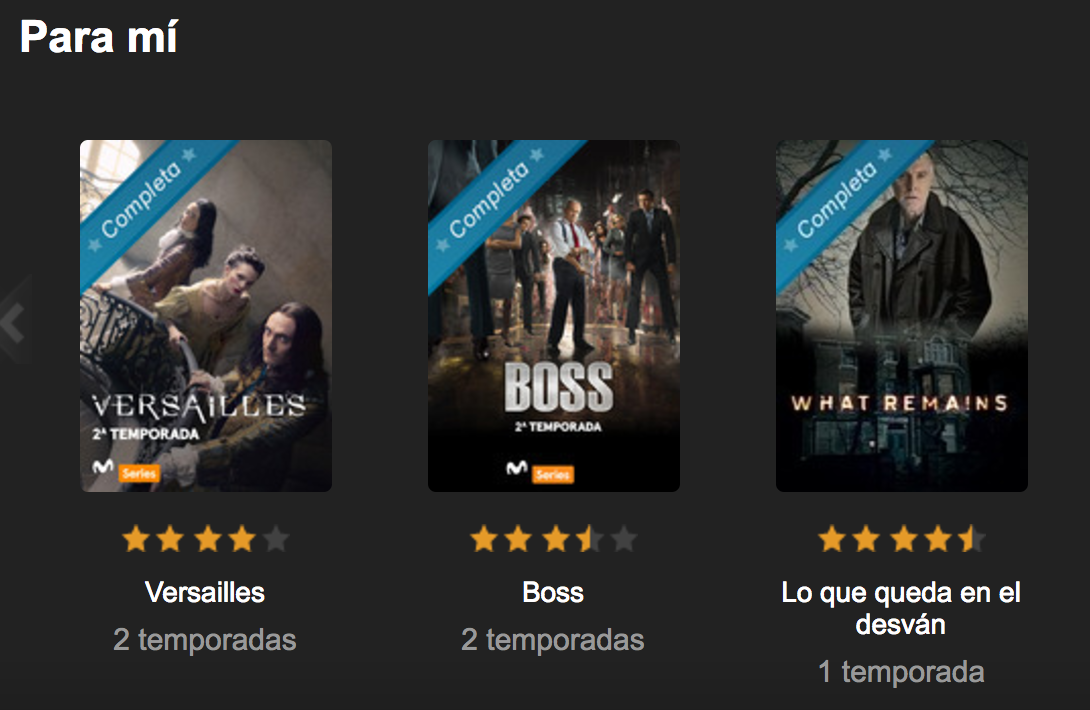
\includegraphics[width=\textwidth]{./figures/rec-movistar.png}
        \caption{Recomendaciones personalizadas en Movistar+\index{Movistar+}}\label{rec-movistar}
    \end{subfigure}
    \begin{subfigure}[t]{0.39\textwidth}
        \centering
        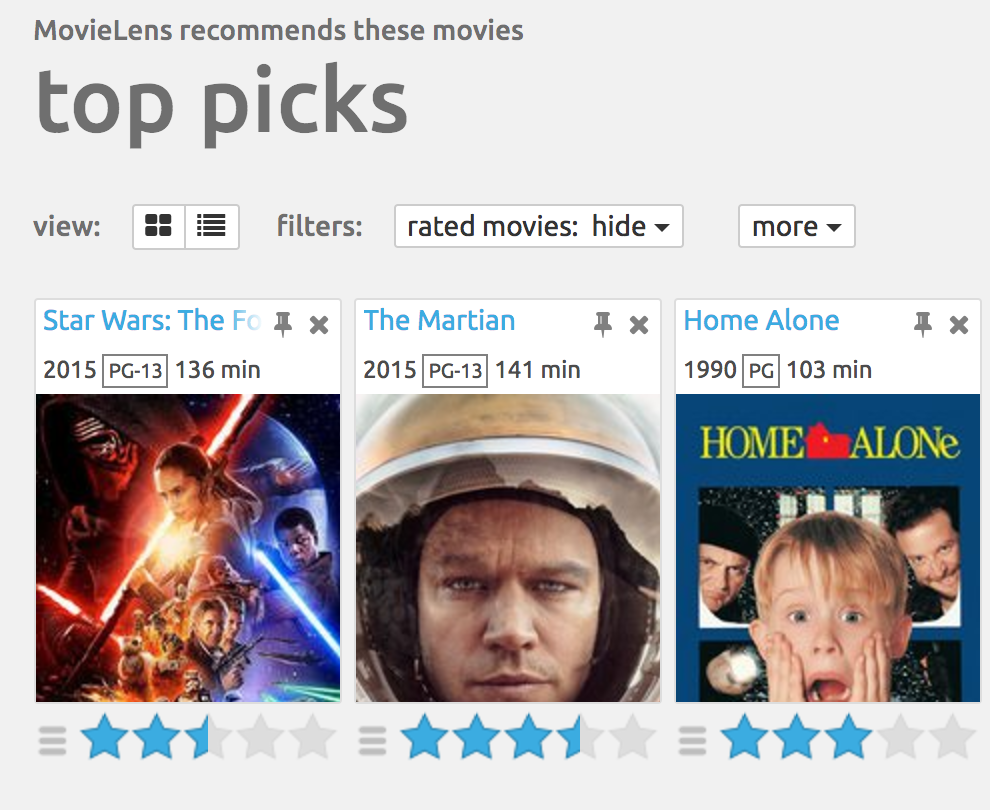
\includegraphics[width=\textwidth]{./figures/rec-movielense.png}
        \caption{Recomendaciones personalizadas en Movielense}\label{rec-movielense}
    \end{subfigure}
    \caption{Sistemas de recomendación basados en filtrado colaborativo}
\end{figure}

\section{Filtrado por contenido}
Este tipo de filtrado relaciona los gustos de un usuario con las propiedades de un ítem sin tener en cuenta a otros usuarios.

Las características de los ítems pueden ser de todo tipo. En las películas podría ser los géneros que le corresponden, en restaurantes el tipo de comida que sirven, etc

Para realizar las recomendaciones los sistemas se suelen basar en acciones anteriores de un usuario para poder recomendar algo (al comprar unos neumáticos recomendar un recambio de aceite, por ejemplo), o se puede crear un modelo en base a los descriptores de los ítems usando redes neuronales, \acrshort{tfidf}\index{TF-IDF}, redes bayesianas, clusters, árboles de decisión etc.

IMDb\index{IMDb} (figura~\ref{rec-imdb}) usa este tipo de sistema para hacer sus recomendaciones al visitar la página de una película.
\begin{figure}[!htbp]
    \centering
    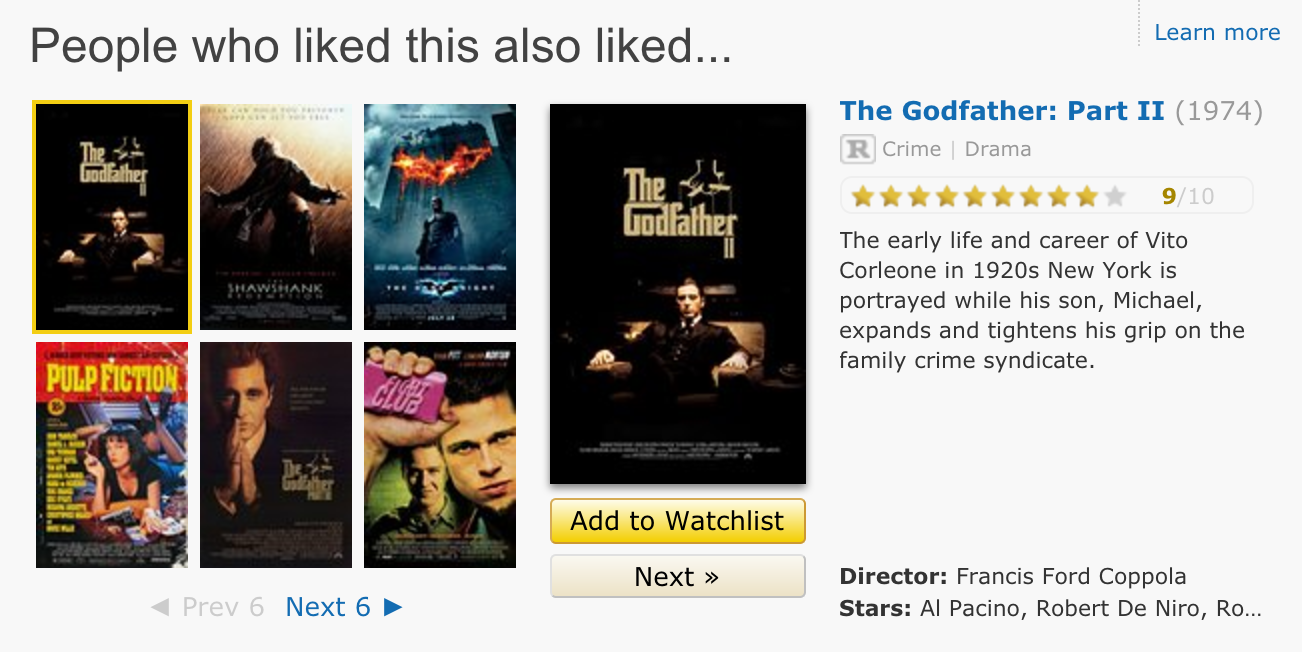
\includegraphics[width=0.8\textwidth]{./figures/rec-imdb.png}
    \caption{Recomendaciones por película en IMDb\index{IMDb}}\label{rec-imdb}
\end{figure}

\section{Evaluación de modelos y otras consideraciones}
La evaluación de estos modelos puede presentar algún problema, ya que no se suele contar un \textit{`\gls{groundtruth}'} contra los que evaluar la precisión del modelo. Por esto se suele evaluar de manera manual y preguntando por la satisfacción de los usuarios o usando \gls{testing-ab}\cite{Beel:2013:CAO:2532508.2532511}.

Además, a la hora de recomendar, los usuarios también suelen valorar otros aspectos que el sistema de recomendación no tome en cuenta.

Por ejemplo, es interesante que las recomendaciones sorprendan\cite{Onuma2009} al usuario y que sean lo suficientemente diferentes entre sí. También es interesante hacer recomendaciones diferentes teniendo en cuenta el lugar donde el usuario vive o su edad. Esto puede suponer problemas ya que el usuario se puede dar cuenta de que el sistema no respeta su privacidad.

\section{Antecedentes}
Existen varias técnicas usadas a día de hoy para recomendar películas. Varios servicios cuentan con recomendaciones por película como \href{http://www.imdb.com}{IMDb}\index{IMDb} (figura~\ref{rec-imdb}) y \href{http://ver.movistarplus.es}{Movistar+}\index{Movistar+}. Otros servicios ofrecen recomendaciones con filtrado colaborativo a cada usuario como \href{https://netflix.com}{Netflix}\index{Netflix} y \href{http://ver.movistarplus.es}{Movistar+}\index{Movistar+} (figura~\ref{rec-movistar}). Además existen servicios que se dedican exclusivamente a hacer estas recomendaciones como \href{https://movielens.org/}{Movielense} (figura~\ref{rec-movielense}), \href{http://www.jinni.com/}{Jinni} y \href{https://www.taste.io/}{Taste.io}.

Muchos de estos servicios se basan en las puntuaciones o visualizaciones de los contenidos vistos por el usuario para realizar un filtrado colaborativo. Otros servicios usan tags, como los ofrecidos por IMDb\index{IMDb} y los géneros, para ver que películas tienen más cosas en común y así poder recomendarlas.

En otros ámbitos se usan sistemas similares. \href{https://www.last.fm/}{Last.fm} hace recomendaciones en base a la música que escuchan sus usuarios. Twitter es capaz de recomendar varias cuentas para seguir a sus usuarios usando una combinación de muchas señales\cite{Gupta:2013:WFS:2488388.2488433}, como se puede ver en la figura~\ref{rec-twitter}.

\begin{figure}[!htbp]
    \centering
    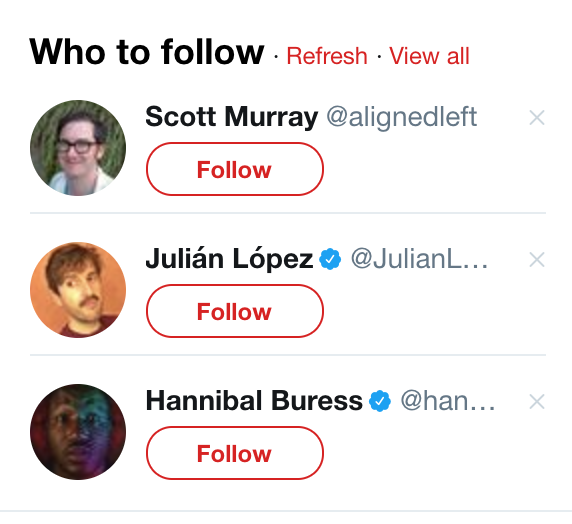
\includegraphics[width=0.4\textwidth]{./figures/rec-twitter.png}
    \caption{Recomendaciones en Twitter}\label{rec-twitter}
\end{figure}

\section{Objetivos}
El objetivo principal es la creación de una aplicación web donde un usuario pueda escoger una película y obtenga 10 películas recomendadas usando diferentes algoritmos basados en el procesamiento de lenguaje natural.

En concreto se implementarán modelos basados en \acrshort{lsa}\index{LSA} y Doc2Vec\index{Doc2Vec}, además de realizar una optimización de sus parámetros para su evaluación. También se describirá un tercer modelo híbrido llamado E-Modelo\cite{emodelo}\index{E-Modelo}, que, pese a haber completado su implementación, no se ha incluido en el recomendador.

También se implementa una interfaz común donde poder hacer peticiones a los diferentes modelos usando una \acrshort{api} \acrshort{rest}, además de la interfaz web desde donde probar los algoritmos. Ésta última debe ser rápida y lo suficientemente intuitiva para que un usuario normal lo pueda usar. La \acrshort{api} \acrshort{rest} es pública y puede servir para la creación de otros servicios ajenos a este proyecto.

Para la creación de modelos es necesario tener un buen conjunto de datos con los que realizar el entrenamiento. Para ello se realiza otro programa que descarga los datos necesarios de IMDb\index{IMDb} mediante un crawler.

El código del proyecto está publicado en tres repositorios de GitHub (todo el código bajo licencia MIT):

\begin{itemize}
    \item \textit{Frontend} \url{https://github.com/hugo19941994/movie-pepper-back}
    \item \textit{Backend} \url{https://github.com/hugo19941994/movie-pepper-front}
    \item \textit{Documentación} \url{https://github.com/hugo19941994/movie-pepper-doc}
\end{itemize}

El proyecto está en producción y se puede visitar en \url{https://moviepepper.hugofs.com}.

\section{Estructura}
En primer lugar se describe la metodología seguida para el desarrollo del proyecto, mientras que los capítulos siguientes se centran en la parte mas técnica del proyecto y describen los diferentes procesos y métodos usados. Esto incluye como se consiguen los datos para el recomendador, como se filtra el texto y los algoritmos usados para la creación de los modelos.

En segundo lugar se presentan unas gráficas con los resultados al variar los parámetros de los dos algoritmos implementados y unos resultados finales con los modelos finalizados.

El capítulo \textit{Interfaz} habla sobre la web desde donde se pueden probar los modelos y como se ha creado.

Finalmente se presentan unas conclusiones sobre el proyecto y se habla sobre partes que se podrían mejorar.

\chapter{Metodología}
La metodología de este proyecto ha sido ágil, basado en la creación de \acrshort{mvp}s. Gracias a esta metodología se pueden evaluar diferentes caminos e hipótesis posibles con una cantidad de recursos limitados. También reduce los riesgos frente a posibles fallos o experimentos.

Cada iteración del proyecto constaba con unos objetivos claros y un alcance limitado. Después de su realización se lanzaban una serie de pruebas para verificar su correcto funcionamiento y se analizaban los resultados obtenidos. Si los resultados no fueron satisfactorios se descartaba esta iteración y se realizaba alguna modificación para poder ir mejorando.

En primer lugar realizamos la fase de recolección de datos. Se probaron tres sitios diferentes: Wikipedia\index{Wikipedia}, IMDb\cite{imdb}\index{IMDb} y FilmAffinity\index{FilmAffinity}. En Wikipedia\index{Wikipedia} es demasiado difícil sacar la información de las diferentes películas manera precisa. Tanto FilmAffinity como IMDb\cite{imdb}\index{IMDb} tienen contenidos más estructurados. FilmAffinity\index{FilmAffinity} tiene tags de género más precisos, pero IMDb\cite{imdb}\index{IMDb} cuenta con muchos más usuarios y por lo tanto más variedad de tags y de críticas.

Se empezó usando una combinación de las 3 fuentes, pero tras hacer pruebas se vio que con los datos de IMDb\cite{imdb}\index{IMDb} era suficiente y simplificaba el código.

También se usó \Gls{mongodb} para guardar toda la información, pero finalmente se descartó por el mismo motivo de arriba. Complicaba el código y en este proyecto no aportaba muchos beneficios, sobre todo al eliminar la información de FilmAffinity\index{FilmAffinity} y Wikipedia\index{Wikipedia}.

Como orden de implementación se realizó primero el modelo \acrshort{lsa}\index{LSA} y en paralelo se realizó el proyecto de E-Modelo\cite{emodelo}\index{E-Modelo}. Debido a las resultados del E-Modelo\index{E-Modelo} se decidió reemplazarlo con Doc2Vec\index{Doc2Vec}.

Cuando todos los modelos fueron optimizados y evaluados se realizó la interfaz web, el \acrshort{api} \acrshort{rest} y este documento.

Hay que mencionar que la inspiración para este proyecto fue la realización de tareas de mejora e investigación en un motor de recomendación de películas al hacer el practicum, aunque el código en sí no guarda ninguna relación.

\begin{figure}[!htbp]
    \centering
    \begin{ganttchart}[
        hgrid,
        vgrid,
        time slot format=isodate-yearmonth,
        compress calendar
        ]{2016-9}{2017-7} %chktex 8
        \setganttlinklabel{f-s}{}

        \gantttitlecalendar{year, month} \\
        \ganttbar{Investigación}{2016-09}{2016-11} \\ %chktex 8
        \ganttbar{Doc2Vec}{2017-03}{2017-03} \\ %chktex 8
        \ganttbar{LSA MVP1}{2016-10}{2016-11} \\ %chktex 8
        \ganttbar{LSA MVP2}{2016-12}{2017-01} \\ %chktex 8
        \ganttbar{LSA MVP3}{2017-02}{2017-03} \\ %chktex 8
        \ganttbar{ALS MVP1}{2016-09}{2016-12} \\ %chktex 8
        \ganttbar{ALS MVP2}{2017-01}{2017-02} \\ %chktex 8
        \ganttbar{ALS MVP3}{2017-03}{2017-03} \\ %chktex 8
        \ganttbar{Desarrollo Interfaz}{2017-04}{2017-05} \\ %chktex 8
        \ganttmilestone{Fin Desarrollo}{2017-05} \\ %chktex 8
        \ganttbar{Documentación}{2017-05}{2017-06} \\ %chktex 8
        \ganttmilestone{Entrega \& Presentación}{2017-06}{2017-06} %chktex 8

        \ganttlink{elem0}{elem1}
        \ganttlink{elem0}{elem2}

        \ganttlink[link type=f-s]{elem2}{elem3}
        \ganttlink[link type=f-s]{elem3}{elem4}

        \ganttlink[link type=f-s]{elem5}{elem6}
        \ganttlink[link type=f-s]{elem6}{elem7}

        \ganttlink[link type=f-s]{elem1}{elem8}
        \ganttlink[link type=f-s]{elem4}{elem8}
        \ganttlink[link type=f-s]{elem7}{elem8}

        \ganttlink{elem8}{elem9}
        \ganttlink{elem10}{elem11}
    \end{ganttchart}
    \caption{Diagrama de Gantt con tiempos del proyecto}
\end{figure}


\chapter{Recolección de datos}
El primer paso es la obtención de datos con los que hacer las recomendaciones y entrenar los modelos. Para esta tarea se ha usado Scrapy\cite{scrapy}, un paquete de Python\index{Python} con el que crear crawlers de Internet.

\begin{figure}[!htbp]
    \begin{tikzpicture}[node distance=2cm]
        \centering
        \node (init) [startstop] {Top 1000 IMDb};
        \node (link1) [decision, below of=init] {URL};
        \node (pelicula-init) [startstop, below of=link1] {Película};
        \node (link2) [decision, below of=pelicula-init, yshift=-2cm] {URL};
        \node (keywords) [process, right of=link2, xshift=2cm] {Palabras clave};
        \node (info) [process, above of=keywords] {Información};
        \node (reviews) [startstop, below of=link2] {Críticas};
        \node (link3) [decision, below of=reviews] {URL};
        \node (reviews-1) [process, right of=reviews, xshift=2cm] {Crítica};
        \node (database) [database, right of=link1, xshift=3cm] {BD};
        \begin{scope}[on background layer]
            \node (bbox) [rectangle,draw,minimum width=2cm] [fit = (info) (keywords) (reviews-1),fill=yellow!30,label=above:Película] {};
        \end{scope}

        \draw [line] (init) -- (link1);
        \draw [line] (link1) to [bend left] node[anchor=east] {página} (init);
        \draw [line] (link1) -- node[anchor=north] {¿visitado?} (database);
        \draw [line] (database) |- node[anchor=west] {no} (pelicula-init);
        \draw [line] (pelicula-init) -- (link2);
        \draw [line] (pelicula-init) |- (info);
        \draw [line] (link2) -- (keywords);
        \draw [line] (link2) -- (reviews);
        \draw [line] (reviews) -- (link3);
        \draw [line] (link3) to [bend left] node[anchor=east] {página} (reviews);
        \draw [line] (link3) -| (reviews-1);
    \end{tikzpicture}
    \caption{Diagrama de flujo de la descarga de datos}
\end{figure}

El crawler inicia a indexar en la pagina de top 1000 películas por valoración de los usuarios (link). El crawler descarga los siguientes datos de cada película.

\setlength{\columnseprule}{0pt}
\begin{multicols}{2}
    \begin{itemize}
        \item Título
        \item Directores
        \item Año
        \item Género
        \item Sinopsis
        \item Críticas
        \item Palabras claves
        \item Carátula
        \item URL
    \end{itemize}
\end{multicols}

El crawler entra en todos los enlaces de la pagina inicial. Si el siguiente enlace es la siguiente lista de películas repite el proceso. Si el enlace pertenece a una película se descarga los datos y busca la pagina de las keywords, sinopsis y criticas. Si el enlace no es la ficha de una película ni parte de la lista se descarta. Este proceso termina cuando no queda ningún enlace por indexar. Este proceso se realiza de manera asíncrona (explicar) usando Python\index{Python} 3.6.

Como criticas se descargan como máximo las 25 con mejores valoraciones. Esto, junto a la sinopsis forman los datos con los que entrenar tanto el modelo Doc2Vec\index{Doc2Vec} como el \acrshort{lsa}\index{LSA}.

Todo el texto descargado esta en inglés. Si algunos de los datos estuviese en otro idioma sería necesario traducirlo o descartarlo. En una primera versión se descargaban datos tanto en inglés como en español y se traducía usando la \href{https://www.microsoft.com/en-us/translator/translatorapi.aspx}{acrshort{api} de traducción de Microsoft}. Finalmente se eliminó, ya que por lo general la mayoría de contenido del top 1000 de IMDb\cite{imdb}\index{IMDb} es de habla inglesa, al igual que la mayoría de críticas escritas allí. Eliminando los datos en castellano se simplificaba el código y se elimina una dependencia de un servicio externo.

Toda la información se guarda en ficheros \acrshort{json}\index{JSON}. Un ejemplo de documento es:

\inputminted[xleftmargin=21pt, breaklines=true, tabsize=2]{json}{figures/example.json}

\chapter{Limpieza de textos}\label{chap:clean}
El preprocesado de los textos es una parte esencial del procesamiento del lenguaje natural. Sin este paso la precisión del modelo es mucho menor ya que el modelo tendrá mucho ruido. Es importante eliminar todas las ambigüedades posibles para poder relacionar los conceptos que existen dentro de los textos y así ayudar a los algoritmos a cumplir su función.

Algunas de las técnicas más comunes incluyen eliminar tiempos verbales, signos de puntuación, distinción entre palabras singulares y plurales, masculinas y femeninas, mayúsculas y minúsculas, palabras muy comunes, etc.\

\section{POS Tagger}
En primer lugar separamos cada documento en frases. Se usa un POS Tagger entrenado con el Penn Treebank tagset\cite{penn-treebank} (el tagger por defecto de NLTK\cite{NLTK}):

\begin{verbatim}
    Zeus is a Greek God.
\end{verbatim}

Quedaría tagueado así

\begin{figure}[!htbp]
    \centering
    \inline{Zeus}{NNP} \inline{is}{VBZ} \inline{a}{DT} \inline{Greek}{NN} \inline{God}{NNP}.
    \floatfoot{Donde NNP es nombre propio, VBZ un verbo, DT determinante y NN nombre común}
    \caption{Resultados del POS tagging}
\end{figure}

\section{Reemplazar sustantivos por hiperónimos}
Cualquier sustantivo se intenta reemplazar por un hiperónimo (palabra de la misma familia pero de categoría más general, como animal es a perro o audio a altavoz). Para obtener el hiperónimo de forma precisa usamos la función lesk\cite{Lesk:1986:ASD:318723.318728} de NLTK\cite{NLTK}, que detecta el contexto de una palabra (es capaz de diferenciar gato de herramienta a gato de animal dependiendo de las palabras que rodean a la palabra en cuestión).

El resultado de lesk\cite{Lesk:1986:ASD:318723.318728} es una lista ordenada por relevancia de hiperónimos del blob. Se reemplaza por el primer resultado (el más relevante).

Así el texto se convertirá en:
\begin{center}
    \begin{verbatim}
        Zeus is a country deity.
    \end{verbatim}
\end{center}

\section{Eliminación de nombres propios}
Los nombres propios se eliminan porque se detectó que si dos personajes de películas diferentes se llamaban igual la similitud resultante de los cálculos con \acrshort{lsa}\index{LSA} muy alta, aunque las películas no tengan nada que ver. Para evitar esto se eliminan.

Así el texto se convertirá en:
\begin{verbatim}
    is a country deity.
\end{verbatim}

\section{Filtrar Stopwords}
En este paso se elimina cualquier token que coincida con los stopwords de la lista inglesa de NLTK\cite{NLTK} y cualquier número. Esta lista incluye palabras muy comunes como `i', `me', `my', `am', `those', `few', etc.

También se eliminan los signos de puntuación y se pasan todas las palabras a minúsculas.

Nuestro texto anterior ahora se convertirá en:
\begin{verbatim}
    country deity
\end{verbatim}

\section{Stemmer}
El ultimo paso del filtrado del texto es pasar el SnowBall\cite{snowball} stemmer de NLTK\cite{NLTK}\@. En este caso Snowball usa el algoritmo de Porter\cite{porter}.

El stemming reduce cualquier palabra a su raíz, eliminando las partes de palabras que las hacen plurales, masculino o femenino y  diferentes tiempos verbales, entre otros. Esto permite a nuestro recomendador interpretar palabras similares en los diferentes documentos como iguales. Algunos ejemplos:

\begin{center}
consign $\Rightarrow$ consign

consigned $\Rightarrow$ consign

consigning $\Rightarrow$ consign

consignment $\Rightarrow$ consign
\end{center}

Siguiendo con el mismo ejemplo:
\begin{verbatim}
    counti deiti
\end{verbatim}

Esto relacionará palabras como counties, country, countries, etc.

\chapter{LSA}\label{chap:lsa}
\acrfull{lsa} es el algoritmo en el que se basa el primer modelo de recomendación implementado en el proyecto. Se trata de una serie de técnicas usadas para determinar la distribución semántica y la relación entre documentos extrayendo conceptos. La hipótesis principal de \acrshort{lsa} es que las palabras que tienen alguna relación relación semántica ocurrirán en documentos que también tienen una relación.

Estas técnicas se empezaron a desarrollar en los años 60\cite{Borko:1963:ADC:321160.321165}, pero se popularizaron en los años 90\cite{Deerwester90indexingby}. A día de hoy sigue siendo una de las técnicas más usadas dentro del procesamiento del lenguaje natural.

\section{TF-IDF}
El \acrfull{tfidf}\index{TF-IDF} calcula lo relevante que es una palabra dentro de un conjunto de documentos.Construye una matriz de relevancia por documento, donde cada casilla representa la relevancia de un termino en él. Cuanto más aparece un termino en un documento, más relevante es, pero cuanto más aparece en global, menos peso tendrá. El 83\% de los recomendadores que usan textos se basan en este algoritmo\cite{Beel2016}.

Algunos de los parámetros que se pueden ajustar son el número mínimo y máximo de veces que un termino puede aparecer en el conjunto para entrar dentro del calculo. También se puede ajustar el número de palabras máximas a analizar. Si ese número se sobrepasa se eliminan las palabras con menos relevancia. En el \autoref{chap:opt} se ajustarán los parámetros para ver cuales son los idóneos para esta tarea.

\begin{equation} \label{eq:tf-idf}
    tfidf(t, d, D) = tf(t, d) \cdot idf(t, D)
\end{equation}

\begin{equation} \label{eq:tf}
    tf(t, d) = \dfrac{f_{t, d}}{\sum_{t' \epsilon d}^{}f_{t', d}}
\end{equation}

\begin{equation} \label{eq:idf}
    idf(t, d) = \log\biggl(\dfrac{|D|}{1 + \{d \epsilon D : t \epsilon d \}}\biggr)
\end{equation}

Para cada conjunto de documentos filtrados se hace el \acrshort{tfidf}\index{TF-IDF} y quedan las palabras mas relevantes de cada película. Un pequeño ejemplo sería:

\begin{figure}[!htbp]
    \centering
    \[tfidf =
        \begin{tikzpicture}[baseline=-0.65ex,scale=0.8]
            \matrix [matrix of math nodes,left delimiter=(,right delimiter=),row sep=0.5cm,column sep=0.5cm] (m) {
                0.39&0.16&0.19&0.01&0.25&0.79&0.27 \\
                0.12&0.12&0.06&0.46&0.21&0.07&0.83 \\
                0.46&0.55&0.15&0.55&0.22&0.27&0.11 \\
                0.00&0.60&0.51&0.00&0.00&0.60&0.00 \\
                0.41&0.00&0.35&0.83&0.00&0.00&0.00 \\
            };
            \node[above=10pt of m-1-1, rotate=45, yshift=3mm, xshift=3mm] (top-1) {says};
            \node[above=10pt of m-1-2, rotate=45, yshift=3mm, xshift=3mm] (top-2) {just};
            \node[above=10pt of m-1-3, rotate=45, yshift=3mm, xshift=3mm] (top-3) {room};
            \node[above=10pt of m-1-4, rotate=45, yshift=3mm, xshift=3mm] (top-4) {dead};
            \node[above=10pt of m-1-5, rotate=45, yshift=3mm, xshift=3mm] (top-5) {asks};
            \node[above=10pt of m-1-6, rotate=45, yshift=3mm, xshift=3mm] (top-6) {ship};
            \node[above=10pt of m-1-7, rotate=45, yshift=3mm, xshift=3mm] (top-7) {mother};

            \node[left=12pt of m-1-1] (left-1) {The Matrix};
            \node[left=12pt of m-2-1] (left-2) {Alien};
            \node[left=12pt of m-3-1] (left-3) {Serenity};
            \node[left=12pt of m-4-1] (left-4) {Casablanca};
            \node[left=12pt of m-5-1] (left-5) {Amelie};
        \end{tikzpicture}
    \]
    \caption{Ejemplo matriz \acrshort{tfidf}\index{TF-IDF}}
\end{figure}

Esto crea una matriz donde cada fila corresponde a un documento del corpus, mientras que las columnas representan las palabras del vocabulario. Cada casilla corresponde a la relavancia de esa palabra en ese documento. En nuestro caso guardamos cada fila en el \acrshort{json} de la películas correspondiente. Si fuese necesario, en este paso se pueden extraer los tokens más relevantes de cada documento para su posterior uso. Cuando se ejecute \acrshort{svd}\index{SVD} se perderán esos datos, pero para el recomendador no va a ser necesario guardarlos.

El código para realizar la matriz \acrshort{tfidf} se basa en la implementación de scikit-learn\cite{scikit-learn}

\section{Descomposición en valores singulares}
Con \acrfull{svd}\index{SVD} reducimos la dimensionalidad de la matriz calculada con \acrshort{tfidf}\index{TF-IDF}. Esto acelera de una manera muy significativa los cálculos y además soluciona el problema de la polisemia. Existen varias formas de calcular el \acrshort{svd}\index{SVD}, pero scikit-learn implementa el algoritmo descrito en \citetitle{2009arXiv0909.4061H}

\acrshort{svd}\index{SVD} busca descomponer una matriz natural en 3 matrices diferentes diferentes. A representa la matriz de documentos donde cada fila representa los diferentes términos y las columnas representan los diferentes documentos.\cite{stanford-svd}

\begin{figure}[!htbp]
    \centering
    \[A =
        \begin{tikzpicture}[baseline=-0.65ex,scale=0.8]
            \matrix [matrix of math nodes,left delimiter=(,right delimiter=),row sep=0.5cm,column sep=0.5cm] (m) {
                1&1&1&0&0 \\
                3&3&3&0&0 \\
                4&4&4&0&0 \\
                5&5&5&0&0 \\
                0&2&0&4&4 \\
                0&0&0&5&5 \\
                0&1&0&2&2 \\
            };
            \node[above=10pt of m-1-1, rotate=45, yshift=3mm, xshift=3mm] (top-1) {Matrix};
            \node[above=10pt of m-1-2, rotate=45, yshift=3mm, xshift=3mm] (top-2) {Alien};
            \node[above=10pt of m-1-3, rotate=45, yshift=3mm, xshift=3mm] (top-3) {Serenity};
            \node[above=10pt of m-1-4, rotate=45, yshift=3mm, xshift=3mm] (top-4) {Casablanca};
            \node[above=10pt of m-1-5, rotate=45, yshift=3mm, xshift=3mm] (top-5) {Amelie};

            \node[left=12pt of m-1-1] (left-1) {action};
            \node[left=12pt of m-2-1] (left-2) {gun};
            \node[left=12pt of m-3-1] (left-3) {shoot};
            \node[left=12pt of m-4-1] (left-4) {run};
            \node[left=12pt of m-5-1] (left-5) {love};
            \node[left=12pt of m-6-1] (left-6) {peace};
            \node[left=12pt of m-7-1] (left-7) {kiss};

            \node[rectangle,left delimiter=\{, xshift=-3mm] (del-left-1) at ($0.6*(left-1.east) + 0.5*(left-4.east)$) {\tikz{\path (left-1.north east) rectangle (left-4.south west);}};
            \node[left=10pt] at (del-left-1.west) {Action};
            \node[rectangle,left delimiter=\{, xshift=-3mm] (del-left-2) at ($0.6*(left-5.east) + 0.5*(left-7.east)$) {\tikz{\path (left-5.north east) rectangle (left-7.south west);}};
            \node[left=10pt] at (del-left-2.west) {Romantic};

        \end{tikzpicture}
        = U \cdot \Sigma \cdot V^T
    \]
    \caption{Ejemplo matriz \acrshort{lsa}\index{LSA}}
\end{figure}

\begin{figure}[!htbp]
    \centering
    \[
        U =
        \begin{tikzpicture}[baseline=-0.65ex,scale=0.8]
            \matrix [matrix of math nodes,left delimiter=(,right delimiter=),row sep=0.5cm,column sep=0.5cm] (m) {
                0.13&0.02&-0.01& \\
                0.41&0.07&-0.03& \\
                0.55&0.09&-0.04& \\
                0.68&0.11&-0.05& \\
                0.15&-0.59&0.65& \\
                0.07&-0.73&0.67& \\
                0.07&-0.29&0.32& \\
            };

            \node[above=10pt of m-1-1, rotate=45, yshift=3mm, xshift=5mm] (top-1) {Sci-Fi topic};
            \node[above=10pt of m-1-2, rotate=45, yshift=3mm, xshift=5mm] (top-2) {Romance topic};
            \node[above=10pt of m-1-3, rotate=45, yshift=3mm, xshift=5mm] (top-3) {Ruido};

            \node[left=12pt of m-1-1] (left-1) {action};
            \node[left=12pt of m-2-1] (left-2) {gun};
            \node[left=12pt of m-3-1] (left-3) {shoot};
            \node[left=12pt of m-4-1] (left-4) {run};
            \node[left=12pt of m-5-1] (left-5) {love};
            \node[left=12pt of m-6-1] (left-6) {peace};
            \node[left=12pt of m-7-1] (left-7) {kiss};

        \end{tikzpicture}
    \]
    \floatfoot{Donde U se considera la matriz palabra-a-categoría}
    \caption{Matriz \acrshort{lsa}\index{LSA} palabra a categoría}
\end{figure}

\begin{figure}[!htbp]
    \centering
    \[
        \Sigma =
        \begin{tikzpicture}[baseline=-0.65ex,scale=0.8]
            \matrix [matrix of math nodes,left delimiter=(,right delimiter=),row sep=0.5cm,column sep=0.5cm] (m) {
                12.4&0&0& \\
                0&9.5&0& \\
                0&0&1.3& \\
            };

            \node[above=10pt of m-1-1, rotate=45, yshift=3mm, xshift=5mm] (top-1) {Sci-Fi topic};
            \node[above=10pt of m-1-2, rotate=45, yshift=3mm, xshift=5mm] (top-2) {Romance topic};
            \node[above=10pt of m-1-3, rotate=45, yshift=3mm, xshift=5mm] (top-3) {Ruido};
        \end{tikzpicture}
    \]
    \floatfoot{Donde $\Sigma$ se considera la matriz de importancia de cada categoría}
    \caption{Ejemplo matriz $\Sigma$ de \acrshort{lsa}\index{LSA}}\label{matrix-topics}
\end{figure}

\begin{figure}[!htbp]
    \centering
    \[
        V^T =
        \begin{tikzpicture}[baseline=-0.65ex,scale=0.8]
            \matrix [matrix of math nodes,left delimiter=(,right delimiter=),row sep=0.5cm,column sep=0.5cm] (m) {
                0.56&0.59&0.56&0.09&0.09 \\
                0.12&-0.02&0.12&-0.69&-0.69 \\
                0.40&-0.80&0.40&0.09&0.09 \\};

            \node[above=10pt of m-1-1, rotate=45, yshift=3mm, xshift=3mm] (top-1) {Matrix};
            \node[above=10pt of m-1-2, rotate=45, yshift=3mm, xshift=3mm] (top-2) {Alien};
            \node[above=10pt of m-1-3, rotate=45, yshift=3mm, xshift=3mm] (top-3) {Serenity};
            \node[above=10pt of m-1-4, rotate=45, yshift=3mm, xshift=3mm] (top-4) {Casablanca};
            \node[above=10pt of m-1-5, rotate=45, yshift=3mm, xshift=3mm] (top-5) {Amelie};

            \node[left=12pt of m-1-1] (left-1) {Sci-Fi topic};
            \node[left=12pt of m-2-1] (left-2) {Romance topic};
            \node[left=12pt of m-3-1] (left-3) {Ruido};

        \end{tikzpicture}
    \]
    \floatfoot{$V^T$ se considera la matriz de documento-a-categoría}
    \caption{Matriz \acrshort{lsa}\index{LSA} documento a categoría}\label{matrix-dac}
\end{figure}

Es importante recordar que para cualquier matriz natural A es posible calcular su \acrshort{svd}\index{SVD} donde:
U, $\Sigma$ \& V son únicos
U \& V son ortonormales:
\begin{equation}
    U^T \cdot U = I
\end{equation}

\begin{equation}
    V^T \cdot V = I
\end{equation}
$\Sigma$ es diagonal y sus valores singulares están en orden descendiente ($\sigma_{1}$ > $\sigma_{2}$ > $\sigma_{3}$\ldots)

Estas matrices se guardan en el mismo documento dentro de la base de datos y se usan a la hora de recomendar haciendo la distancia del coseno entre las matrices de dos películas. La implementación del \acrshort{lsa}\index{LSA} también se basa en la de scikit-learn\cite{scikit-learn}

También es normal reducir la dimensionalidad eliminando los conceptos que tengan menor relevancia en nuestros cálculos. En este ejemplo, el concepto llamado `Ruido' tiene una relevancia mucho menor que los otros dos conceptos (figura~\ref{matrix-topics}), y por tanto se puede eliminar ya que no aportará mucha información (figura~\ref{reduced-matrix-dac}).

\begin{figure}[!htbp]
    \centering
    \[
        V^T =
        \begin{tikzpicture}[baseline=-0.65ex,scale=0.8]
            \matrix [matrix of math nodes,left delimiter=(,right delimiter=),row sep=0.5cm,column sep=0.5cm] (m) {
                0.56&0.59&0.56&0.09&0.09 \\
                0.12&-0.02&0.12&-0.69&-0.69 \\};

            \node[above=10pt of m-1-1, rotate=45, yshift=3mm, xshift=3mm] (top-1) {Matrix};
            \node[above=10pt of m-1-2, rotate=45, yshift=3mm, xshift=3mm] (top-2) {Alien};
            \node[above=10pt of m-1-3, rotate=45, yshift=3mm, xshift=3mm] (top-3) {Serenity};
            \node[above=10pt of m-1-4, rotate=45, yshift=3mm, xshift=3mm] (top-4) {Casablanca};
            \node[above=10pt of m-1-5, rotate=45, yshift=3mm, xshift=3mm] (top-5) {Amelie};

            \node[left=12pt of m-1-1] (left-1) {Sci-Fi topic};
            \node[left=12pt of m-2-1] (left-2) {Romance topic};

        \end{tikzpicture}
    \]
    \floatfoot{$V^T$ después de la eliminación del concepto `Ruido'}
    \caption{Matriz \acrshort{lsa}\index{LSA} documento a categoría reducida}\label{reduced-matrix-dac}
\end{figure}

\section{Similitud del coseno}
Para obtener los valores finales de \acrshort{lsa}\index{LSA} se debe calcular la similitud del coseno entre los vectores de documentos. Esto nos da un valor entre -1 y 1 pero como nos movemos en un espacio positivo los valores finales serán entre 0 y 1. En las figuras~\ref{cos-low} y~\ref{cos-high} se puede ver una representación gráfica en 2D.

\begin{equation}
    \cos(\theta) = \dfrac{\sum_{i=1}^{n} A_i \cdot B_i}{\sqrt{\sum_{i=1}^{n} A_i^2} \cdot \sqrt{\sum_{i=1}^{n} B_i^2}}
\end{equation}

Siguiendo con el ejemplo anterior:

\begin{figure}[!htbp]
    \begin{equation}
        \cos\left(
            \begin{tikzpicture}[baseline=-0.65ex,scale=0.8]
                \matrix [matrix of math nodes,left delimiter=(,right delimiter=),row sep=0.5cm,column sep=0.5cm] (m) {0.56\\0.12\\};
            \end{tikzpicture}
            ,
            \begin{tikzpicture}[baseline=-0.65ex,scale=0.8]
                \matrix [matrix of math nodes,left delimiter=(,right delimiter=),row sep=0.5cm,column sep=0.5cm] (m) {0.59\\-0.02\\};
            \end{tikzpicture}
        \right) = 0.97
    \end{equation}
    \caption{Alta similitud entre Matrix y Alien}
\end{figure}

\begin{figure}[!htbp]
    \begin{equation}
        \cos\left(
            \begin{tikzpicture}[baseline=-0.65ex,scale=0.8]
                \matrix [matrix of math nodes,left delimiter=(,right delimiter=),row sep=0.5cm,column sep=0.5cm] (m) {0.56\\0.12\\};
            \end{tikzpicture}
            ,
            \begin{tikzpicture}[baseline=-0.65ex,scale=0.8]
                \matrix [matrix of math nodes,left delimiter=(,right delimiter=),row sep=0.5cm,column sep=0.5cm] (m) {0.09\\-0.69\\};
            \end{tikzpicture}
        \right) = -0.08
    \end{equation}
    \caption{Baja similitud entre Matrix y Amelie}
\end{figure}

\begin{figure}[!htbp]
    \centering
    \begin{subfigure}[t]{0.4\textwidth}
        \begin{tikzpicture}
            \draw[help lines, color=gray!30, dashed] (-1,-1) grid (4,4);
            \draw[dashed] (0,0)--(4,0);
            \draw[dashed] (0,0)--(0,4);
            \draw[dashed] (0,0)--(-1,0);
            \draw[dashed] (0,0)--(0,-1);
            \draw[arrow] (0,0) -- ++(30:3cm);
            \draw[arrow] (0,0) -- ++(40:3cm);
            \draw ([shift=(30:1cm)]0,0) arc (30:40:1cm) node [above=50pt, xshift=40pt, align=left] {$\theta$=$\sim$10\textdegree\\cos($\theta$)=$\sim$0.98};
        \end{tikzpicture}
        \caption{Alta similitud del coseno}\label{cos-high}
    \end{subfigure}
    \begin{subfigure}[t]{0.4\textwidth}
        \centering
        \begin{tikzpicture}
            \draw[help lines, color=gray!30, dashed] (-1,-1) grid (4,4);
            \draw[dashed] (0,0)--(4,0);
            \draw[dashed] (0,0)--(0,4);
            \draw[dashed] (0,0)--(-1,0);
            \draw[dashed] (0,0)--(0,-1);
            \draw[arrow] (0,0) -- ++(10:3cm);
            \draw[arrow] (0,0) -- ++(80:3cm);
            \draw ([shift=(10:1cm)]0,0) arc (10:80:1cm) node [above, xshift=50pt, align=left] {$\theta$=$\sim$80\textdegree\\cos($\theta$)=$\sim$0.17};
        \end{tikzpicture}
        \caption{Baja similitud del coseno}\label{cos-low}
    \end{subfigure}
    \caption{Visualización de la similitud del coseno}
\end{figure}

\chapter{Doc2Vec}\index{Word2Vec}\index{Doc2Vec}
Word2Vec\cite{DBLP:journals/corr/abs-1301-3781}\index{Word2Vec} es un algoritmo de tipo \Gls{word-embedding} creado por Google en 2013. Doc2Vec\index{Doc2Vec} es es un algoritmo que se basa en Word2Vec\index{Word2Vec} pero trabajando sobre múltiples documentos para así tener vectores de párrafo en vez de vectores de palabras. Fue desarrollado en 2014 por los mismos investigadores de Google\cite{DBLP:journals/corr/LeM14}, aunque no lo llamaron Doc2Vec\index{Doc2Vec} (así se llama la implementación en Gensim\cite{rehurek_lrec}).

Este algoritmo se va a usar para tratar de descubrir que películas tienen más relación entre sí y así poder crear otro modelo de recomendación similar al creado en el \autoref{chap:lsa}.

Para explicar el funcionamiento de Doc2Vec\index{Doc2Vec} es esencial hablar antes de Word2Vec\index{Word2Vec}.

\section{Word2Vec}\index{Word2Vec}
Word2Vec\index{Word2Vec} crea una red neuronal con una única capa oculta. Existen dos modelos, \acrfull{cbow} y Skip-Gram, el segundo dando, por lo general, mejores resultados.

El objetivo del modelo \acrshort{cbow} es predecir la posibilidad de que una palabra aparezca en un contexto dado. Por el contrario, el objetivo de un modelo Skip-Gram es el de predecir que palabras aparecen en el contexto de una palabra. A continuación se explica el funcionamiento, a alto nivel, del modelo Skip-Gram.

\begin{figure}
    \centering
    \begin{subfigure}[t]{0.4\textwidth}
        \centering
        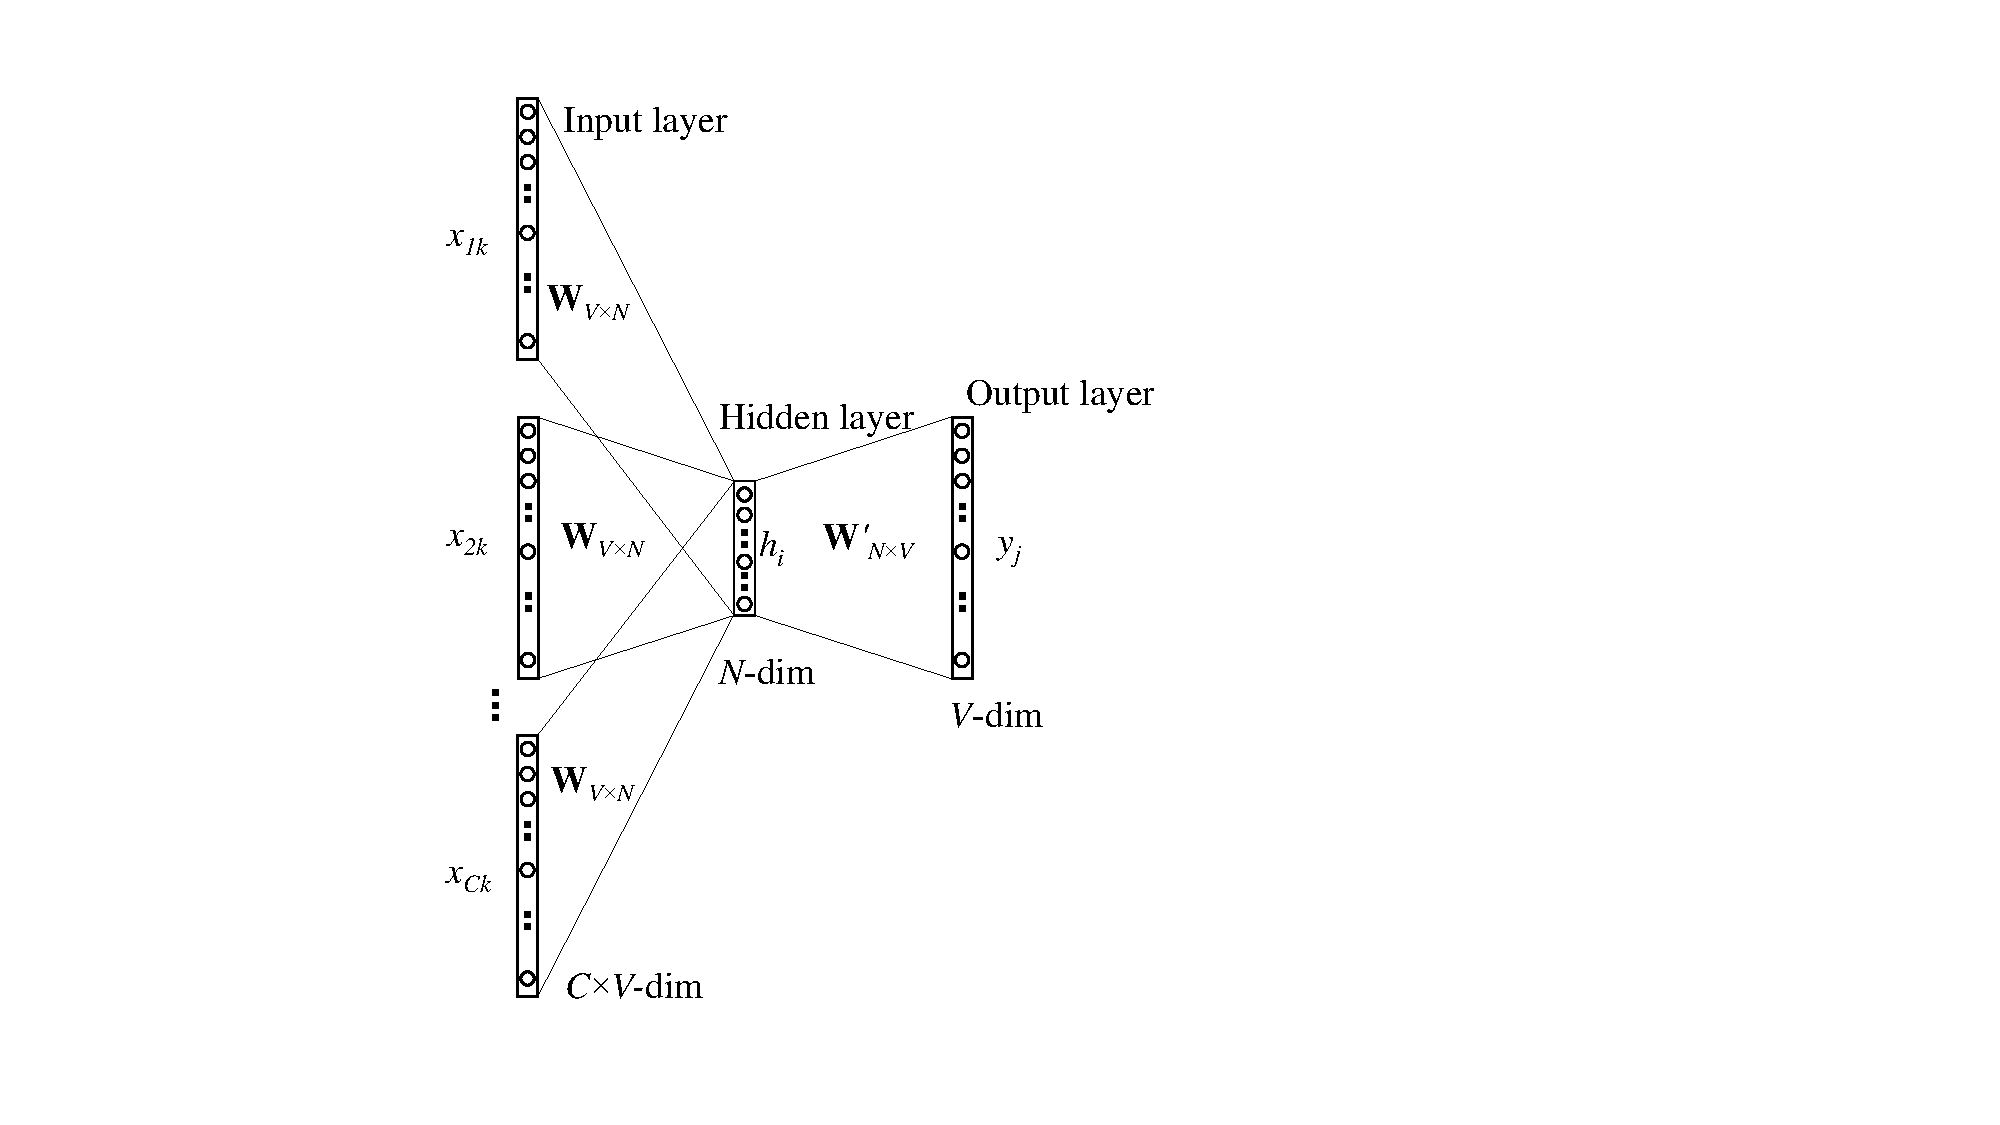
\includegraphics[width=\textwidth]{figures/fig-cbow.pdf}
        \caption{Modelo \acrshort{cbow} de Word2Vec\cite{DBLP:journals/corr/Rong14}\index{Word2Vec}}\label{cbow}
    \end{subfigure}
    \begin{subfigure}[t]{0.4\textwidth}
        \centering
        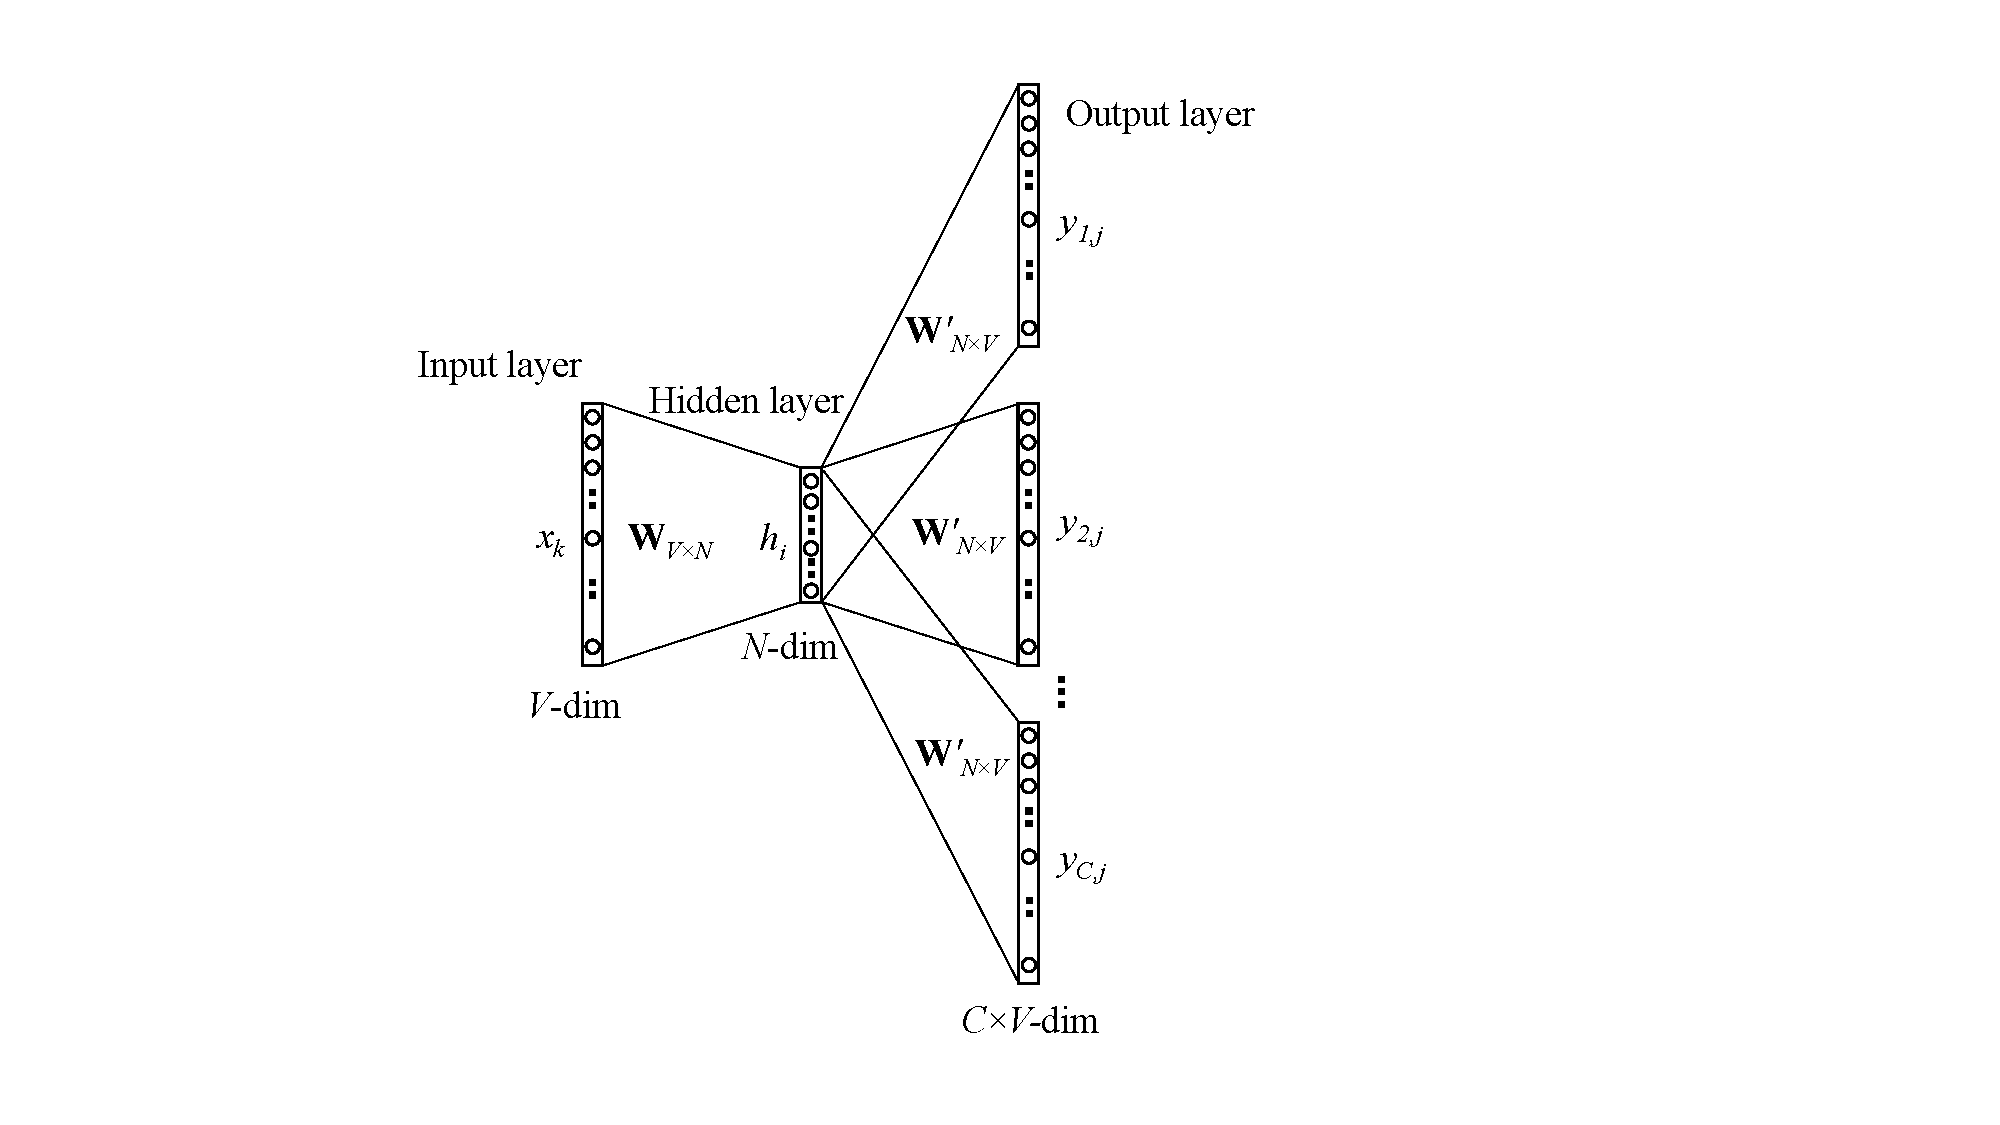
\includegraphics[width=\textwidth]{figures/fig-skip-gram.pdf}
        \caption{Modelo Skip-Gram de Word2Vec\cite{DBLP:journals/corr/Rong14}\index{Word2Vec}}\label{skip-gram}
    \end{subfigure}
    \caption{Modelos Word2Vec\index{Word2Vec}}
\end{figure}

En primer lugar definamos el contexto de las palabras en un corpus. Se elige una ventana de palabras (normalmente un valor entre 2 y 5). Para cada palabra de nuestro corpus creamos parejas de palabras dentro de su ventana por el lado izquierdo y derecho, como se muestra en la tabla~\ref{tab:w2v-window}.

\begin{table}
    \centering
    \begin{tabular}{cp{45mm}}
        \toprule
        Source Text & Training Samples \\
        \midrule
        \colorbox{blue!20}{\colorbox{red!20}{The} quick brown} fox jumps over the lazy dog & (`the', `quick') \newline (`the', `brown') \\
        \midrule
        \colorbox{blue!20}{The \colorbox{red!20}{quick} brown fox} jumps over the lazy dog & (`quick', `the') \newline (`quick', `brown') \newline (`quick', `fox') \\
        \midrule
        \colorbox{blue!20}{The quick \colorbox{red!20}{brown} fox jumps} over the lazy dog & (`brown', `the') \newline (`brown', `quick') \newline (`brown', `fox') \newline (`brown', `jumps') \\
        \midrule
        The \colorbox{blue!20}{quick brown \colorbox{red!20}{fox} jumps over} the lazy dog & (`fox', `quick') \newline (`fox', `brown') \newline (`fox', `jumps') \newline (`fox', `over') \\
        \bottomrule
    \end{tabular}
    \caption{Ventana deslizante en Word2Vec\index{Word2Vec}}\label{tab:w2v-window}
\end{table}

Con las palabras y sus contextos definidos se puede empezar a entrenar nuestro modelo. La figura~\ref{skip-gram} muestra una representación gráfica de la red neuronal que se va a entrenar.

El entrenamiento necesitará 3 capas (input, oculta y output). El número de neuronas en el input y el output será igual al número de palabras en el vocabulario, mientras que el número de neuronas en la capa oculta es un parámetro del modelo que se puede ajustar. Los investigadores que desarrollaron este modelo recomiendan elegir entre 50 y 500 neuronas\cite{DBLP:journals/corr/abs-1301-3781}.

En el input pasarán vectores \gls{one-hot} que representan cada palabra (normalmente en orden alfabético), como se puede ver en la figura~\ref{one-hot}.

\begin{table}
    \centering
    \begin{tabular}{ccc}
        \toprule
        Palabra & Posición por orden alfabético & Vector\\
        \midrule
        fox & 2/3 & [0, 1, 0]\\
        dog & 1/3 & [1, 0, 0]\\
        zebra & 3/3 & [0, 0, 1]\\
        \bottomrule
    \end{tabular}
    \caption{Vectores \gls{one-hot}}\label{one-hot}
\end{table}

Las matrices W y W' se inicializan con unos valores aleatorios, como en cualquier red neuronal. Esta red tiene una función de activación lineal que lo único que hace es pasar a la capa oculta la fila que representa la palabra del input de la matriz W (figura~\ref{h-selection}).

\begin{figure}[!htbp]
    \centering
    \[
        \begin{tikzpicture}[baseline=-0.65ex,scale=0.5]
            \matrix [matrix of math nodes,left delimiter=(,right delimiter=),row sep=0.5cm,column sep=0.5cm] (m) {
                0&0&0&1&0 \\
            };
        \end{tikzpicture}
        \begin{tikzpicture}[baseline=-0.65ex,scale=0.5]
            \matrix [matrix of math nodes,left delimiter=(,right delimiter=),row sep=0.5cm,column sep=0.5cm] (m) {
                17&24&1 \\
                23&5&7 \\
                4&6&13 \\
                10&12&19 \\
                11&18&25 \\
            };
            \draw[color=red] (m-4-1.north west) -- (m-4-1.south west) -- (m-4-3.south east) -- (m-4-3.north east) -- (m-4-1.north west);
        \end{tikzpicture}
        =
        \begin{tikzpicture}[baseline=-0.65ex,scale=0.5]
            \matrix [matrix of math nodes,left delimiter=(,right delimiter=),row sep=0.5cm,column sep=0.5cm] (m) {
                10&12&19 \\
            };
        \end{tikzpicture}
    \]

    \[X_{3} \cdot W_{VxN} = h_{3}\]
    \caption{Función de activación lineal en Word2Vec\index{Word2Vec}}\label{h-selection}
\end{figure}

En el output habrá tantos vectores como hayamos configurado en nuestra ventana (el tamaño del contexto).

\begin{figure}[!htbp]
    \centering
    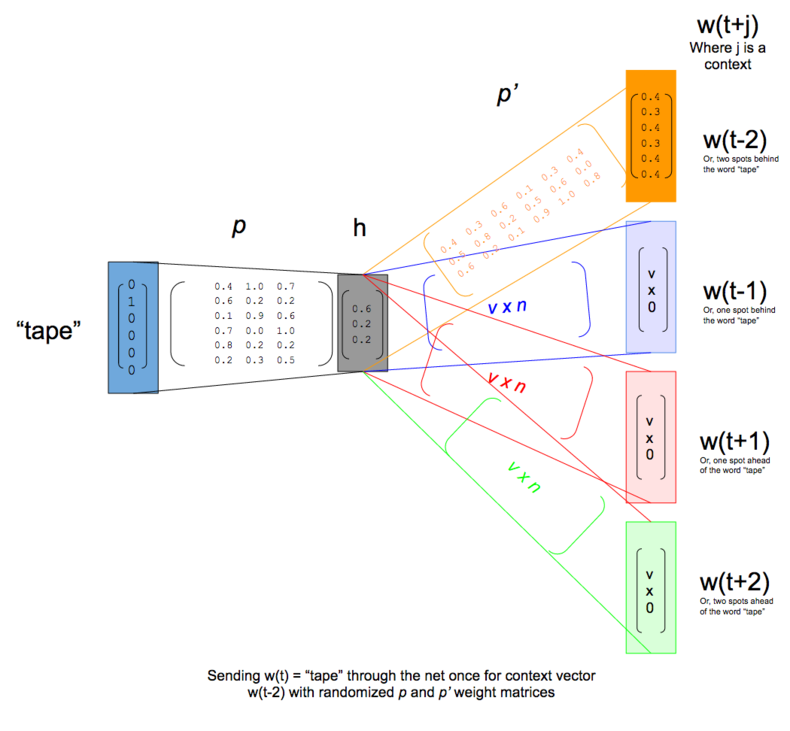
\includegraphics[width=0.8\textwidth]{./figures/skip-gram-exp.png}
    \caption{Representación visual del modelo Skip-Gram\cite{skip-gram-exp}}\label{skip-gram-exp}
\end{figure}

En cada iteración de entrenamiento se siguen los siguientes pasos (la figura~\ref{skip-gram-exp} puede ayudar a visualizar el algoritmo):

\begin{itemize}
    \item Multiplicación de h y W'
    \item Convertir resultado a probabilidades usando \gls{softmax}
    \item Calcular el error entre el resultado y el objetivo (usando los datos reales)
    \item Actualizar pesos en W y W' usando backpropagation
\end{itemize}

Para realizar el cálculo probabilístico se minimiza una funciona de pérdida usando un descenso estocástico\cite{DBLP:journals/corr/Rong14}.

En la práctica, usar softmax con todo el vocabulario no es realista. Para solventar éste problema se usan unas optimizaciones como usar un softmax jerárquico en vez del normal, desechar palabras poco usadas y usar `negative subsampling', entre otras.

La probabilidad de que una palabra se quede en el vocabulario es:

\begin{equation}
    P(w_i) = 1 - \sqrt{\dfrac{t}{f(w_i)}}
\end{equation}

Donde t es un threshold definido por el usuario, $w_i$ una palabra en el corpus y $f(w_i)$

Tras repetir los pasos el número de iteraciones de veces programado la creación del modelo habrá concluido y nuestras probabilidades se encontrarán en la matriz W (en la figura~\ref{skip-gram} entre nuestro vector de entrada y la capa oculta).

Los resultados del modelo son unos vectores para cada palabra de nuestro vocabulario, que se puede comparar con otras para ver su similitud.

\begin{figure}[!htbp]
    \centering
    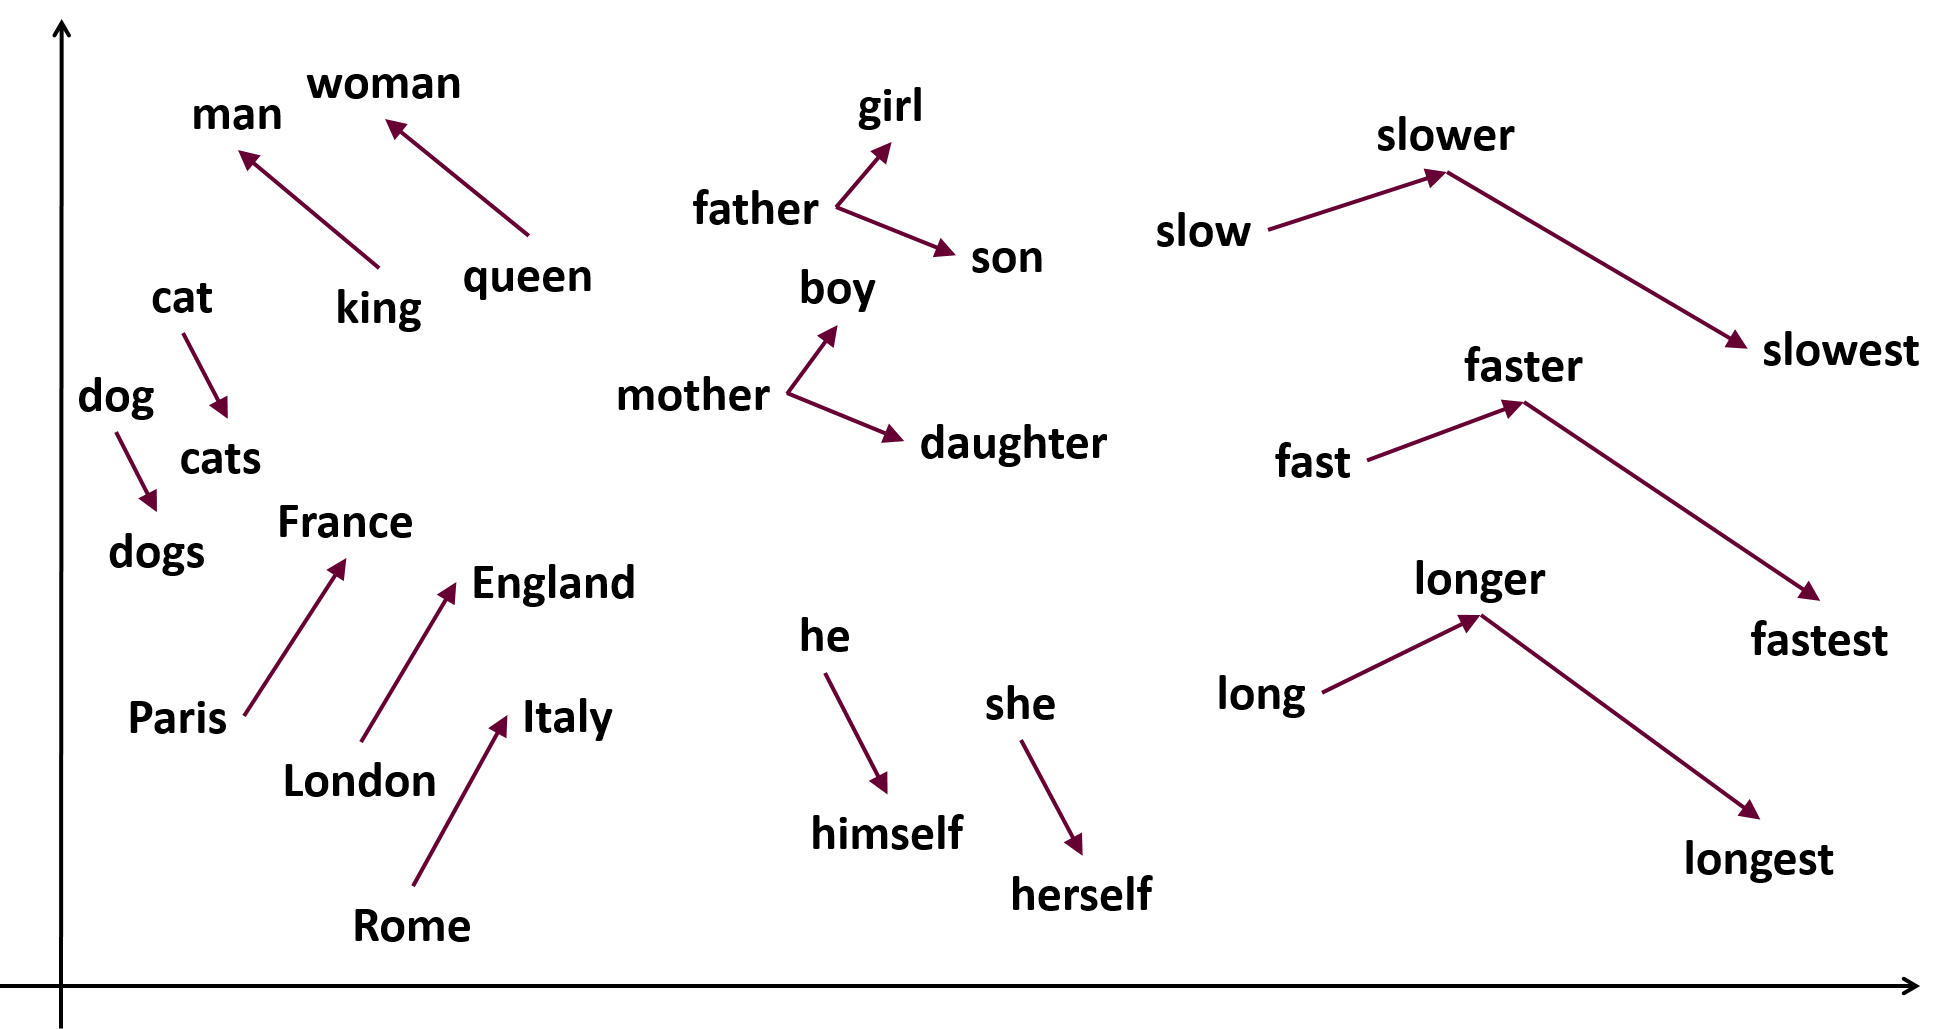
\includegraphics[width=0.7\textwidth]{./figures/res-w2v.png}
    \caption{Vectores de resultado de Word2Vec\index{Word2Vec} en 2D\cite{nlp-gensim}}\label{w2v-general}
\end{figure}

En la tabla~\ref{tab:w2v-res} se pueden ver algunos resultados reales del modelo entrenado con críticas de IMDb\index{IMDb}. La figura~\ref{w2v-general} representa los vectores de un modelo general, visualizado en un plano 2D.

\rowcolors{2}{gray!25}{white}
\begin{table}
    \begin{tabularx}{\textwidth}{XXXXXX}
        \toprule
        \hiderowcolors{}Palabra clave & \multicolumn{5}{c}{Palabras similares}\\
        \midrule
        \showrowcolors{}\textbf{mafia} & dealer & banker & mob & mexican & drug\\
        \textbf{axe} & expedition & undercover & biker & employee & outlaw\\
        \textbf{hair} & clothes & coat & eyes & teeth & makeup\\
        \textbf{airplane} & announcer & sanctuary & engine & accident & ambushed\\
        \textbf{plant} & retrieve & investigate & thwart & unearth & escape\\
        \textbf{air} & automatic & oil & swinging & oxygen & ocean\\
        \bottomrule
    \end{tabularx}
    \caption{Resultados Word2Vec\index{Word2Vec}}\label{tab:w2v-res}
\end{table}

\section{Doc2Vec}
Conceptualmente, Doc2Vec\index{Doc2Vec} es un algoritmo muy similar a Word2Vec\index{Word2Vec}, pero distribuyendo el vocabulario entre varios documentos (o párrafos).

Existen dos modelos diferentes que, de alguna manera, extienden las dos implementaciones de Word2Vec\index{Word2Vec}: Distributed Memory Model \& Distributed Bag of Words. En muchas tareas DBOW funciona mejor, aunque una combinación de los dos modelos da resultados mas consistentes\cite{DBLP:journals/corr/LeM14}.

El Distributed Memory Model se basa en el modelo \acrshort{cbow}, pero añadiendo en el input el id del documento correspondiente y agregando el vector resultante al vector W.

El Distributed Bag of Words Model (figura~\ref{d2v-dbow}) se basa en el modelo Skip-Gram de Word2Vec\index{Word2Vec}. En el input, en vez de aparecer una palabra aparece el id de un documento. La red luego se entrena con un subconjunto de contextos del documento.

\begin{figure}[!htbp]
    \centering
    \begin{subfigure}[t]{0.4\textwidth}
        \centering
        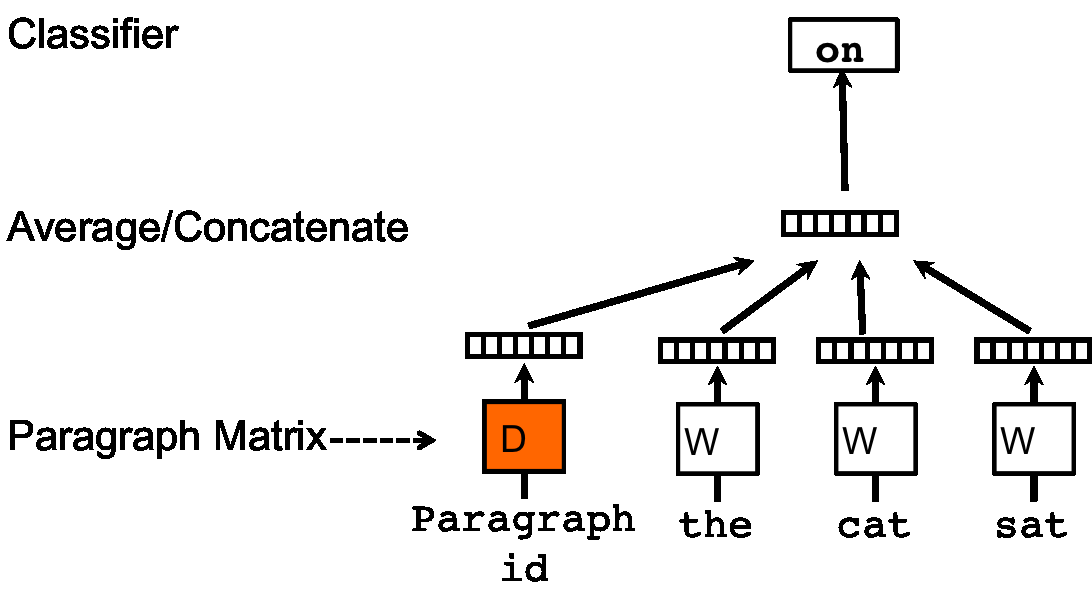
\includegraphics[width=\textwidth]{./figures/distributed_memory_model.pdf}
        \caption{Doc2Vec\index{Doc2Vec} Distributed Memory Model}\label{d2v-dmm}
    \end{subfigure}
    \begin{subfigure}[t]{0.4\textwidth}
        \centering
        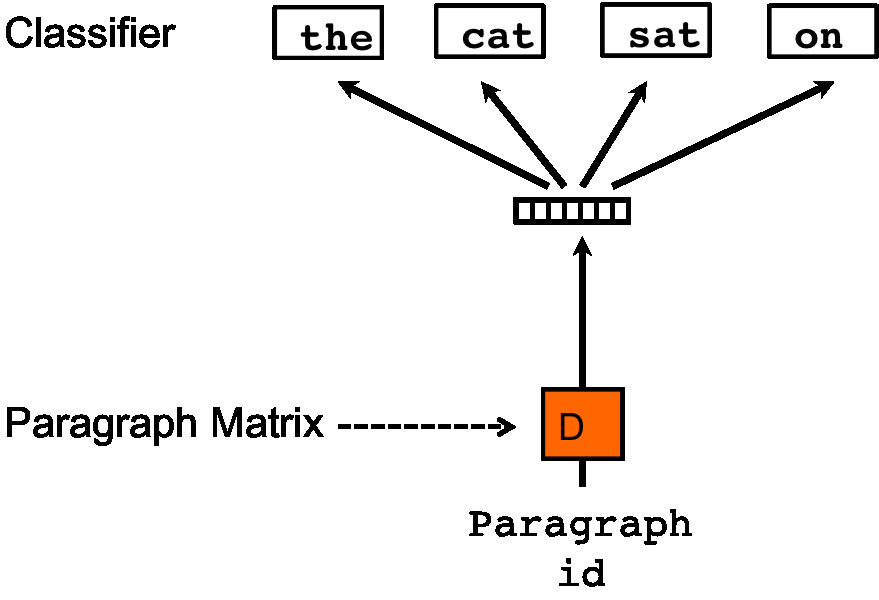
\includegraphics[width=\textwidth]{./figures/distributed_bag_of_words.pdf}
        \caption{Doc2Vec\index{Doc2Vec} Distributed Bag of Words Model}\label{d2v-dbow}
    \end{subfigure}
    \caption{Modelos Doc2Vec\index{Doc2Vec}}
\end{figure}

En ambos casos el resultado del modelo vuelven a ser vectores correspondientes a los documentos con los que se ha entrenado y se pueden hacer las mismas comparaciones que con los vectores de Word2Vec\index{Word2Vec}.

\chapter{E-Modelo}\index{E-Modelo}
E-Modelo\cite{emodelo}\index{E-Modelo} es un algoritmo de recomendación híbrido que intenta aunar el procesamiento de lenguaje natural y los conceptos extraídos de textos con un filtrado colaborativo. Para el filtrado colaborativo se usa \acrfull{als} (la implementación distribuida de Apache Spark\index{Apache Spark}).

En primer lugar es necesario obtener un buen corpus de datos de usuarios y textos. Existen varios datasets como los de Amazon\index{Amazon} y IMDb\index{IMDb}. Para los experimentos realizados se usó un dataset con datos de Amazon\index{Amazon}, pero el algoritmo se podría aplicar a otros ámbitos.

El dataset contiene textos de críticas de usuarios de un producto en particular. Cada producto y cada usuario tiene un identificador único.

Hacemos un procesamiento de los diferentes textos extrayendo palabras clave. El proceso es similar al explicado en el \autoref{chap:clean}.

La matriz del filtrado colaborativo es una matriz tridimensional donde los ejes corresponden a usuarios, productos y palabras.

\begin{figure}[!htbp]
    \begin{tikzpicture}[every node/.style={anchor=north east,fill=white,minimum width=1cm,minimum height=5mm}]
        \matrix (mA) [draw,matrix of math nodes]
        {
            1 & 1 & 0 \\
            0 & 1 & 0 \\
            -1 & -1 & -1 \\
        };

        \matrix (mB) [draw,matrix of math nodes] at ($(mA.south west)+(1.5,0.7)$)
        {
            -1 & -1 & -1 \\
            0 & 2 & 0 \\
            -1 & -1 & -1 \\
        };

        \matrix (mC) [draw,matrix of math nodes] at ($(mB.south west)+(1.5,0.7)$)
        {
            -1 & -1 & -1 \\
            0 & 1 & 0 \\
            0 & 0 & 2 \\
        };

        \node[above=10pt of mA-1-1, rotate=45, yshift=1mm, xshift=8mm] (top-1) {Palabra 1};
        \node[above=10pt of mA-1-2, rotate=45, yshift=1mm, xshift=8mm] (top-2) {Palabra 2};
        \node[above=10pt of mA-1-3, rotate=45, yshift=1mm, xshift=8mm] (top-3) {Palabra 3};

        \node[left=12pt of mC-1-1] (left-1) {Usuario 1};
        \node[left=12pt of mC-2-1] (left-2) {Usuario 2};
        \node[left=12pt of mC-3-1] (left-3) {Usuario 3};

        \node[right=12pt of mC-2-3, yshift=-3mm] (right-1) {Producto 3};
        \node[right=12pt of mB-2-3, yshift=-3mm] (right-2) {Producto 2};
        \node[right=12pt of mA-2-3, yshift=-3mm] (right-3) {Producto 1};

        \draw[dashed](mA.north east)--(mC.north east);
        \draw[dashed](mA.north west)--(mC.north west);
        \draw[dashed](mA.south east)--(mC.south east);
    \end{tikzpicture}
    \caption{Matriz 3D del E-Modelo\index{E-Modelo}}
\end{figure}

Para calcular el resultado de \acrshort{als}\index{ALS} es necesario reducir a dos dimensiones la matriz del E-Modelo\index{E-Modelo}. Para ello pasamos las palabras a columnas, para representar productos-palabra.

\begin{figure}[!htbp]
    \centering
    \vspace*{8mm}
    \begin{tikzpicture}[baseline=-0.65ex,scale=0.8,decoration=brace]
        \matrix [matrix of math nodes,left delimiter=(,right delimiter=),row sep=0.5cm,column sep=0.5cm] (m) {
            1 & 1 & 0 & -1 & -1 & -1 & -1 & -1 & -1 \\
            0 & 1 & 0 & 0 & 2 & 0 & 0 & 1 & 0 \\
            -1 & -1 & -1 & -1 & -1 & -1 & 0 & 0 & 2 \\
        };
        \node[above=10pt of m-1-1, rotate=45, yshift=3mm, xshift=3mm] (top-1) {Palabra 1};
        \node[above=10pt of m-1-2, rotate=45, yshift=3mm, xshift=3mm] (top-2) {Palabra 2};
        \node[above=10pt of m-1-3, rotate=45, yshift=3mm, xshift=3mm] (top-3) {Palabra 3};
        \node[above=10pt of m-1-4, rotate=45, yshift=3mm, xshift=3mm] (top-4) {Palabra 1};
        \node[above=10pt of m-1-5, rotate=45, yshift=3mm, xshift=3mm] (top-5) {Palabra 2};
        \node[above=10pt of m-1-6, rotate=45, yshift=3mm, xshift=3mm] (top-6) {Palabra 3};
        \node[above=10pt of m-1-7, rotate=45, yshift=3mm, xshift=3mm] (top-7) {Palabra 1};
        \node[above=10pt of m-1-8, rotate=45, yshift=3mm, xshift=3mm] (top-8) {Palabra 2};
        \node[above=10pt of m-1-9, rotate=45, yshift=3mm, xshift=3mm] (top-9) {Palabra 3};

        \node[left=20pt of m-1-1] (left-1) {Usuario 1};
        \node[left=20pt of m-2-1] (left-2) {Usuario 2};
        \node[left=15pt of m-3-1] (left-3) {Usuario 3}; % why not aligned?

        \draw[decorate,transform canvas={yshift=2cm},thick] (m-1-1.north west) -- node[above=2pt] {Producto 1} (m-1-3.north east);
        \draw[decorate,transform canvas={yshift=2cm},thick] (m-1-4.north west) -- node[above=2pt] {Producto 2} (m-1-6.north east);
        \draw[decorate,transform canvas={yshift=2cm},thick] (m-1-7.north west) -- node[above=2pt] {Producto 3} (m-1-9.north east);
    \end{tikzpicture}
    \caption{Matriz E-Modelo\index{E-Modelo} de 2 dimensiones}
\end{figure}

Los -1 representan huecos, lo que significa que el usuario no ha escrito una crítica para ese producto en concreto. Los 0 son para palabras del vocabulario que un usuario no ha usado en una de sus crítica.

En matrices más grandes se hace un filtrado posterior para eliminar palabras cuyas columnas sean demasiado dispersas para reducir la cantidad de ceros.

Luego se pasa a un \acrshort{als} normal. Como el calculo de matrices muy grandes es muy elevado se usó un cluster de varios ordenadores para acelerar el análisis.

Antes de crear el modelo final se optimizan probando una serie de parámetros del modelo \acrshort{als}\index{ALS} usando un 10\% de los datos para validación, un 20\% para test y un 70\% para el entrenamiento. Los vectores son escogidos al azar. Una vez probados los parámetros se crea el modelo final con la combinación que mejor resultado dio.

Los parámetros son:

\begin{multicols}{2}
    \begin{itemize}
        \item Rank
        \item Número de iteraciones
        \item Lambda
        \item Seed
    \end{itemize}
\end{multicols}

El resultado es una matriz donde los -1 que había en la matriz original se han convertido en valores estimados. Esos valores representan con que frecuencia un usuario usará una palabra en una crítica de un producto que no ha comprado. Si usamos palabras que describen gustos, como pueden ser los adjetivos calificativos, se puede distinguir cuando una persona va a estar satisfecho con su compra y cuando no.

Resaltar que en este caso la recomendación vendría dada una vez se realiza la predicción de palabras para un usuario y un producto a través de un consiguiente análisis de dichas palabras (por ejemplo, de sentimiento). Este modelo ha sido probado en cuanto a su eficiencia en predicción\cite{emodelo} llegando tener una mejor tasa en precisión cercana al 40\%, pero todavía no es comparable con los ratios de precisión obtenidos en predicción de valoración dado su estado incipiente.

\chapter{Optimización}\label{chap:opt}
Antes de obtener unos resultados definitivos es necesario buscar los mejores parámetros de los diferentes algoritmos. No es fácil evaluar un modelo como éste, ya que no existen unos datos que usar como \textit{`\gls{groundtruth}'}.

Se decidió optimizar el modelo usando películas películas que, a mi parecer, son similares entre sí y analizar que parámetros ajustaban más el resultado. Se ha usado una película de ciencia ficción, una de acción y una de animación infantil.

En las gráficas todos los puntos se han movido lateralmente unos milímetros para que no se solapen en el caso de que su posición sea la misma.

Las líneas en las gráficas se han generado usando una regresión lineal simple para poder ver la tendencia de los modelos más fácilmente.

\section{LSA}
En el modelo \acrshort{lsa}\index{LSA} se pueden ajustar cuatro parámetros.

\begin{itemize}
    \item Minimum Document Frequency: El mínimo número de veces que una palabra debe aparecer en el corpus de documentos para ser usado en el calculo de \acrshort{tfidf}\index{TF-IDF}.
    \item Maximum Document Frequency: Igual que el parámetro anterior, pero para el máximo número de veces que debe aparecer una palabra.
    \item Número de features: Máximo número de features (palabras) en la matriz de \acrshort{tfidf}\index{TF-IDF}. Las palabras menos relevantes se descartán si superan este número.
    \item Número de componentes: Número de dimensiones al que reducir los componentes usando \acrshort{lsa}\index{LSA}
\end{itemize}

Los parámetros elegidos han sido maximum document frequency 200, minimum document frequency 5, número de componentes 1000 y número de features sin límite.

\newlength\figureheight{}
\newlength\figurewidth{}
\setlength\figureheight{0.49\linewidth}
\setlength\figurewidth{\linewidth}
\begin{figure}[!htbp]
    \centering
    % This file was created by matplotlib2tikz v0.6.11.
\begin{tikzpicture}

\definecolor{color0}{rgb}{0,0.833333333333333,1}
\definecolor{color1}{rgb}{1,0.901234567901234,0}

\begin{axis}[
xlabel={Películas},
ylabel={Posición de la recomendación},
xmin=-0.287117890786088, xmax=4.32994465039087,
ymin=0, ymax=205.684972777641,
width=\figurewidth,
height=\figureheight,
xtick={0,1,2,3,4},
xticklabels={Paths of Glory,Full Metal.,Platoon,Saving Private.,The Deer Hunter},
tick align=outside,
xticklabel style = {rotate=45},
tick pos=left,
x grid style={lightgray!92.026143790849673!black},
y grid style={lightgray!92.026143790849673!black},
legend style={at={(0.03,0.97)}, anchor=north west, draw=white!80.0!black},
legend entries={{feat None cmpn 1000 mndf 2 mxdf 100 keyw 0\% lsa 100\% tot 27},{feat None cmpn 1000 mndf 5 mxdf 100 keyw 0\% lsa 100\% tot 37},{feat None cmpn 1000 mndf 10 mxdf 100 keyw 0\% lsa 100\% tot 36},{feat None cmpn 1000 mndf 25 mxdf 100 keyw 0\% lsa 100\% tot 216}},
legend cell align={left}
]
\addplot [only marks, draw=blue!50.0!black, fill=blue!50.0!black, colormap/viridis]
table{%
x                      y
-6.506767982382092e-03 +1.000000000000000e+00
+1.028798272841606e+00 +0.000000000000000e+00
+2.039083089498410e+00 +2.000000000000000e+00
+2.946091620996637e+00 +1.100000000000000e+01
+4.041322966249490e+00 +1.300000000000000e+01
};
\addplot [only marks, draw=color0, fill=color0, colormap/viridis]
table{%
x                      y
-4.999835611280983e-02 +2.000000000000000e+00
+9.883075875519541e-01 +1.000000000000000e+00
+1.950696054107923e+00 +0.000000000000000e+00
+2.975189152393739e+00 +1.100000000000000e+01
+3.934979744325037e+00 +2.300000000000000e+01
};
\addplot [only marks, draw=color1, fill=color1, colormap/viridis]
table{%
x                      y
-4.937729360083317e-03 +2.000000000000000e+00
+1.000695788384633e+00 +1.000000000000000e+00
+1.898381251191249e+00 +0.000000000000000e+00
+3.049655310888514e+00 +1.200000000000000e+01
+3.991536487580606e+00 +2.100000000000000e+01
};
\addplot [only marks, draw=red!50.0!black, fill=red!50.0!black, colormap/viridis]
table{%
x                      y
-4.506292806266332e-02 +1.000000000000000e+00
+9.654247608063696e-01 +5.000000000000000e+00
+1.978674149240178e+00 +7.000000000000000e+00
+2.983042510550827e+00 +9.000000000000000e+00
+4.092515400769211e+00 +1.940000000000000e+02
};
\addplot [semithick, blue!50.0!black, opacity=0.5, forget plot]
table {%
0 -1.6
1 1.9
2 5.4
3 8.9
4 12.4
};
\addplot [semithick, color0, opacity=0.5, forget plot]
table {%
0 -3
1 2.2
2 7.4
3 12.6
4 17.8
};
\addplot [semithick, color1, opacity=0.5, forget plot]
table {%
0 -2.6
1 2.3
2 7.2
3 12.1
4 17
};
\addplot [semithick, red!50.0!black, opacity=0.5, forget plot]
table {%
0 -34.8
1 4.20000000000004
2 43.2
3 82.2000000000001
4 121.2
};
\end{axis}

\end{tikzpicture}
    \caption{Resultados al modificar `Minimum Document Frequency' (Apocalypse Now)}
\end{figure}

\begin{figure}[!htbp]
    \centering
    % This file was created by matplotlib2tikz v0.6.11.
\begin{tikzpicture}

\definecolor{color0}{rgb}{0,0.833333333333333,1}
\definecolor{color1}{rgb}{1,0.901234567901234,0}

\begin{axis}[
xlabel={Películas},
ylabel={Posición de la recomendación},
xmin=-0.555048217005333, xmax=6.47376787913575,
ymin=0, ymax=61.7166789718373,
width=\figurewidth,
height=\figureheight,
xtick={0,1,2,3,4,5,6},
xticklabels={Gravity,Solaris,Interstellar,Alien,The Martian,Planet of the.,Distrito 9},
tick align=outside,
xticklabel style = {rotate=45},
tick pos=left,
x grid style={lightgray!92.026143790849673!black},
y grid style={lightgray!92.026143790849673!black},
legend style={at={(0.03,0.97)}, anchor=north west, draw=white!80.0!black},
legend entries={{feat None cmpn 1000 mndf 2 mxdf 100 keyw 0\% lsa 100\% tot 104},{feat None cmpn 1000 mndf 5 mxdf 100 keyw 0\% lsa 100\% tot 96},{feat None cmpn 1000 mndf 10 mxdf 100 keyw 0\% lsa 100\% tot 107},{feat None cmpn 1000 mndf 25 mxdf 100 keyw 0\% lsa 100\% tot 98}},
legend cell align={left}
]
\addplot [only marks, draw=blue!50.0!black, fill=blue!50.0!black, colormap/viridis]
table{%
x                      y
-2.901836858314227e-02 +1.000000000000000e+00
+1.057713694149493e+00 +5.000000000000000e+00
+2.050493616286072e+00 +1.000000000000000e+01
+3.096119430865328e+00 +9.000000000000000e+00
+4.053406002087733e+00 +1.800000000000000e+01
+4.996310866548055e+00 +2.000000000000000e+01
+6.083821152392776e+00 +4.100000000000000e+01
};
\addplot [only marks, draw=color0, fill=color0, colormap/viridis]
table{%
x                      y
+2.479338055404406e-02 +1.000000000000000e+00
+9.156679045879915e-01 +4.000000000000000e+00
+1.969336957925265e+00 +9.000000000000000e+00
+3.030065099650714e+00 +1.000000000000000e+01
+4.042677535268168e+00 +1.300000000000000e+01
+4.914722671097684e+00 +2.100000000000000e+01
+6.113123241328974e+00 +3.800000000000000e+01
};
\addplot [only marks, draw=color1, fill=color1, colormap/viridis]
table{%
x                      y
+3.909435585580836e-02 +1.000000000000000e+00
+1.121769315296391e+00 +4.000000000000000e+00
+2.073579543378991e+00 +1.000000000000000e+01
+2.957323316209166e+00 +9.000000000000000e+00
+3.965648001014360e+00 +1.200000000000000e+01
+4.975705112529738e+00 +2.700000000000000e+01
+6.062704078488163e+00 +4.400000000000000e+01
};
\addplot [only marks, draw=red!50.0!black, fill=red!50.0!black, colormap/viridis]
table{%
x                      y
-1.941762733128423e-01 +0.000000000000000e+00
+9.662761443476581e-01 +3.000000000000000e+00
+1.956519010079102e+00 +2.000000000000000e+00
+2.980623916736989e+00 +8.000000000000000e+00
+3.915115621512429e+00 +2.100000000000000e+01
+5.006028974367916e+00 +6.000000000000000e+00
+5.893614155532804e+00 +5.800000000000000e+01
};
\addplot [semithick, blue!50.0!black, opacity=0.5, forget plot]
table {%
0 -2.07142857142857
1 3.57142857142858
2 9.21428571428572
3 14.8571428571429
4 20.5
5 26.1428571428571
6 31.7857142857143
};
\addplot [semithick, color0, opacity=0.5, forget plot]
table {%
0 -2.25
1 3.07142857142857
2 8.39285714285714
3 13.7142857142857
4 19.0357142857143
5 24.3571428571429
6 29.6785714285714
};
\addplot [semithick, color1, opacity=0.5, forget plot]
table {%
0 -3.67857142857142
1 2.64285714285715
2 8.96428571428572
3 15.2857142857143
4 21.6071428571429
5 27.9285714285714
6 34.25
};
\addplot [semithick, red!50.0!black, opacity=0.5, forget plot]
table {%
0 -7.32142857142856
1 -0.214285714285706
2 6.89285714285715
3 14
4 21.1071428571429
5 28.2142857142857
6 35.3214285714286
};
\end{axis}

\end{tikzpicture}
    \caption{Resultados al modificar `Minimum Document Frequency' (2001: A Space Odyssey)}
\end{figure}

\begin{figure}[!htbp]
    \centering
    % This file was created by matplotlib2tikz v0.6.11.
\begin{tikzpicture}

\definecolor{color0}{rgb}{0,0.833333333333333,1}
\definecolor{color1}{rgb}{1,0.901234567901234,0}

\begin{axis}[
xlabel={Películas},
ylabel={Posición de la recomendación},
xmin=-0.433584646905039, xmax=5.35236302753746,
ymin=0, ymax=531.863284632035,
width=\figurewidth,
height=\figureheight,
xtick={0,1,2,3,4,5},
xticklabels={Shrek,Monsters\, Inc.,Ponyo,The Incredibles,Toy Story 2,Totoro},
tick align=outside,
xticklabel style = {rotate=45},
tick pos=left,
x grid style={lightgray!92.026143790849673!black},
y grid style={lightgray!92.026143790849673!black},
legend style={at={(0.03,0.97)}, anchor=north west, draw=white!80.0!black},
legend cell align={left},
legend entries={{feat None cmpn 1000 mndf 2 mxdf 100 keyw 0\% lsa 100\% tot 656},{feat None cmpn 1000 mndf 5 mxdf 100 keyw 0\% lsa 100\% tot 504},{feat None cmpn 1000 mndf 10 mxdf 100 keyw 0\% lsa 100\% tot 540},{feat None cmpn 1000 mndf 25 mxdf 100 keyw 0\% lsa 100\% tot 326}}
]
\addplot [only marks, draw=blue!50.0!black, fill=blue!50.0!black, colormap/viridis]
table{%
x                      y
+4.729447977548520e-02 +2.000000000000000e+00
+1.016575492784467e+00 +3.000000000000000e+00
+2.144195707332920e+00 +1.300000000000000e+01
+3.071072675722437e+00 +1.200000000000000e+01
+3.950971985383449e+00 +1.240000000000000e+02
+4.952399019140626e+00 +5.020000000000000e+02
};
\addplot [only marks, draw=color0, fill=color0, colormap/viridis]
table{%
x                      y
+2.748508930605828e-04 +2.000000000000000e+00
+1.088905821801895e+00 +5.000000000000000e+00
+2.056762205283264e+00 +1.400000000000000e+01
+3.018224450825976e+00 +1.300000000000000e+01
+3.901827335271581e+00 +1.580000000000000e+02
+4.943115431438961e+00 +3.120000000000000e+02
};
\addplot [only marks, draw=color1, fill=color1, colormap/viridis]
table{%
x                      y
-1.371013978841097e-01 +2.000000000000000e+00
+1.035347837481359e+00 +6.000000000000000e+00
+1.943244977475858e+00 +9.000000000000000e+00
+3.101896417865547e+00 +1.400000000000000e+01
+3.990618731222936e+00 +1.840000000000000e+02
+5.004418410821604e+00 +3.250000000000000e+02
};
\addplot [only marks, draw=red!50.0!black, fill=red!50.0!black, colormap/viridis]
table{%
x                      y
+6.264955708173160e-02 +2.000000000000000e+00
+1.082597679913373e+00 +1.300000000000000e+01
+2.014569605334113e+00 +1.100000000000000e+01
+3.071460527540011e+00 +1.900000000000000e+01
+4.021998432567651e+00 +3.000000000000000e+01
+5.054712138814764e+00 +2.510000000000000e+02
};
\addplot [semithick, blue!50.0!black, opacity=0.5, forget plot]
table {%
0 -95.0952380952381
1 -13.3238095238096
2 68.447619047619
3 150.219047619048
4 231.990476190476
5 313.761904761905
};
\addplot [semithick, color0, opacity=0.5, forget plot]
table {%
0 -59.4285714285714
1 -2.05714285714287
2 55.3142857142857
3 112.685714285714
4 170.057142857143
5 227.428571428571
};
\addplot [semithick, color1, opacity=0.5, forget plot]
table {%
0 -63.8571428571429
1 -2.31428571428575
2 59.2285714285714
3 120.771428571429
4 182.314285714286
5 243.857142857143
};
\addplot [semithick, red!50.0!black, opacity=0.5, forget plot]
table {%
0 -38.8095238095238
1 -1.55238095238095
2 35.7047619047619
3 72.9619047619047
4 110.219047619048
5 147.47619047619
};
\end{axis}

\end{tikzpicture}

    \caption{Resultados al modificar `Minimum Document Frequency' (Ratatouille)}
\end{figure}

\begin{figure}[!htbp]
    \centering
    % This file was created by matplotlib2tikz v0.6.11.
\begin{tikzpicture}

\definecolor{color0}{rgb}{0,0.833333333333333,1}
\definecolor{color1}{rgb}{1,0.901234567901234,0}

\begin{axis}[
xlabel={Películas},
ylabel={Posición de la recomendación},
xmin=-0.461675873203451, xmax=7.54802900205554,
ymin=0, ymax=468.425568015736,
width=\figurewidth,
height=\figureheight,
xtick={0,1,2,3,4,5,6,7},
xticklabels={Platoon,Full Metal.,Paths of.,Saving.,Das Boot,Fury,Enemy at.,Inglourious.},
tick align=outside,
xticklabel style = {rotate=45},
tick pos=left,
x grid style={lightgray!92.026143790849673!black},
y grid style={lightgray!92.026143790849673!black},
legend style={at={(0.03,0.97)}, anchor=north west, draw=white!80.0!black},
legend cell align={left},
legend entries={{feat None cmpn 1000 mndf 5 mxdf 10 keyw 0\% lsa 100\% tot 760},{feat None cmpn 1000 mndf 5 mxdf 50 keyw 0\% lsa 100\% tot 969},{feat None cmpn 1000 mndf 5 mxdf 100 keyw 0\% lsa 100\% tot 980},{feat None cmpn 1000 mndf 5 mxdf 300 keyw 0\% lsa 100\% tot 1085}}
]
\addplot [only marks, draw=blue!50.0!black, fill=blue!50.0!black, colormap/viridis]
table{%
x                      y
+8.660505913330041e-02 +0.000000000000000e+00
+1.021230881005150e+00 +2.000000000000000e+01
+1.915908149052244e+00 +2.400000000000000e+01
+3.032759720729735e+00 +7.100000000000000e+01
+4.044778834056862e+00 +9.900000000000000e+01
+4.956898348129117e+00 +2.100000000000000e+02
+5.866251335544337e+00 +8.700000000000000e+01
+7.072803902170498e+00 +2.490000000000000e+02
};
\addplot [only marks, draw=color0, fill=color0, colormap/viridis]
table{%
x                      y
-1.477475174115886e-02 +0.000000000000000e+00
+1.071099997897756e+00 +2.000000000000000e+00
+2.062810898964107e+00 +1.000000000000000e+00
+3.084232901956371e+00 +2.900000000000000e+01
+3.942933591835505e+00 +6.600000000000000e+01
+5.011446730057179e+00 +2.390000000000000e+02
+6.062121025962456e+00 +2.100000000000000e+02
+7.120201421534106e+00 +4.220000000000000e+02
};
\addplot [only marks, draw=color1, fill=color1, colormap/viridis]
table{%
x                      y
+1.469887543059621e-01 +0.000000000000000e+00
+9.447654317397486e-01 +1.000000000000000e+00
+1.862344711171062e+00 +2.000000000000000e+00
+2.952166452975252e+00 +1.100000000000000e+01
+4.053689280488338e+00 +1.000000000000000e+02
+5.021631155191365e+00 +1.840000000000000e+02
+5.914866610734476e+00 +4.380000000000000e+02
+7.135850990659610e+00 +2.440000000000000e+02
};
\addplot [only marks, draw=red!50.0!black, fill=red!50.0!black, colormap/viridis]
table{%
x                      y
-4.938867281967018e-02 +0.000000000000000e+00
+8.306366177954851e-01 +4.000000000000000e+00
+2.098189208246438e+00 +1.000000000000000e+00
+2.985512934507834e+00 +4.100000000000000e+01
+3.893781494869969e+00 +9.700000000000000e+01
+4.919291981364379e+00 +2.200000000000000e+02
+5.914694629196947e+00 +3.710000000000000e+02
+7.100592217295436e+00 +3.510000000000000e+02
};
\addplot [semithick, blue!50.0!black, opacity=0.5, forget plot]
table {%
0 -16
1 15.7142857142857
2 47.4285714285714
3 79.1428571428571
4 110.857142857143
5 142.571428571428
6 174.285714285714
7 206
};
\addplot [semithick, color0, opacity=0.5, forget plot]
table {%
0 -76.5833333333334
1 -20.0952380952382
2 36.392857142857
3 92.8809523809523
4 149.369047619047
5 205.857142857143
6 262.345238095238
7 318.833333333333
};
\addplot [semithick, color1, opacity=0.5, forget plot]
table {%
0 -66.1666666666667
1 -12.2619047619048
2 41.6428571428571
3 95.547619047619
4 149.452380952381
5 203.357142857143
6 257.261904761905
7 311.166666666667
};
\addplot [semithick, red!50.0!black, opacity=0.5, forget plot]
table {%
0 -72.9166666666666
1 -13.3333333333333
2 46.25
3 105.833333333333
4 165.416666666667
5 225
6 284.583333333333
7 344.166666666667
};
\end{axis}

\end{tikzpicture}
    \caption{Resultados al modificar `Maximum Document Frequency' (Apocalypse Now)}
\end{figure}

\begin{figure}[!htbp]
    \centering
    % This file was created by matplotlib2tikz v0.6.11.
\begin{tikzpicture}

\definecolor{color0}{rgb}{0,0.833333333333333,1}
\definecolor{color1}{rgb}{1,0.901234567901234,0}

\begin{axis}[
xlabel={Películas},
ylabel={Posición de la recomendación},
xmin=-0.609842492968357, xmax=8.55978077887939,
ymin=0, ymax=216.264444444444,
width=\figurewidth,
height=\figureheight,
xtick={0,1,2,3,4,5,6,7,8},
xticklabels={Gravity,Interstellar,Alien,Planet of.,Distrito 9,Solaris,Close.,The Martian,Aliens},
tick align=outside,
xticklabel style = {rotate=45},
tick pos=left,
x grid style={lightgray!92.026143790849673!black},
y grid style={lightgray!92.026143790849673!black},
legend style={at={(0.91,0.5)}, anchor=east, draw=white!80.0!black},
legend cell align={left},
legend entries={{feat None cmpn 1000 mndf 5 mxdf 10 keyw 0\% lsa 100\% tot 763},{feat None cmpn 1000 mndf 5 mxdf 50 keyw 0\% lsa 100\% tot 117},{feat None cmpn 1000 mndf 5 mxdf 100 keyw 0\% lsa 100\% tot 140},{feat None cmpn 1000 mndf 5 mxdf 300 keyw 0\% lsa 100\% tot 168}}
]
\addplot [only marks, draw=blue!50.0!black, fill=blue!50.0!black, colormap/viridis]
table{%
x                      y
-1.446543383829020e-01 +5.000000000000000e+00
+1.004436943505687e+00 +2.000000000000000e+00
+2.101851742305398e+00 +8.000000000000000e+00
+2.944029242335608e+00 +7.000000000000000e+00
+4.061140284310383e+00 +4.400000000000000e+01
+4.947726058810174e+00 +1.420000000000000e+02
+5.959526683275866e+00 +1.620000000000000e+02
+7.124438957714704e+00 +1.960000000000000e+02
+7.890028125326345e+00 +1.970000000000000e+02
};
\addplot [only marks, draw=color0, fill=color0, colormap/viridis]
table{%
x                      y
-8.778063197938895e-03 +1.000000000000000e+00
+9.407872789299446e-01 +6.000000000000000e+00
+2.046703225078063e+00 +4.000000000000000e+00
+3.021222493440980e+00 +1.700000000000000e+01
+4.004194857933884e+00 +2.300000000000000e+01
+5.014386236193446e+00 +1.500000000000000e+01
+6.049880787221745e+00 +1.600000000000000e+01
+7.032084021065915e+00 +1.000000000000000e+01
+8.088469566358418e+00 +2.500000000000000e+01
};
\addplot [only marks, draw=color1, fill=color1, colormap/viridis]
table{%
x                      y
-3.686963135267912e-02 +1.000000000000000e+00
+9.876171386592587e-01 +9.000000000000000e+00
+1.871490477779731e+00 +1.000000000000000e+01
+2.986248069779700e+00 +2.100000000000000e+01
+4.005369860978845e+00 +3.800000000000000e+01
+4.834923576618640e+00 +4.000000000000000e+00
+5.916822299067301e+00 +1.400000000000000e+01
+6.974540997029592e+00 +1.300000000000000e+01
+7.941318188763412e+00 +3.000000000000000e+01
};
\addplot [only marks, draw=red!50.0!black, fill=red!50.0!black, colormap/viridis]
table{%
x                      y
+1.010574790798213e-01 +1.000000000000000e+00
+1.035796212557589e+00 +3.000000000000000e+00
+2.013075316165445e+00 +1.000000000000000e+01
+3.014173698247239e+00 +2.300000000000000e+01
+3.915172141046385e+00 +3.700000000000000e+01
+4.917002900052351e+00 +0.000000000000000e+00
+5.999814426028440e+00 +1.200000000000000e+01
+7.067761998999949e+00 +1.600000000000000e+01
+8.035290186147229e+00 +6.600000000000000e+01
};
\addplot [semithick, blue!50.0!black, opacity=0.5, forget plot]
table {%
0 -34.7555555555555
1 -4.87222222222215
2 25.0111111111112
3 54.8944444444445
4 84.7777777777778
5 114.661111111111
6 144.544444444444
7 174.427777777778
8 204.311111111111
};
\addplot [semithick, color0, opacity=0.5, forget plot]
table {%
0 4.33333333333333
1 6.5
2 8.66666666666666
3 10.8333333333333
4 13
5 15.1666666666667
6 17.3333333333333
7 19.5
8 21.6666666666667
};
\addplot [semithick, color1, opacity=0.5, forget plot]
table {%
0 7.62222222222222
1 9.60555555555555
2 11.5888888888889
3 13.5722222222222
4 15.5555555555556
5 17.5388888888889
6 19.5222222222222
7 21.5055555555556
8 23.4888888888889
};
\addplot [semithick, red!50.0!black, opacity=0.5, forget plot]
table {%
0 4.736951571734e-15
1 4.66666666666667
2 9.33333333333334
3 14
4 18.6666666666667
5 23.3333333333333
6 28
7 32.6666666666667
8 37.3333333333333
};
\end{axis}

\end{tikzpicture}
    \caption{Resultados al modificar `Maximum Document Frequency' (2001: A Space Odyssey)}
\end{figure}

\begin{figure}[!htbp]
    \centering
    % This file was created by matplotlib2tikz v0.6.11.
\begin{tikzpicture}

\definecolor{color0}{rgb}{0,0.833333333333333,1}
\definecolor{color1}{rgb}{1,0.901234567901234,0}

\begin{axis}[
xlabel={Películas},
ylabel={Posición de la recomendación},
xmin=-0.29385621355134, xmax=5.3615534292556,
ymin=0, ymax=561.260717667749,
width=\figurewidth,
height=\figureheight,
xtick={0,1,2,3,4,5},
xticklabels={The Incredibles,Monsters\, Inc.,Shrek,Ponyo,Toy Story 2,Totoro},
tick align=outside,
xticklabel style = {rotate=45},
tick pos=left,
x grid style={lightgray!92.026143790849673!black},
y grid style={lightgray!92.026143790849673!black},
legend cell align={left},
legend entries={{feat None cmpn 1000 mndf 5 mxdf 10 keyw 0\% lsa 100\% tot 1382},{feat None cmpn 1000 mndf 5 mxdf 50 keyw 0\% lsa 100\% tot 941},{feat None cmpn 1000 mndf 5 mxdf 100 keyw 0\% lsa 100\% tot 504},{feat None cmpn 1000 mndf 5 mxdf 300 keyw 0\% lsa 100\% tot 200}},
legend style={at={(0.03,0.97)}, anchor=north west, draw=white!80.0!black}
]
\addplot [only marks, draw=blue!50.0!black, fill=blue!50.0!black, colormap/viridis]
table{%
x                      y
+5.658183438272429e-02 +4.100000000000000e+01
+9.626340882577124e-01 +1.000000000000000e+02
+2.034364113441558e+00 +2.870000000000000e+02
+3.006153722075286e+00 +3.700000000000000e+02
+3.945113785765690e+00 +3.110000000000000e+02
+4.963326903532982e+00 +2.730000000000000e+02
};
\addplot [only marks, draw=color0, fill=color0, colormap/viridis]
table{%
x                      y
+9.141336593848364e-04 +2.000000000000000e+01
+1.027773163138102e+00 +4.000000000000000e+00
+2.017488136551779e+00 +6.500000000000000e+01
+3.049069684096833e+00 +9.100000000000000e+01
+4.096814139318210e+00 +2.330000000000000e+02
+5.071223225550303e+00 +5.280000000000000e+02
};
\addplot [only marks, draw=color1, fill=color1, colormap/viridis]
table{%
x                      y
+9.270744441497033e-03 +1.300000000000000e+01
+9.546491378855511e-01 +5.000000000000000e+00
+1.936798188014879e+00 +2.000000000000000e+00
+3.031764052516728e+00 +1.400000000000000e+01
+4.034129901821994e+00 +1.580000000000000e+02
+5.047156736082320e+00 +3.120000000000000e+02
};
\addplot [only marks, draw=red!50.0!black, fill=red!50.0!black, colormap/viridis]
table{%
x                      y
-2.615573445126293e-03 +3.900000000000000e+01
+9.084108574746885e-01 +3.100000000000000e+01
+1.951069995380610e+00 +2.400000000000000e+01
+2.984338222644114e+00 +2.700000000000000e+01
+3.976197688903599e+00 +5.600000000000000e+01
+5.026600080802026e+00 +2.300000000000000e+01
};
\addplot [semithick, blue!50.0!black, opacity=0.5, forget plot]
table {%
0 96.3333333333333
1 149.933333333333
2 203.533333333333
3 257.133333333333
4 310.733333333333
5 364.333333333333
};
\addplot [semithick, color0, opacity=0.5, forget plot]
table {%
0 -75.5238095238095
1 17.4190476190476
2 110.361904761905
3 203.304761904762
4 296.247619047619
5 389.190476190476
};
\addplot [semithick, color1, opacity=0.5, forget plot]
table {%
0 -56.4285714285714
1 -0.257142857142867
2 55.9142857142857
3 112.085714285714
4 168.257142857143
5 224.428571428571
};
\addplot [semithick, red!50.0!black, opacity=0.5, forget plot]
table {%
0 33.4761904761905
1 33.4190476190476
2 33.3619047619047
3 33.3047619047619
4 33.247619047619
5 33.1904761904762
};
\end{axis}

\end{tikzpicture}

    \caption{Resultados al modificar `Maximum Document Frequency' (Ratatouille)}
\end{figure}

\begin{figure}[!htbp]
    \centering
    % This file was created by matplotlib2tikz v0.6.11.
\begin{tikzpicture}

\definecolor{color0}{rgb}{0,0.5,1}
\definecolor{color1}{rgb}{0.483870967741935,1,0.483870967741936}
\definecolor{color2}{rgb}{1,0.592592592592593,0}

\begin{axis}[
xlabel={Películas},
ylabel={Posición de la recomendación},
xmin=-0.294554956883588, xmax=4.27941351250573,
ymin=0, ymax=346.518522727273,
width=\figurewidth,
height=\figureheight,
xtick={0,1,2,3,4},
xticklabels={Platoon,Full Metal.,Paths of.,Saving.,The Deer.},
tick align=outside,
xticklabel style = {rotate=45},
tick pos=left,
x grid style={lightgray!92.026143790849673!black},
y grid style={lightgray!92.026143790849673!black},
legend entries={{feat None cmpn 100 mndf 5 mxdf 100 keyw 0\% lsa 100\% tot 339},{feat None cmpn 500 mndf 5 mxdf 100 keyw 0\% lsa 100\% tot 29},{feat None cmpn 1000 mndf 5 mxdf 100 keyw 0\% lsa 100\% tot 37},{feat None cmpn 2000 mndf 5 mxdf 100 keyw 0\% lsa 100\% tot 37},{feat None cmpn 3000 mndf 5 mxdf 100 keyw 0\% lsa 100\% tot 37}},
legend cell align={left},
legend style={at={(0.03,0.97)}, anchor=north west, draw=white!80.0!black}
]
\addplot [only marks, draw=blue!50.0!black, fill=blue!50.0!black, colormap/viridis]
table{%
x                      y
+5.297449651517731e-02 +0.000000000000000e+00
+1.016354705212483e+00 +5.000000000000000e+00
+1.944704481109754e+00 +1.000000000000000e+00
+2.951111055366677e+00 +6.000000000000000e+00
+3.980155300154033e+00 +3.270000000000000e+02
};
\addplot [only marks, draw=color0, fill=color0, colormap/viridis]
table{%
x                      y
-3.097055602261672e-03 +0.000000000000000e+00
+9.999030784811388e-01 +1.000000000000000e+00
+1.986564932589201e+00 +5.000000000000000e+00
+3.003920027956736e+00 +1.400000000000000e+01
+4.044864017709066e+00 +9.000000000000000e+00
};
\addplot [only marks, draw=color1, fill=color1, colormap/viridis]
table{%
x                      y
+1.644067615063349e-02 +0.000000000000000e+00
+9.675437145982385e-01 +1.000000000000000e+00
+2.045845063269300e+00 +2.000000000000000e+00
+2.988757616549518e+00 +1.100000000000000e+01
+4.028546474630483e+00 +2.300000000000000e+01
};
\addplot [only marks, draw=color2, fill=color2, colormap/viridis]
table{%
x                      y
-5.936079179139481e-02 +0.000000000000000e+00
+1.011240126580815e+00 +1.000000000000000e+00
+2.004045598672167e+00 +2.000000000000000e+00
+2.952422677938881e+00 +1.100000000000000e+01
+4.000910349041381e+00 +2.300000000000000e+01
};
\addplot [only marks, draw=red!50.0!black, fill=red!50.0!black, colormap/viridis]
table{%
x                      y
-6.871258986886517e-03 +0.000000000000000e+00
+9.410501494202251e-01 +1.000000000000000e+00
+2.039040515936223e+00 +2.000000000000000e+00
+3.006226656018510e+00 +1.100000000000000e+01
+3.963067890665673e+00 +2.300000000000000e+01
};
\addplot [semithick, blue!50.0!black, opacity=0.5, forget plot]
table {%
0 -63.2
1 2.30000000000004
2 67.8
3 133.3
4 198.8
};
\addplot [semithick, color0, opacity=0.5, forget plot]
table {%
0 -0.399999999999997
1 2.7
2 5.8
3 8.9
4 12
};
\addplot [semithick, color1, opacity=0.5, forget plot]
table {%
0 -3.8
1 1.8
2 7.4
3 13
4 18.6
};
\addplot [semithick, color2, opacity=0.5, forget plot]
table {%
0 -3.8
1 1.8
2 7.4
3 13
4 18.6
};
\addplot [semithick, red!50.0!black, opacity=0.5, forget plot]
table {%
0 -3.8
1 1.8
2 7.4
3 13
4 18.6
};
\end{axis}

\end{tikzpicture}
    \caption{Resultados al modificar `Number of Components' (Apocalypse Now)}
\end{figure}

\begin{figure}[!htbp]
    \centering
    % This file was created by matplotlib2tikz v0.6.11.
\begin{tikzpicture}

\definecolor{color0}{rgb}{0,0.5,1}
\definecolor{color1}{rgb}{0.483870967741935,1,0.483870967741936}
\definecolor{color2}{rgb}{1,0.592592592592593,0}

\begin{axis}[
xlabel={Películas},
ylabel={Posición de la recomendación},
xmin=-0.442737841780122, xmax=6.43473191809422,
ymin=0, ymax=90.9424512987013,
width=\figurewidth,
height=\figureheight,
xtick={0,1,2,3,4,5,6},
xticklabels={Gravity,Solaris,Interstellar,The Martian,Alien,Planet of.,Distrito 9},
tick align=outside,
xticklabel style = {rotate=45},
tick pos=left,
x grid style={lightgray!92.026143790849673!black},
y grid style={lightgray!92.026143790849673!black},
legend cell align={left},
legend style={at={(0.03,0.97)}, anchor=north west, draw=white!80.0!black},
legend entries={{feat None cmpn 100 mndf 5 mxdf 100 keyw 0\% lsa 100\% tot 182},{feat None cmpn 500 mndf 5 mxdf 100 keyw 0\% lsa 100\% tot 115},{feat None cmpn 1000 mndf 5 mxdf 100 keyw 0\% lsa 100\% tot 96},{feat None cmpn 2000 mndf 5 mxdf 100 keyw 0\% lsa 100\% tot 96},{feat None cmpn 3000 mndf 5 mxdf 100 keyw 0\% lsa 100\% tot 96}}
]
\addplot [only marks, draw=blue!50.0!black, fill=blue!50.0!black, colormap/viridis]
table{%
x                      y
-1.060495241312188e-02 +6.000000000000000e+00
+9.407690075318035e-01 +8.000000000000000e+00
+1.897076504771614e+00 +2.000000000000000e+00
+2.899319854527651e+00 +0.000000000000000e+00
+3.977309306393380e+00 +2.100000000000000e+01
+5.015886193229708e+00 +5.900000000000000e+01
+5.948703538260505e+00 +8.600000000000000e+01
};
\addplot [only marks, draw=color0, fill=color0, colormap/viridis]
table{%
x                      y
-8.989422027515323e-02 +1.000000000000000e+00
+1.009337156709079e+00 +2.000000000000000e+00
+2.029160686025713e+00 +1.300000000000000e+01
+3.062914767070549e+00 +1.600000000000000e+01
+4.000918822236569e+00 +9.000000000000000e+00
+4.919071566085274e+00 +2.000000000000000e+01
+6.081888296589256e+00 +5.400000000000000e+01
};
\addplot [only marks, draw=color1, fill=color1, colormap/viridis]
table{%
x                      y
+2.860468805025392e-02 +1.000000000000000e+00
+9.838692564644709e-01 +4.000000000000000e+00
+2.086925817337498e+00 +9.000000000000000e+00
+2.998321730905413e+00 +1.300000000000000e+01
+3.956571498613966e+00 +1.000000000000000e+01
+5.010125559143921e+00 +2.100000000000000e+01
+5.988139042890474e+00 +3.800000000000000e+01
};
\addplot [only marks, draw=color2, fill=color2, colormap/viridis]
table{%
x                      y
+1.995620755089577e-02 +1.000000000000000e+00
+9.694505965890718e-01 +4.000000000000000e+00
+1.945433033206733e+00 +9.000000000000000e+00
+3.030313278747302e+00 +1.300000000000000e+01
+3.996920263024217e+00 +1.000000000000000e+01
+5.106879915224959e+00 +2.100000000000000e+01
+6.050594244968734e+00 +3.800000000000000e+01
};
\addplot [only marks, draw=red!50.0!black, fill=red!50.0!black, colormap/viridis]
table{%
x                      y
+1.085618097766239e-01 +1.000000000000000e+00
+1.027803846315925e+00 +4.000000000000000e+00
+2.112030097491710e+00 +9.000000000000000e+00
+3.114003448431204e+00 +1.300000000000000e+01
+3.936431408964070e+00 +1.000000000000000e+01
+5.073956650311462e+00 +2.100000000000000e+01
+5.969870314201605e+00 +3.800000000000000e+01
};
\addplot [semithick, blue!50.0!black, opacity=0.5, forget plot]
table {%
0 -12.6785714285714
1 0.214285714285724
2 13.1071428571429
3 26
4 38.8928571428571
5 51.7857142857143
6 64.6785714285714
};
\addplot [semithick, color0, opacity=0.5, forget plot]
table {%
0 -4.03571428571428
1 2.78571428571429
2 9.60714285714286
3 16.4285714285714
4 23.25
5 30.0714285714286
6 36.8928571428572
};
\addplot [semithick, color1, opacity=0.5, forget plot]
table {%
0 -1.92857142857142
1 3.28571428571429
2 8.5
3 13.7142857142857
4 18.9285714285714
5 24.1428571428571
6 29.3571428571429
};
\addplot [semithick, color2, opacity=0.5, forget plot]
table {%
0 -1.92857142857142
1 3.28571428571429
2 8.5
3 13.7142857142857
4 18.9285714285714
5 24.1428571428571
6 29.3571428571429
};
\addplot [semithick, red!50.0!black, opacity=0.5, forget plot]
table {%
0 -1.92857142857142
1 3.28571428571429
2 8.5
3 13.7142857142857
4 18.9285714285714
5 24.1428571428571
6 29.3571428571429
};
\end{axis}

\end{tikzpicture}
    \caption{Resultados al modificar `Number of Components' (2001: A Space Odyssey)}
\end{figure}

\begin{figure}[!htbp]
    \centering
    % This file was created by matplotlib2tikz v0.6.11.
\begin{tikzpicture}

\definecolor{color0}{rgb}{0,0.5,1}
\definecolor{color1}{rgb}{0.483870967741935,1,0.483870967741936}
\definecolor{color2}{rgb}{1,0.592592592592593,0}

\begin{axis}[
xlabel={Películas},
ylabel={Posición de la recomendación},
xmin=-0.3618627140013, xmax=5.29814826499389,
ymin=0, ymax=518.922808441558,
width=\figurewidth,
height=\figureheight,
xtick={0,1,2,3,4,5},
xticklabels={Monsters\, Inc.,Shrek,Ponyo,The Incredibles,Toy Story 2,Totoro},
tick align=outside,
xticklabel style = {rotate=45},
tick pos=left,
x grid style={lightgray!92.026143790849673!black},
y grid style={lightgray!92.026143790849673!black},
legend style={at={(0.03,0.97)}, anchor=north west, draw=white!80.0!black},
legend cell align={left},
legend entries={{feat None cmpn 100 mndf 5 mxdf 100 keyw 0\% lsa 100\% tot 705},{feat None cmpn 500 mndf 5 mxdf 100 keyw 0\% lsa 100\% tot 711},{feat None cmpn 1000 mndf 5 mxdf 100 keyw 0\% lsa 100\% tot 504},{feat None cmpn 2000 mndf 5 mxdf 100 keyw 0\% lsa 100\% tot 504},{feat None cmpn 3000 mndf 5 mxdf 100 keyw 0\% lsa 100\% tot 504}}
]
\addplot [only marks, draw=blue!50.0!black, fill=blue!50.0!black, colormap/viridis]
table{%
x                      y
-6.394473233281339e-02 +0.000000000000000e+00
+9.357533877926598e-01 +1.300000000000000e+01
+1.995834962517667e+00 +1.100000000000000e+01
+2.996969550249532e+00 +1.540000000000000e+02
+3.913002038976125e+00 +4.900000000000000e+02
+4.990572592140716e+00 +3.700000000000000e+01
};
\addplot [only marks, draw=color0, fill=color0, colormap/viridis]
table{%
x                      y
+1.586754687863496e-02 +5.000000000000000e+00
+1.120496177329913e+00 +2.000000000000000e+00
+2.042168058169698e+00 +1.400000000000000e+01
+2.942295457440780e+00 +1.300000000000000e+01
+4.005780831707852e+00 +2.290000000000000e+02
+4.977685837851636e+00 +4.480000000000000e+02
};
\addplot [only marks, draw=color1, fill=color1, colormap/viridis]
table{%
x                      y
+2.224594286066601e-02 +5.000000000000000e+00
+9.350124889715326e-01 +2.000000000000000e+00
+2.064615357376006e+00 +1.400000000000000e+01
+3.021740141529022e+00 +1.300000000000000e+01
+3.972217348684087e+00 +1.580000000000000e+02
+4.985793698347377e+00 +3.120000000000000e+02
};
\addplot [only marks, draw=color2, fill=color2, colormap/viridis]
table{%
x                      y
-7.055822972979563e-02 +5.000000000000000e+00
+1.038930866961780e+00 +2.000000000000000e+00
+1.997170192031571e+00 +1.400000000000000e+01
+3.017192270558466e+00 +1.300000000000000e+01
+4.006753323901121e+00 +1.580000000000000e+02
+4.976465802724274e+00 +3.120000000000000e+02
};
\addplot [only marks, draw=red!50.0!black, fill=red!50.0!black, colormap/viridis]
table{%
x                      y
-5.878894397302237e-02 +5.000000000000000e+00
+9.999845596648764e-01 +2.000000000000000e+00
+2.012549615738735e+00 +1.400000000000000e+01
+3.077211308606779e+00 +1.300000000000000e+01
+3.930979895776710e+00 +1.580000000000000e+02
+5.006774568412792e+00 +3.120000000000000e+02
};
\addplot [semithick, blue!50.0!black, opacity=0.5, forget plot]
table {%
0 -8.14285714285718
1 42.1142857142857
2 92.3714285714285
3 142.628571428571
4 192.885714285714
5 243.142857142857
};
\addplot [semithick, color0, opacity=0.5, forget plot]
table {%
0 -88.2857142857142
1 -5.57142857142854
2 77.1428571428572
3 159.857142857143
4 242.571428571429
5 325.285714285714
};
\addplot [semithick, color1, opacity=0.5, forget plot]
table {%
0 -59
1 -1.80000000000001
2 55.4
3 112.6
4 169.8
5 227
};
\addplot [semithick, color2, opacity=0.5, forget plot]
table {%
0 -59
1 -1.80000000000001
2 55.4
3 112.6
4 169.8
5 227
};
\addplot [semithick, red!50.0!black, opacity=0.5, forget plot]
table {%
0 -59
1 -1.80000000000001
2 55.4
3 112.6
4 169.8
5 227
};
\end{axis}

\end{tikzpicture}

    \caption{Resultados al modificar `Number of Components' (Ratatouille)}
\end{figure}

\begin{figure}[!htbp]
    \centering
    % This file was created by matplotlib2tikz v0.6.11.
\begin{tikzpicture}

\definecolor{color0}{rgb}{0.483870967741935,1,0.483870967741936}

\begin{axis}[
xlabel={Películas},
ylabel={Posición de la recomendación},
xmin=-0.283491355170685, xmax=4.30364514661012,
ymin=0, ymax=193.708522727273,
width=\figurewidth,
height=\figureheight,
xtick={0,1,2,3,4},
xticklabels={Paths of.,Full Metal.,Saving.,Platoon,The Deer.},
tick align=outside,
xticklabel style = {rotate=45},
tick pos=left,
x grid style={lightgray!92.026143790849673!black},
y grid style={lightgray!92.026143790849673!black},
legend entries={{feat 2000 cmpn 1000 mndf 5 mxdf 100 keyw 0\% lsa 100\% tot 233},{feat 5000 cmpn 1000 mndf 5 mxdf 100 keyw 0\% lsa 100\% tot 35},{feat None cmpn 1000 mndf 5 mxdf 100 keyw 0\% lsa 100\% tot 37}},
legend style={at={(0.03,0.97)}, anchor=north west, draw=white!80.0!black},
legend cell align={left}
]
\addplot [only marks, draw=blue!50.0!black, fill=blue!50.0!black, colormap/viridis]
table{%
x                      y
-1.094770710767571e-02 +2.000000000000000e+00
+1.017468476072540e+00 +7.000000000000000e+00
+1.995186422591863e+00 +8.000000000000000e+00
+3.013100378141341e+00 +3.300000000000000e+01
+4.070945393596619e+00 +1.830000000000000e+02
};
\addplot [only marks, draw=color0, fill=color0, colormap/viridis]
table{%
x                      y
-4.750546374654548e-02 +2.000000000000000e+00
+9.887907166319483e-01 +1.000000000000000e+00
+1.986315358609423e+00 +1.100000000000000e+01
+2.952746135679334e+00 +0.000000000000000e+00
+4.021598538543233e+00 +2.100000000000000e+01
};
\addplot [only marks, draw=red!50.0!black, fill=red!50.0!black, colormap/viridis]
table{%
x                      y
-4.452508350133422e-02 +2.000000000000000e+00
+1.030268324831481e+00 +1.000000000000000e+00
+2.077366621053750e+00 +1.100000000000000e+01
+2.948765299131759e+00 +0.000000000000000e+00
+3.965898891581123e+00 +2.300000000000000e+01
};
\addplot [semithick, blue!50.0!black, opacity=0.5, forget plot]
table {%
0 -31
1 7.80000000000003
2 46.6
3 85.4
4 124.2
};
\addplot [semithick, color0, opacity=0.5, forget plot]
table {%
0 -0.399999999999998
1 3.3
2 7
3 10.7
4 14.4
};
\addplot [semithick, red!50.0!black, opacity=0.5, forget plot]
table {%
0 -0.8
1 3.3
2 7.4
3 11.5
4 15.6
};
\end{axis}

\end{tikzpicture}
    \caption{Resultados al modificar `Number of Features' (Apocalypse Now)}
\end{figure}

\begin{figure}[!htbp]
    \centering
    % This file was created by matplotlib2tikz v0.6.11.
\begin{tikzpicture}

\definecolor{color0}{rgb}{0.483870967741935,1,0.483870967741936}

\begin{axis}[
xlabel={Películas},
ylabel={Posición de la recomendación},
xmin=-0.433685551148337, xmax=6.3448234626804,
ymin=0, ymax=58.081737012987,
width=\figurewidth,
height=\figureheight,
xtick={0,1,2,3,4,5,6},
xticklabels={Gravity,Solaris,Interstellar,Alien,The Martian,Planet of.,Distrito 9},
tick align=outside,
xticklabel style = {rotate=45},
tick pos=left,
x grid style={lightgray!92.026143790849673!black},
y grid style={lightgray!92.026143790849673!black},
legend entries={{feat 2000 cmpn 1000 mndf 5 mxdf 100 keyw 0\% lsa 100\% tot 137},{feat 5000 cmpn 1000 mndf 5 mxdf 100 keyw 0\% lsa 100\% tot 117},{feat None cmpn 1000 mndf 5 mxdf 100 keyw 0\% lsa 100\% tot 96}},
legend style={at={(0.03,0.97)}, anchor=north west, draw=white!80.0!black},
legend cell align={left}
]
\addplot [only marks, draw=blue!50.0!black, fill=blue!50.0!black, colormap/viridis]
table{%
x                      y
-5.420625617958866e-03 +1.000000000000000e+00
+1.086622088194287e+00 +5.000000000000000e+00
+1.995440067901144e+00 +7.000000000000000e+00
+3.078365322052515e+00 +1.300000000000000e+01
+4.043780263625694e+00 +1.400000000000000e+01
+4.946125615546470e+00 +4.200000000000000e+01
+5.977704951936783e+00 +5.500000000000000e+01
};
\addplot [only marks, draw=color0, fill=color0, colormap/viridis]
table{%
x                      y
-8.528152414794855e-02 +1.000000000000000e+00
+9.718706170388742e-01 +4.000000000000000e+00
+2.107066229334886e+00 +1.000000000000000e+01
+2.922658544319798e+00 +1.100000000000000e+01
+4.069389572958468e+00 +1.300000000000000e+01
+5.083171633766593e+00 +2.700000000000000e+01
+5.979475177772462e+00 +5.100000000000000e+01
};
\addplot [only marks, draw=red!50.0!black, fill=red!50.0!black, colormap/viridis]
table{%
x                      y
-4.725123114241665e-02 +1.000000000000000e+00
+9.359426374888414e-01 +4.000000000000000e+00
+2.052841684428433e+00 +9.000000000000000e+00
+3.055576540820828e+00 +1.000000000000000e+01
+3.924672303573277e+00 +1.300000000000000e+01
+5.152248526925555e+00 +2.100000000000000e+01
+5.995823104116642e+00 +3.800000000000000e+01
};
\addplot [semithick, blue!50.0!black, opacity=0.5, forget plot]
table {%
0 -6.46428571428571
1 2.21428571428572
2 10.8928571428572
3 19.5714285714286
4 28.25
5 36.9285714285714
6 45.6071428571429
};
\addplot [semithick, color0, opacity=0.5, forget plot]
table {%
0 -4.60714285714285
1 2.50000000000001
2 9.60714285714286
3 16.7142857142857
4 23.8214285714286
5 30.9285714285714
6 38.0357142857143
};
\addplot [semithick, red!50.0!black, opacity=0.5, forget plot]
table {%
0 -2.25
1 3.07142857142857
2 8.39285714285714
3 13.7142857142857
4 19.0357142857143
5 24.3571428571429
6 29.6785714285714
};
\end{axis}

\end{tikzpicture}
    \caption{Resultados al modificar `Number of Features' (2001: A Space Odyssey)}
\end{figure}

\begin{figure}[!htbp]
    \centering
    % This file was created by matplotlib2tikz v0.6.11.
\begin{tikzpicture}

\definecolor{color0}{rgb}{0.483870967741935,1,0.483870967741936}

\begin{axis}[
xlabel={Películas},
ylabel={Posición de la recomendación},
xmin=-0.346640451275573, xmax=5.33750705174778,
ymin=0, ymax=346.329951298701,
width=\figurewidth,
height=\figureheight,
xtick={0,1,2,3,4,5},
xticklabels={Shrek,Monsters\, Inc.,Ponyo,The Incredibles,Toy Story 2,Totoro},
tick align=outside,
xticklabel style = {rotate=45},
tick pos=left,
x grid style={lightgray!92.026143790849673!black},
y grid style={lightgray!92.026143790849673!black},
legend style={at={(0.03,0.97)}, anchor=north west, draw=white!80.0!black},
legend entries={{feat 2000 cmpn 1000 mndf 5 mxdf 100 keyw 0\% lsa 100\% tot 578},{feat 5000 cmpn 1000 mndf 5 mxdf 100 keyw 0\% lsa 100\% tot 463},{feat None cmpn 1000 mndf 5 mxdf 100 keyw 0\% lsa 100\% tot 504}},
legend cell align={left}
]
\addplot [only marks, draw=blue!50.0!black, fill=blue!50.0!black, colormap/viridis]
table{%
x                      y
-5.802817474518601e-02 +1.000000000000000e+00
+9.438194535137451e-01 +7.000000000000000e+00
+1.917711120773622e+00 +1.000000000000000e+01
+3.006034283472499e+00 +2.400000000000000e+01
+4.031893351252491e+00 +3.270000000000000e+02
+4.934052430070538e+00 +2.090000000000000e+02
};
\addplot [only marks, draw=color0, fill=color0, colormap/viridis]
table{%
x                      y
+6.366498802012376e-02 +2.000000000000000e+00
+9.992390653301425e-01 +7.000000000000000e+00
+2.010737632320609e+00 +1.300000000000000e+01
+2.970734959804123e+00 +1.700000000000000e+01
+4.003118802453389e+00 +1.710000000000000e+02
+5.027275653882869e+00 +2.530000000000000e+02
};
\addplot [only marks, draw=red!50.0!black, fill=red!50.0!black, colormap/viridis]
table{%
x                      y
+6.635168283415073e-02 +2.000000000000000e+00
+9.788464956280608e-01 +5.000000000000000e+00
+1.987999875649677e+00 +1.400000000000000e+01
+2.888126863936821e+00 +1.300000000000000e+01
+3.945887347519687e+00 +1.580000000000000e+02
+5.044876595228294e+00 +3.120000000000000e+02
};
\addplot [semithick, blue!50.0!black, opacity=0.5, forget plot]
table {%
0 -47.5238095238095
1 10.0190476190476
2 67.5619047619047
3 125.104761904762
4 182.647619047619
5 240.190476190476
};
\addplot [semithick, color0, opacity=0.5, forget plot]
table {%
0 -47.9047619047619
1 2.12380952380954
2 52.152380952381
3 102.180952380952
4 152.209523809524
5 202.238095238095
};
\addplot [semithick, red!50.0!black, opacity=0.5, forget plot]
table {%
0 -59.4285714285714
1 -2.05714285714287
2 55.3142857142857
3 112.685714285714
4 170.057142857143
5 227.428571428571
};
\end{axis}

\end{tikzpicture}

    \caption{Resultados al modificar `Number of Features' (Ratatouille)}
\end{figure}

\section{Doc2Vec}\index{Doc2Vec}
Al igual que en el modelo \acrshort{lsa}, en Doc2Vec\index{Doc2Vec} se pueden ajustar cuatro parámetros.

\begin{itemize}
    \item Size: Número de neuronas (o features) que aprender.
    \item Window: Cuantas palabras usar como ventana para relacionar palabras en una frase. Ejemplo en la figura~\ref{tab:w2v-window}.
    \item Minimum Word Count: Cuantas veces debe aparecer una palabra en nuestro corpus para que pueda ser usada como palabra válida.
    \item Iterations: El número de veces que se entrenará la red neuronal.
\end{itemize}

Los parámetros elegidos han sido size 1000, window 5, minimum count 5 y número de iteraciones 20.

\begin{figure}[!htbp]
    \centering
    % This file was created by matplotlib2tikz v0.6.11.
\begin{tikzpicture}

\definecolor{color0}{rgb}{0,0.833333333333333,1}
\definecolor{color1}{rgb}{1,0.901234567901234,0}

\begin{axis}[
xlabel={Películas},
ylabel={Posición de la recomendación},
xmin=-0.255047915697703, xmax=4.24500146474559,
ymin=0, ymax=8.46870416135204,
width=\figurewidth,
height=\figureheight,
xtick={0,1,2,3,4},
xticklabels={The Deer Hunter,Full Metal.,Platoon,Saving Private.,Paths of Glory},
tick align=outside,
xticklabel style = {rotate=45},
tick pos=left,
x grid style={lightgray!92.026143790849673!black},
y grid style={lightgray!92.026143790849673!black},
legend style={at={(0.03,0.97)}, anchor=north west, draw=white!80.0!black},
legend cell align={left},
legend entries={{size 500 window 8 minc 5 iter 10 tot 16},{size 1000 window 8 minc 5 iter 10 tot 17},{size 2000 window 8 minc 5 iter 10 tot 21},{size 3000 window 8 minc 5 iter 10 tot 17}}
]
\addplot [only marks, draw=blue!50.0!black, fill=blue!50.0!black, colormap/viridis]
table{%
x                      y
-1.744511779645169e-02 +2.000000000000000e+00
+9.441420976335865e-01 +3.000000000000000e+00
+2.019626816798340e+00 +1.000000000000000e+00
+2.941204778517648e+00 +4.000000000000000e+00
+4.013138175136165e+00 +6.000000000000000e+00
};
\addplot [only marks, draw=color0, fill=color0, colormap/viridis]
table{%
x                      y
-2.336190552609479e-02 +0.000000000000000e+00
+1.035778111425212e+00 +3.000000000000000e+00
+1.958678853188445e+00 +1.000000000000000e+00
+3.008013929999184e+00 +7.000000000000000e+00
+4.013315454573978e+00 +6.000000000000000e+00
};
\addplot [only marks, draw=color1, fill=color1, colormap/viridis]
table{%
x                      y
+9.898698561897290e-03 +1.000000000000000e+00
+9.824008938733725e-01 +4.000000000000000e+00
+2.025993823737665e+00 +6.000000000000000e+00
+3.069809457958171e+00 +2.000000000000000e+00
+4.007883086921193e+00 +8.000000000000000e+00
};
\addplot [only marks, draw=red!50.0!black, fill=red!50.0!black, colormap/viridis]
table{%
x                      y
+8.560602518033948e-03 +3.000000000000000e+00
+9.649535466445786e-01 +1.000000000000000e+00
+1.995522437094571e+00 +4.000000000000000e+00
+2.984245985648827e+00 +2.000000000000000e+00
+3.971165930819825e+00 +7.000000000000000e+00
};
\addplot [semithick, blue!50.0!black, opacity=0.5, forget plot]
table {%
0 1.4
1 2.3
2 3.2
3 4.1
4 5
};
\addplot [semithick, color0, opacity=0.5, forget plot]
table {%
0 0.200000000000001
1 1.8
2 3.4
3 5
4 6.6
};
\addplot [semithick, color1, opacity=0.5, forget plot]
table {%
0 1.8
1 3
2 4.2
3 5.4
4 6.6
};
\addplot [semithick, red!50.0!black, opacity=0.5, forget plot]
table {%
0 1.6
1 2.5
2 3.4
3 4.3
4 5.2
};
\end{axis}

\end{tikzpicture}
    \caption{Resultados al modificar `Size' (Apocalypse Now)}
\end{figure}

\begin{figure}[!htbp]
    \centering
    % This file was created by matplotlib2tikz v0.6.11.
\begin{tikzpicture}

\definecolor{color0}{rgb}{0,0.833333333333333,1}
\definecolor{color1}{rgb}{1,0.901234567901234,0}

\begin{axis}[
xlabel={Películas},
ylabel={Posición de la recomendación},
xmin=-0.393559746872722, xmax=6.35507922307891,
ymin=0, ymax=71.1751877029221,
width=\figurewidth,
height=\figureheight,
xtick={0,1,2,3,4,5,6},
xticklabels={Solaris,Interstellar,Distrito 9,Planet of the.,Alien,Gravity,The Martian},
tick align=outside,
xticklabel style = {rotate=45},
tick pos=left,
x grid style={lightgray!92.026143790849673!black},
y grid style={lightgray!92.026143790849673!black},
legend entries={{size 500 window 8 minc 5 iter 10 tot 141},{size 1000 window 8 minc 5 iter 10 tot 138},{size 2000 window 8 minc 5 iter 10 tot 137},{size 3000 window 8 minc 5 iter 10 tot 159}},
legend style={at={(0.03,0.97)}, anchor=north west, draw=white!80.0!black},
legend cell align={left}
]
\addplot [only marks, draw=blue!50.0!black, fill=blue!50.0!black, colormap/viridis]
table{%
x                      y
-5.051310747609351e-02 +0.000000000000000e+00
+9.914487978680301e-01 +1.100000000000000e+01
+2.060019599169483e+00 +1.300000000000000e+01
+3.006977496571128e+00 +1.600000000000000e+01
+3.930859562612881e+00 +1.500000000000000e+01
+4.933081930716490e+00 +2.400000000000000e+01
+6.012032583682283e+00 +6.200000000000000e+01
};
\addplot [only marks, draw=color0, fill=color0, colormap/viridis]
table{%
x                      y
+2.825471145279687e-02 +0.000000000000000e+00
+1.074075761985394e+00 +7.000000000000000e+00
+2.049694508874173e+00 +1.300000000000000e+01
+2.971446126002240e+00 +2.000000000000000e+01
+4.009792653443259e+00 +1.700000000000000e+01
+5.002222959987114e+00 +2.200000000000000e+01
+6.005145532273066e+00 +5.900000000000000e+01
};
\addplot [only marks, draw=color1, fill=color1, colormap/viridis]
table{%
x                      y
-3.977511729427149e-03 +0.000000000000000e+00
+9.609711973322463e-01 +9.000000000000000e+00
+1.910281743776769e+00 +1.000000000000000e+01
+3.063771719246536e+00 +1.300000000000000e+01
+3.966524713191875e+00 +2.100000000000000e+01
+5.025135730410286e+00 +2.400000000000000e+01
+5.897416905374445e+00 +6.000000000000000e+01
};
\addplot [only marks, draw=red!50.0!black, fill=red!50.0!black, colormap/viridis]
table{%
x                      y
+1.415763618725659e-02 +0.000000000000000e+00
+9.151520156721026e-01 +1.100000000000000e+01
+1.942141829791373e+00 +1.300000000000000e+01
+2.900174265289429e+00 +2.100000000000000e+01
+3.982969441308814e+00 +1.900000000000000e+01
+4.949403854150066e+00 +2.800000000000000e+01
+6.002078464208393e+00 +6.700000000000000e+01
};
\addplot [semithick, blue!50.0!black, opacity=0.5, forget plot]
table {%
0 -2.78571428571428
1 4.85714285714287
2 12.5
3 20.1428571428572
4 27.7857142857143
5 35.4285714285714
6 43.0714285714286
};
\addplot [semithick, color0, opacity=0.5, forget plot]
table {%
0 -2.89285714285714
1 4.64285714285715
2 12.1785714285714
3 19.7142857142857
4 27.25
5 34.7857142857143
6 42.3214285714286
};
\addplot [semithick, color1, opacity=0.5, forget plot]
table {%
0 -4.10714285714285
1 3.7857142857143
2 11.6785714285714
3 19.5714285714286
4 27.4642857142857
5 35.3571428571429
6 43.25
};
\addplot [semithick, red!50.0!black, opacity=0.5, forget plot]
table {%
0 -3.10714285714285
1 5.50000000000001
2 14.1071428571429
3 22.7142857142857
4 31.3214285714286
5 39.9285714285714
6 48.5357142857143
};
\end{axis}

\end{tikzpicture}
    \caption{Resultados al modificar `Size' (2001: A Space Odyssey)}
\end{figure}

\begin{figure}[!htbp]
    \centering
    % This file was created by matplotlib2tikz v0.6.11.
\begin{tikzpicture}

\definecolor{color0}{rgb}{0,0.833333333333333,1}
\definecolor{color1}{rgb}{1,0.901234567901234,0}

\begin{axis}[
xlabel={Películas},
ylabel={Posición de la recomendación},
xmin=-0.383723180838573, xmax=5.32674150024266,
ymin=0, ymax=38.9918560606061,
width=\figurewidth,
height=\figureheight,
xtick={0,1,2,3,4,5},
xticklabels={The Incredibles,Ponyo,Totoro,Monsters\, Inc.,Toy Story 2,Shrek},
tick align=outside,
xticklabel style = {rotate=45},
tick pos=left,
x grid style={lightgray!92.026143790849673!black},
y grid style={lightgray!92.026143790849673!black},
legend entries={{size 500 window 8 minc 5 iter 10 tot 108},{size 1000 window 8 minc 5 iter 10 tot 93},{size 2000 window 8 minc 5 iter 10 tot 101},{size 3000 window 8 minc 5 iter 10 tot 98}},
legend style={at={(0.03,0.97)}, anchor=north west, draw=white!80.0!black},
legend cell align={left}
]
\addplot [only marks, draw=blue!50.0!black, fill=blue!50.0!black, colormap/viridis]
table{%
x                      y
+9.689006952537179e-03 +0.000000000000000e+00
+1.040890176408114e+00 +8.000000000000000e+00
+1.995338296012762e+00 +1.100000000000000e+01
+3.016822392067824e+00 +2.300000000000000e+01
+3.902941650976415e+00 +2.900000000000000e+01
+4.993442530183200e+00 +3.700000000000000e+01
};
\addplot [only marks, draw=color0, fill=color0, colormap/viridis]
table{%
x                      y
-9.059615402084031e-02 +0.000000000000000e+00
+1.036449082768617e+00 +9.000000000000000e+00
+2.040668259955923e+00 +1.300000000000000e+01
+2.952198634671171e+00 +1.900000000000000e+01
+3.950388132075631e+00 +2.300000000000000e+01
+5.033614473424930e+00 +2.900000000000000e+01
};
\addplot [only marks, draw=color1, fill=color1, colormap/viridis]
table{%
x                      y
-5.078612384315343e-02 +1.000000000000000e+00
+1.035600372836946e+00 +1.000000000000000e+01
+2.033306522725435e+00 +7.000000000000000e+00
+3.025432013835106e+00 +2.300000000000000e+01
+4.017126034344734e+00 +2.800000000000000e+01
+5.000789056322449e+00 +3.200000000000000e+01
};
\addplot [only marks, draw=red!50.0!black, fill=red!50.0!black, colormap/viridis]
table{%
x                      y
-5.497883336608279e-02 +1.000000000000000e+00
+9.962952783012485e-01 +4.000000000000000e+00
+1.972620603182140e+00 +7.000000000000000e+00
+3.055670484591426e+00 +2.000000000000000e+01
+4.067327772303507e+00 +3.000000000000000e+01
+4.962318343319420e+00 +3.600000000000000e+01
};
\addplot [semithick, blue!50.0!black, opacity=0.5, forget plot]
table {%
0 -0.571428571428571
1 6.85714285714285
2 14.2857142857143
3 21.7142857142857
4 29.1428571428571
5 36.5714285714286
};
\addplot [semithick, color0, opacity=0.5, forget plot]
table {%
0 1.71428571428571
1 7.22857142857143
2 12.7428571428571
3 18.2571428571428
4 23.7714285714286
5 29.2857142857143
};
\addplot [semithick, color1, opacity=0.5, forget plot]
table {%
0 0.761904761904762
1 7.19047619047619
2 13.6190476190476
3 20.047619047619
4 26.4761904761905
5 32.9047619047619
};
\addplot [semithick, red!50.0!black, opacity=0.5, forget plot]
table {%
0 -2.66666666666667
1 4.93333333333333
2 12.5333333333333
3 20.1333333333333
4 27.7333333333333
5 35.3333333333333
};
\end{axis}

\end{tikzpicture}

    \caption{Resultados al modificar `Size' (Ratatouille)}
\end{figure}

\begin{figure}[!htbp]
    \centering
    % This file was created by matplotlib2tikz v0.6.11.
\begin{tikzpicture}

\definecolor{color0}{rgb}{0,0.833333333333333,1}
\definecolor{color1}{rgb}{1,0.901234567901234,0}

\begin{axis}[
xlabel={Películas},
ylabel={Posición de la recomendación},
xmin=-0.248779429241788, xmax=4.34855611461577,
ymin=0, ymax=10.5849330357143,
width=\figurewidth,
height=\figureheight,
xtick={0,1,2,3,4},
xticklabels={Saving Private.,Full Metal.,Platoon,The Deer Hunter,Paths of Glory},
tick align=outside,
xticklabel style = {rotate=45},
tick pos=left,
x grid style={lightgray!92.026143790849673!black},
y grid style={lightgray!92.026143790849673!black},
legend entries={{size 1000 window 3 minc 5 iter 10 tot 21},{size 1000 window 5 minc 5 iter 10 tot 19},{size 1000 window 8 minc 5 iter 10 tot 20},{size 1000 window 10 minc 5 iter 10 tot 26}},
legend cell align={left},
legend style={at={(0.03,0.97)}, anchor=north west, draw=white!80.0!black}
]
\addplot [only marks, draw=blue!50.0!black, fill=blue!50.0!black, colormap/viridis]
table{%
x                      y
-1.561608340662048e-02 +3.000000000000000e+00
+1.003665089608013e+00 +0.000000000000000e+00
+2.009307730171247e+00 +2.000000000000000e+00
+3.006187553582918e+00 +9.000000000000000e+00
+4.003097870937568e+00 +7.000000000000000e+00
};
\addplot [only marks, draw=color0, fill=color0, colormap/viridis]
table{%
x                      y
-4.179225575674087e-03 +1.000000000000000e+00
+1.010112721679326e+00 +5.000000000000000e+00
+1.986511139295239e+00 +2.000000000000000e+00
+3.017916601213269e+00 +3.000000000000000e+00
+3.973018796315184e+00 +8.000000000000000e+00
};
\addplot [only marks, draw=color1, fill=color1, colormap/viridis]
table{%
x                      y
+7.306963403913465e-02 +1.000000000000000e+00
+1.007198285956633e+00 +3.000000000000000e+00
+2.073274399901223e+00 +6.000000000000000e+00
+3.029562513432524e+00 +2.000000000000000e+00
+4.112526975496956e+00 +8.000000000000000e+00
};
\addplot [only marks, draw=red!50.0!black, fill=red!50.0!black, colormap/viridis]
table{%
x                      y
+1.866219923395850e-02 +5.000000000000000e+00
+9.975030550275386e-01 +3.000000000000000e+00
+2.056906041999223e+00 +6.000000000000000e+00
+2.971712260062434e+00 +2.000000000000000e+00
+3.983171678877306e+00 +1.000000000000000e+01
};
\addplot [semithick, blue!50.0!black, opacity=0.5, forget plot]
table {%
0 0.800000000000001
1 2.5
2 4.2
3 5.9
4 7.6
};
\addplot [semithick, color0, opacity=0.5, forget plot]
table {%
0 1.4
1 2.6
2 3.8
3 5
4 6.2
};
\addplot [semithick, color1, opacity=0.5, forget plot]
table {%
0 1.4
1 2.7
2 4
3 5.3
4 6.6
};
\addplot [semithick, red!50.0!black, opacity=0.5, forget plot]
table {%
0 3.4
1 4.3
2 5.2
3 6.1
4 7
};
\end{axis}

\end{tikzpicture}
    \caption{Resultados al modificar `Window' (Apocalypse Now)}
\end{figure}

\begin{figure}[!htbp]
    \centering
    % This file was created by matplotlib2tikz v0.6.11.
\begin{tikzpicture}

\definecolor{color0}{rgb}{0,0.833333333333333,1}
\definecolor{color1}{rgb}{1,0.901234567901234,0}

\begin{axis}[
xlabel={Películas},
ylabel={Posición de la recomendación},
xmin=-0.407733023228943, xmax=6.46414904806693,
ymin=0, ymax=81.8391458882914,
width=\figurewidth,
height=\figureheight,
xtick={0,1,2,3,4,5,6},
xticklabels={Solaris,Interstellar,Distrito 9,Planet of the.,Alien,Gravity,The Martian},
tick align=outside,
xticklabel style = {rotate=45},
tick pos=left,
x grid style={lightgray!92.026143790849673!black},
y grid style={lightgray!92.026143790849673!black},
legend cell align={left},
legend style={at={(0.03,0.97)}, anchor=north west, draw=white!80.0!black},
legend entries={{size 1000 window 3 minc 5 iter 10 tot 129},{size 1000 window 5 minc 5 iter 10 tot 111},{size 1000 window 8 minc 5 iter 10 tot 143},{size 1000 window 10 minc 5 iter 10 tot 163}}
]
\addplot [only marks, draw=blue!50.0!black, fill=blue!50.0!black, colormap/viridis]
table{%
x                      y
+3.506846797043030e-02 +0.000000000000000e+00
+9.817581206778054e-01 +9.000000000000000e+00
+1.900039319227744e+00 +1.600000000000000e+01
+2.972896629068051e+00 +1.100000000000000e+01
+4.014181472363457e+00 +8.000000000000000e+00
+4.950734114600046e+00 +2.600000000000000e+01
+6.053107328800729e+00 +5.900000000000000e+01
};
\addplot [only marks, draw=color0, fill=color0, colormap/viridis]
table{%
x                      y
+1.358059926847923e-03 +0.000000000000000e+00
+9.665157776728900e-01 +1.100000000000000e+01
+1.938385264546487e+00 +1.600000000000000e+01
+2.997964059782109e+00 +1.000000000000000e+01
+4.085108167334652e+00 +1.700000000000000e+01
+5.044467882064920e+00 +2.100000000000000e+01
+6.034366658357040e+00 +3.600000000000000e+01
};
\addplot [only marks, draw=color1, fill=color1, colormap/viridis]
table{%
x                      y
+5.723640351712631e-02 +0.000000000000000e+00
+1.065848370403365e+00 +7.000000000000000e+00
+1.956608785440840e+00 +1.000000000000000e+01
+2.934118262926154e+00 +2.000000000000000e+01
+3.972813047696823e+00 +2.200000000000000e+01
+5.124773606719176e+00 +1.400000000000000e+01
+6.089952328607143e+00 +7.000000000000000e+01
};
\addplot [only marks, draw=red!50.0!black, fill=red!50.0!black, colormap/viridis]
table{%
x                      y
-5.432506763021979e-02 +0.000000000000000e+00
+9.834196511509600e-01 +9.000000000000000e+00
+2.088062171591054e+00 +1.300000000000000e+01
+3.010015936142026e+00 +2.000000000000000e+01
+4.077112939890906e+00 +1.800000000000000e+01
+5.026803720925459e+00 +2.600000000000000e+01
+6.110741092468205e+00 +7.700000000000000e+01
};
\addplot [semithick, blue!50.0!black, opacity=0.5, forget plot]
table {%
0 -3.32142857142857
1 3.92857142857143
2 11.1785714285714
3 18.4285714285714
4 25.6785714285714
5 32.9285714285714
6 40.1785714285714
};
\addplot [semithick, color0, opacity=0.5, forget plot]
table {%
0 2.03571428571429
1 6.64285714285714
2 11.25
3 15.8571428571429
4 20.4642857142857
5 25.0714285714286
6 29.6785714285714
};
\addplot [semithick, color1, opacity=0.5, forget plot]
table {%
0 -4.85714285714285
1 3.57142857142858
2 12
3 20.4285714285714
4 28.8571428571429
5 37.2857142857143
6 45.7142857142857
};
\addplot [semithick, red!50.0!black, opacity=0.5, forget plot]
table {%
0 -5.64285714285714
1 4.00000000000001
2 13.6428571428571
3 23.2857142857143
4 32.9285714285714
5 42.5714285714286
6 52.2142857142857
};
\end{axis}

\end{tikzpicture}
    \caption{Resultados al modificar `Window' (2001: A Space Odyssey)}
\end{figure}

\begin{figure}[!htbp]
    \centering
    % This file was created by matplotlib2tikz v0.6.11.
\begin{tikzpicture}

\definecolor{color0}{rgb}{0,0.833333333333333,1}
\definecolor{color1}{rgb}{1,0.901234567901234,0}

\begin{axis}[
xlabel={Películas},
ylabel={Posición de la recomendación},
xmin=-0.309373984768796, xmax=5.35278439809052,
ymin=0, ymax=47.805955762987,
width=\figurewidth,
height=\figureheight,
xtick={0,1,2,3,4,5},
xticklabels={The Incredibles,Ponyo,Totoro,Monsters\, Inc.,Toy Story 2,Shrek},
tick align=outside,
xticklabel style = {rotate=45},
tick pos=left,
x grid style={lightgray!92.026143790849673!black},
y grid style={lightgray!92.026143790849673!black},
legend entries={{size 1000 window 3 minc 5 iter 10 tot 127},{size 1000 window 5 minc 5 iter 10 tot 111},{size 1000 window 8 minc 5 iter 10 tot 97},{size 1000 window 10 minc 5 iter 10 tot 97}},
legend cell align={left},
legend style={at={(0.03,0.97)}, anchor=north west, draw=white!80.0!black}
]
\addplot [only marks, draw=blue!50.0!black, fill=blue!50.0!black, colormap/viridis]
table{%
x                      y
-5.314525150271352e-03 +2.000000000000000e+00
+1.010569522809533e+00 +1.500000000000000e+01
+2.012145988922724e+00 +1.200000000000000e+01
+3.027916180186197e+00 +2.400000000000000e+01
+3.976894933725483e+00 +3.100000000000000e+01
+5.014384706280669e+00 +4.300000000000000e+01
};
\addplot [only marks, draw=color0, fill=color0, colormap/viridis]
table{%
x                      y
+7.914636804475350e-02 +1.000000000000000e+00
+8.606538579499989e-01 +3.000000000000000e+00
+2.039505179346953e+00 +8.000000000000000e+00
+2.984791382044105e+00 +2.900000000000000e+01
+3.978553609319218e+00 +2.500000000000000e+01
+5.061613957187628e+00 +4.500000000000000e+01
};
\addplot [only marks, draw=color1, fill=color1, colormap/viridis]
table{%
x                      y
-1.786564701419568e-02 +2.000000000000000e+00
+9.678773252714697e-01 +4.000000000000000e+00
+1.969624636805386e+00 +7.000000000000000e+00
+2.988094308330262e+00 +2.100000000000000e+01
+4.049804841352701e+00 +2.600000000000000e+01
+4.968075077021312e+00 +3.700000000000000e+01
};
\addplot [only marks, draw=red!50.0!black, fill=red!50.0!black, colormap/viridis]
table{%
x                      y
+4.301924639712805e-02 +0.000000000000000e+00
+1.023506124561892e+00 +5.000000000000000e+00
+2.022127774276788e+00 +9.000000000000000e+00
+3.037053359413724e+00 +2.300000000000000e+01
+4.034742962932957e+00 +2.700000000000000e+01
+5.023964221361378e+00 +3.300000000000000e+01
};
\addplot [semithick, blue!50.0!black, opacity=0.5, forget plot]
table {%
0 2.23809523809524
1 9.8095238095238
2 17.3809523809524
3 24.9523809523809
4 32.5238095238095
5 40.0952380952381
};
\addplot [semithick, color0, opacity=0.5, forget plot]
table {%
0 -3.42857142857143
1 5.34285714285714
2 14.1142857142857
3 22.8857142857143
4 31.6571428571428
5 40.4285714285714
};
\addplot [semithick, color1, opacity=0.5, forget plot]
table {%
0 -2.04761904761905
1 5.23809523809524
2 12.5238095238095
3 19.8095238095238
4 27.0952380952381
5 34.3809523809524
};
\addplot [semithick, red!50.0!black, opacity=0.5, forget plot]
table {%
0 -1.33333333333333
1 5.66666666666667
2 12.6666666666667
3 19.6666666666667
4 26.6666666666667
5 33.6666666666667
};
\end{axis}

\end{tikzpicture}

    \caption{Resultados al modificar `Window' (Ratatouille)}
\end{figure}

\begin{figure}[!htbp]
    \centering
    % This file was created by matplotlib2tikz v0.6.11.
\begin{tikzpicture}

\definecolor{color0}{rgb}{0,0.833333333333333,1}
\definecolor{color1}{rgb}{1,0.901234567901234,0}

\begin{axis}[
xlabel={Películas},
ylabel={Posición de la recomendación},
xmin=-0.297823785511582, xmax=4.28721281313969,
ymin=0, ymax=7.41942063934949,
width=\figurewidth,
height=\figureheight,
xtick={0,1,2,3,4},
xticklabels={Saving Private.,Full Metal.,The Deer Hunter,Platoon,Paths of Glory},
tick align=outside,
xticklabel style = {rotate=45},
tick pos=left,
x grid style={lightgray!92.026143790849673!black},
y grid style={lightgray!92.026143790849673!black},
legend style={at={(0.03,0.97)}, anchor=north west, draw=white!80.0!black},
legend cell align={left},
legend entries={{size 1000 window 5 minc 2 iter 10 tot 19},{size 1000 window 5 minc 5 iter 10 tot 15},{size 1000 window 5 minc 7 iter 10 tot 19},{size 1000 window 5 minc 10 iter 10 tot 22}}
]
\addplot [only marks, draw=blue!50.0!black, fill=blue!50.0!black, colormap/viridis]
table{%
x                      y
-4.565173176697534e-02 +3.000000000000000e+00
+1.088817651610832e+00 +0.000000000000000e+00
+2.066319660139641e+00 +4.000000000000000e+00
+3.003628498270540e+00 +5.000000000000000e+00
+3.970530652217362e+00 +7.000000000000000e+00
};
\addplot [only marks, draw=color0, fill=color0, colormap/viridis]
table{%
x                      y
-2.458988562963605e-02 +0.000000000000000e+00
+9.854322185369808e-01 +4.000000000000000e+00
+1.976630304684926e+00 +2.000000000000000e+00
+3.008629914714495e+00 +3.000000000000000e+00
+3.999214662206199e+00 +6.000000000000000e+00
};
\addplot [only marks, draw=color1, fill=color1, colormap/viridis]
table{%
x                      y
-6.216050302618101e-02 +1.000000000000000e+00
+9.658624876991605e-01 +3.000000000000000e+00
+2.062566565676021e+00 +4.000000000000000e+00
+3.040772916907657e+00 +5.000000000000000e+00
+4.042820315069653e+00 +6.000000000000000e+00
};
\addplot [only marks, draw=red!50.0!black, fill=red!50.0!black, colormap/viridis]
table{%
x                      y
-3.683922560935416e-02 +3.000000000000000e+00
+9.794674415739469e-01 +4.000000000000000e+00
+2.046539380320710e+00 +2.000000000000000e+00
+2.945198338161063e+00 +6.000000000000000e+00
+4.051128059896423e+00 +7.000000000000000e+00
};
\addplot [semithick, blue!50.0!black, opacity=0.5, forget plot]
table {%
0 1.2
1 2.5
2 3.8
3 5.1
4 6.4
};
\addplot [semithick, color0, opacity=0.5, forget plot]
table {%
0 0.800000000000001
1 1.9
2 3
3 4.1
4 5.2
};
\addplot [semithick, color1, opacity=0.5, forget plot]
table {%
0 1.4
1 2.6
2 3.8
3 5
4 6.2
};
\addplot [semithick, red!50.0!black, opacity=0.5, forget plot]
table {%
0 2.4
1 3.4
2 4.4
3 5.4
4 6.4
};
\end{axis}

\end{tikzpicture}
    \caption{Resultados al modificar `Minimum count' (Apocalypse Now)}
\end{figure}

\begin{figure}[!htbp]
    \centering
    % This file was created by matplotlib2tikz v0.6.11.
\begin{tikzpicture}

\definecolor{color0}{rgb}{0,0.833333333333333,1}
\definecolor{color1}{rgb}{1,0.901234567901234,0}

\begin{axis}[
xlabel={Películas},
ylabel={Posición de la recomendación},
xmin=-0.478208833102142, xmax=6.40601267833232,
ymin=0, ymax=61.7219510957792,
width=\figurewidth,
height=\figureheight,
xtick={0,1,2,3,4,5,6},
xticklabels={Solaris,Planet of the.,Interstellar,Distrito 9,Alien,Gravity,The Martian},
tick align=outside,
xticklabel style = {rotate=45},
tick pos=left,
x grid style={lightgray!92.026143790849673!black},
y grid style={lightgray!92.026143790849673!black},
legend cell align={left},
legend entries={{size 1000 window 5 minc 2 iter 10 tot 143},{size 1000 window 5 minc 5 iter 10 tot 124},{size 1000 window 5 minc 7 iter 10 tot 108},{size 1000 window 5 minc 10 iter 10 tot 141}},
legend style={at={(0.03,0.97)}, anchor=north west, draw=white!80.0!black}
]
\addplot [only marks, draw=blue!50.0!black, fill=blue!50.0!black, colormap/viridis]
table{%
x                      y
-6.881237494573848e-02 +0.000000000000000e+00
+1.018899339846120e+00 +1.300000000000000e+01
+2.076743483629711e+00 +1.400000000000000e+01
+3.164920518153224e+00 +1.500000000000000e+01
+4.024427246583234e+00 +2.000000000000000e+01
+4.915946652910518e+00 +2.500000000000000e+01
+5.916320324941381e+00 +5.600000000000000e+01
};
\addplot [only marks, draw=color0, fill=color0, colormap/viridis]
table{%
x                      y
-4.351449072552933e-02 +0.000000000000000e+00
+9.983635181873771e-01 +5.000000000000000e+00
+2.175782841148401e+00 +1.100000000000000e+01
+2.939073585431617e+00 +1.000000000000000e+01
+3.994889631185653e+00 +1.700000000000000e+01
+5.027859744092281e+00 +2.700000000000000e+01
+5.979225632683186e+00 +5.400000000000000e+01
};
\addplot [only marks, draw=color1, fill=color1, colormap/viridis]
table{%
x                      y
+6.584786251072277e-03 +0.000000000000000e+00
+1.048929625582140e+00 +9.000000000000000e+00
+2.045424314431028e+00 +6.000000000000000e+00
+3.031982311482941e+00 +1.300000000000000e+01
+3.998036452651407e+00 +1.600000000000000e+01
+5.014684428631194e+00 +2.100000000000000e+01
+5.997159429836689e+00 +4.300000000000000e+01
};
\addplot [only marks, draw=red!50.0!black, fill=red!50.0!black, colormap/viridis]
table{%
x                      y
-1.244188223174560e-01 +0.000000000000000e+00
+1.067413566869917e+00 +6.000000000000000e+00
+1.970956898084333e+00 +1.200000000000000e+01
+2.890260863751871e+00 +1.600000000000000e+01
+3.978042853184673e+00 +2.100000000000000e+01
+4.948617263396107e+00 +2.800000000000000e+01
+6.052222667547631e+00 +5.800000000000000e+01
};
\addplot [semithick, blue!50.0!black, opacity=0.5, forget plot]
table {%
0 -0.785714285714281
1 6.28571428571429
2 13.3571428571429
3 20.4285714285714
4 27.5
5 34.5714285714286
6 41.6428571428572
};
\addplot [semithick, color0, opacity=0.5, forget plot]
table {%
0 -4.99999999999999
1 2.57142857142858
2 10.1428571428571
3 17.7142857142857
4 25.2857142857143
5 32.8571428571429
6 40.4285714285714
};
\addplot [semithick, color1, opacity=0.5, forget plot]
table {%
0 -2.03571428571428
1 3.78571428571429
2 9.60714285714286
3 15.4285714285714
4 21.25
5 27.0714285714286
6 32.8928571428572
};
\addplot [semithick, red!50.0!black, opacity=0.5, forget plot]
table {%
0 -4.17857142857142
1 3.92857142857144
2 12.0357142857143
3 20.1428571428572
4 28.25
5 36.3571428571429
6 44.4642857142857
};
\end{axis}

\end{tikzpicture}
    \caption{Resultados al modificar `Minimum count' (2001: A Space Odyssey)}
\end{figure}

\begin{figure}[!htbp]
    \centering
    % This file was created by matplotlib2tikz v0.6.11.
\begin{tikzpicture}

\definecolor{color0}{rgb}{0,0.833333333333333,1}
\definecolor{color1}{rgb}{1,0.901234567901234,0}

\begin{axis}[
xlabel={Películas},
ylabel={Posición de la recomendación},
xmin=-0.286672363239335, xmax=5.3286159585716,
ymin=0, ymax=57.9085227272727,
width=\figurewidth,
height=\figureheight,
xtick={0,1,2,3,4,5},
xticklabels={The Incredibles,Ponyo,Totoro,Monsters\, Inc.,Toy Story 2,Shrek},
tick align=outside,
xticklabel style = {rotate=45},
tick pos=left,
x grid style={lightgray!92.026143790849673!black},
y grid style={lightgray!92.026143790849673!black},
legend entries={{size 1000 window 5 minc 2 iter 10 tot 155},{size 1000 window 5 minc 5 iter 10 tot 93},{size 1000 window 5 minc 7 iter 10 tot 105},{size 1000 window 5 minc 10 iter 10 tot 108}},
legend style={at={(0.03,0.97)}, anchor=north west, draw=white!80.0!black},
legend cell align={left}
]
\addplot [only marks, draw=blue!50.0!black, fill=blue!50.0!black, colormap/viridis]
table{%
x                      y
+4.978476023638264e-02 +1.000000000000000e+00
+9.637127792191543e-01 +1.100000000000000e+01
+1.919674644252800e+00 +1.500000000000000e+01
+2.994197452592312e+00 +3.400000000000000e+01
+4.079132222144446e+00 +3.900000000000000e+01
+4.921526303047743e+00 +5.500000000000000e+01
};
\addplot [only marks, draw=color0, fill=color0, colormap/viridis]
table{%
x                      y
+1.176116643053558e-02 +0.000000000000000e+00
+1.032667298108146e+00 +5.000000000000000e+00
+2.019410699703907e+00 +8.000000000000000e+00
+2.957941285154931e+00 +1.900000000000000e+01
+3.966562791842035e+00 +2.100000000000000e+01
+4.883442924386985e+00 +4.000000000000000e+01
};
\addplot [only marks, draw=color1, fill=color1, colormap/viridis]
table{%
x                      y
+1.977221429205091e-03 +0.000000000000000e+00
+1.002507639307450e+00 +1.200000000000000e+01
+1.915116262945076e+00 +8.000000000000000e+00
+2.990778630527038e+00 +2.000000000000000e+01
+3.969697370559894e+00 +2.700000000000000e+01
+5.005026019355388e+00 +3.800000000000000e+01
};
\addplot [only marks, draw=red!50.0!black, fill=red!50.0!black, colormap/viridis]
table{%
x                      y
+5.892447268196233e-02 +1.000000000000000e+00
+1.009870199713635e+00 +7.000000000000000e+00
+2.026760418149294e+00 +1.300000000000000e+01
+3.038469315354837e+00 +2.300000000000000e+01
+3.956811422724621e+00 +2.900000000000000e+01
+5.039644608945720e+00 +3.500000000000000e+01
};
\addplot [semithick, blue!50.0!black, opacity=0.5, forget plot]
table {%
0 -0.809523809523814
1 9.84761904761904
2 20.5047619047619
3 31.1619047619047
4 41.8190476190476
5 52.4761904761905
};
\addplot [semithick, color0, opacity=0.5, forget plot]
table {%
0 -3
1 4.4
2 11.8
3 19.2
4 26.6
5 34
};
\addplot [semithick, color1, opacity=0.5, forget plot]
table {%
0 -0.142857142857144
1 6.91428571428571
2 13.9714285714286
3 21.0285714285714
4 28.0857142857143
5 35.1428571428571
};
\addplot [semithick, red!50.0!black, opacity=0.5, forget plot]
table {%
0 0.428571428571428
1 7.45714285714285
2 14.4857142857143
3 21.5142857142857
4 28.5428571428571
5 35.5714285714286
};
\end{axis}

\end{tikzpicture}

    \caption{Resultados al modificar `Minimum count' (Ratatouille)}
\end{figure}

\begin{figure}[!htbp]
    \centering
    % This file was created by matplotlib2tikz v0.6.11.
\begin{tikzpicture}

\definecolor{color0}{rgb}{0,0.833333333333333,1}
\definecolor{color1}{rgb}{1,0.901234567901234,0}

\begin{axis}[
xlabel={Películas},
ylabel={Posición de la recomendación},
xmin=-0.318878784803842, xmax=4.29478961344254,
ymin=0, ymax=15.8744761320024,
width=\figurewidth,
height=\figureheight,
xtick={0,1,2,3,4},
xticklabels={Saving Private.,The Deer Hunter,Platoon,Full Metal.,Paths of Glory},
tick align=outside,
xticklabel style = {rotate=45},
tick pos=left,
x grid style={lightgray!92.026143790849673!black},
y grid style={lightgray!92.026143790849673!black},
legend style={at={(0.03,0.97)}, anchor=north west, draw=white!80.0!black},
legend cell align={left},
legend entries={{size 1000 window 5 minc 5 iter 5 tot 26},{size 1000 window 5 minc 5 iter 10 tot 20},{size 1000 window 5 minc 5 iter 20 tot 23},{size 1000 window 5 minc 5 iter 30 tot 26}}
]
\addplot [only marks, draw=blue!50.0!black, fill=blue!50.0!black, colormap/viridis]
table{%
x                      y
-4.785763806766297e-02 +2.000000000000000e+00
+9.627603052816800e-01 +6.000000000000000e+00
+1.955623678099405e+00 +9.000000000000000e+00
+2.996166223203151e+00 +4.000000000000000e+00
+3.958191491405981e+00 +5.000000000000000e+00
};
\addplot [only marks, draw=color0, fill=color0, colormap/viridis]
table{%
x                      y
+6.749129676971040e-02 +2.000000000000000e+00
+9.979280597101551e-01 +1.000000000000000e+00
+2.005808910197287e+00 +8.000000000000000e+00
+3.027450171149013e+00 +3.000000000000000e+00
+4.037931308297460e+00 +6.000000000000000e+00
};
\addplot [only marks, draw=color1, fill=color1, colormap/viridis]
table{%
x                      y
-8.164169225530499e-02 +3.000000000000000e+00
+9.950779869551548e-01 +2.000000000000000e+00
+1.954352266828085e+00 +0.000000000000000e+00
+3.075912459844018e+00 +7.000000000000000e+00
+4.057552520894004e+00 +1.100000000000000e+01
};
\addplot [only marks, draw=red!50.0!black, fill=red!50.0!black, colormap/viridis]
table{%
x                      y
-3.780992218467522e-02 +3.000000000000000e+00
+1.044659612228541e+00 +2.000000000000000e+00
+2.005356539524874e+00 +0.000000000000000e+00
+2.988538031311266e+00 +6.000000000000000e+00
+3.962289868063661e+00 +1.500000000000000e+01
};
\addplot [semithick, blue!50.0!black, opacity=0.5, forget plot]
table {%
0 4.4
1 4.8
2 5.2
3 5.6
4 6
};
\addplot [semithick, color0, opacity=0.5, forget plot]
table {%
0 2
1 3
2 4
3 5
4 6
};
\addplot [semithick, color1, opacity=0.5, forget plot]
table {%
0 0.400000000000001
1 2.5
2 4.6
3 6.7
4 8.8
};
\addplot [semithick, red!50.0!black, opacity=0.5, forget plot]
table {%
0 -0.399999999999998
1 2.4
2 5.2
3 8.00000000000001
4 10.8
};
\end{axis}

\end{tikzpicture}
    \caption{Resultados al modificar `Iterations' (Apocalypse Now)}
\end{figure}

\begin{figure}[!htbp]
    \centering
    % This file was created by matplotlib2tikz v0.6.11.
\begin{tikzpicture}

\definecolor{color0}{rgb}{0,0.833333333333333,1}
\definecolor{color1}{rgb}{1,0.901234567901234,0}

\begin{axis}[
xlabel={Películas},
ylabel={Posición de la recomendación},
xmin=-0.337159373980144, xmax=6.36547218879069,
ymin=0, ymax=121.103165584416,
width=\figurewidth,
height=\figureheight,
xtick={0,1,2,3,4,5,6},
xticklabels={Solaris,Interstellar,Planet of the.,Alien,Distrito 9,Gravity,The Martian},
tick align=outside,
xticklabel style = {rotate=45},
tick pos=left,
x grid style={lightgray!92.026143790849673!black},
y grid style={lightgray!92.026143790849673!black},
legend style={at={(0.03,0.97)}, anchor=north west, draw=white!80.0!black},
legend entries={{size 1000 window 5 minc 5 iter 5 tot 222},{size 1000 window 5 minc 5 iter 10 tot 161},{size 1000 window 5 minc 5 iter 20 tot 96},{size 1000 window 5 minc 5 iter 30 tot 116}},
legend cell align={left}
]
\addplot [only marks, draw=blue!50.0!black, fill=blue!50.0!black, colormap/viridis]
table{%
x                      y
+7.623543280607674e-03 +0.000000000000000e+00
+9.444215350133989e-01 +2.000000000000000e+01
+1.964080953665051e+00 +2.400000000000000e+01
+2.967717353347173e+00 +3.200000000000000e+01
+4.040133610939218e+00 +3.000000000000000e+00
+4.867595562679769e+00 +2.800000000000000e+01
+6.006787316057554e+00 +1.150000000000000e+02
};
\addplot [only marks, draw=color0, fill=color0, colormap/viridis]
table{%
x                      y
+7.902383706499691e-03 +0.000000000000000e+00
+1.033795190538360e+00 +8.000000000000000e+00
+1.961077227382269e+00 +1.600000000000000e+01
+2.942263835717434e+00 +1.400000000000000e+01
+3.938882033585026e+00 +1.500000000000000e+01
+4.997316046512450e+00 +3.400000000000000e+01
+6.006871894193711e+00 +7.400000000000000e+01
};
\addplot [only marks, draw=color1, fill=color1, colormap/viridis]
table{%
x                      y
+4.837745136153115e-02 +0.000000000000000e+00
+1.152033758409714e+00 +3.000000000000000e+00
+2.063846874851872e+00 +4.000000000000000e+00
+2.967907485967270e+00 +9.000000000000000e+00
+4.002867362698304e+00 +2.300000000000000e+01
+5.059388781421315e+00 +1.400000000000000e+01
+5.970813400844059e+00 +4.300000000000000e+01
};
\addplot [only marks, draw=red!50.0!black, fill=red!50.0!black, colormap/viridis]
table{%
x                      y
+7.778597005651774e-02 +0.000000000000000e+00
+9.723276855200051e-01 +1.000000000000000e+00
+1.993960965661173e+00 +5.000000000000000e+00
+3.052109105123921e+00 +8.000000000000000e+00
+4.008150870553743e+00 +3.200000000000000e+01
+4.886701888253074e+00 +1.600000000000000e+01
+6.020357082440115e+00 +5.400000000000000e+01
};
\addplot [semithick, blue!50.0!black, opacity=0.5, forget plot]
table {%
0 -4.7142857142857
1 7.42857142857144
2 19.5714285714286
3 31.7142857142857
4 43.8571428571429
5 56
6 68.1428571428572
};
\addplot [semithick, color0, opacity=0.5, forget plot]
table {%
0 -6.24999999999999
1 3.50000000000001
2 13.25
3 23
4 32.75
5 42.5
6 52.25
};
\addplot [semithick, color1, opacity=0.5, forget plot]
table {%
0 -4.49999999999999
1 1.57142857142858
2 7.64285714285715
3 13.7142857142857
4 19.7857142857143
5 25.8571428571429
6 31.9285714285714
};
\addplot [semithick, red!50.0!black, opacity=0.5, forget plot]
table {%
0 -6.89285714285713
1 0.928571428571439
2 8.75000000000001
3 16.5714285714286
4 24.3928571428571
5 32.2142857142857
6 40.0357142857143
};
\end{axis}

\end{tikzpicture}
    \caption{Resultados al modificar `Iterations' (2001: A Space Odyssey)}
\end{figure}

\begin{figure}[!htbp]
    \centering
    % This file was created by matplotlib2tikz v0.6.11.
\begin{tikzpicture}

\definecolor{color0}{rgb}{0,0.833333333333333,1}
\definecolor{color1}{rgb}{1,0.901234567901234,0}

\begin{axis}[
xlabel={Películas},
ylabel={Posición de la recomendación},
xmin=-0.312341057262753, xmax=5.33409239877808,
ymin=0, ymax=87.8857142857143,
width=\figurewidth,
height=\figureheight,
xtick={0,1,2,3,4,5},
xticklabels={The Incredibles,Ponyo,Totoro,Monsters\, Inc.,Toy Story 2,Shrek},
tick align=outside,
xticklabel style = {rotate=45},
tick pos=left,
x grid style={lightgray!92.026143790849673!black},
y grid style={lightgray!92.026143790849673!black},
legend style={at={(0.03,0.97)}, anchor=north west, draw=white!80.0!black},
legend cell align={left},
legend entries={{size 1000 window 5 minc 5 iter 5 tot 243},{size 1000 window 5 minc 5 iter 10 tot 126},{size 1000 window 5 minc 5 iter 20 tot 114},{size 1000 window 5 minc 5 iter 30 tot 105}}
]
\addplot [only marks, draw=blue!50.0!black, fill=blue!50.0!black, colormap/viridis]
table{%
x                      y
+2.854210361233427e-02 +3.000000000000000e+00
+9.985860941212598e-01 +1.700000000000000e+01
+1.989719734384425e+00 +1.200000000000000e+01
+2.977518934895279e+00 +5.200000000000000e+01
+4.047838581534850e+00 +8.300000000000000e+01
+5.047194397110533e+00 +7.600000000000000e+01
};
\addplot [only marks, draw=color0, fill=color0, colormap/viridis]
table{%
x                      y
+5.047449785200740e-02 +1.000000000000000e+00
+1.006637893034865e+00 +4.000000000000000e+00
+1.992916348248827e+00 +1.000000000000000e+01
+2.975148908453217e+00 +3.100000000000000e+01
+4.062908908683289e+00 +3.600000000000000e+01
+4.989111717822619e+00 +4.400000000000000e+01
};
\addplot [only marks, draw=color1, fill=color1, colormap/viridis]
table{%
x                      y
-2.189235127517257e-02 +0.000000000000000e+00
+1.065277596823530e+00 +6.000000000000000e+00
+2.035357183128240e+00 +2.200000000000000e+01
+3.087593759253258e+00 +2.100000000000000e+01
+3.915765071576033e+00 +3.000000000000000e+01
+5.015058767498841e+00 +3.500000000000000e+01
};
\addplot [only marks, draw=red!50.0!black, fill=red!50.0!black, colormap/viridis]
table{%
x                      y
+6.722550225743713e-03 +0.000000000000000e+00
+9.246839503806149e-01 +4.000000000000000e+00
+2.041799048071679e+00 +1.900000000000000e+01
+2.972694804836483e+00 +1.200000000000000e+01
+4.071179803783091e+00 +2.900000000000000e+01
+5.009386032868991e+00 +4.100000000000000e+01
};
\addplot [semithick, blue!50.0!black, opacity=0.5, forget plot]
table {%
0 -2.57142857142858
1 14.6571428571428
2 31.8857142857143
3 49.1142857142857
4 66.3428571428571
5 83.5714285714286
};
\addplot [semithick, color0, opacity=0.5, forget plot]
table {%
0 -2.71428571428572
1 6.77142857142857
2 16.2571428571428
3 25.7428571428571
4 35.2285714285714
5 44.7142857142857
};
\addplot [semithick, color1, opacity=0.5, forget plot]
table {%
0 1.42857142857143
1 8.45714285714285
2 15.4857142857143
3 22.5142857142857
4 29.5428571428571
5 36.5714285714286
};
\addplot [semithick, red!50.0!black, opacity=0.5, forget plot]
table {%
0 -2
1 5.79999999999999
2 13.6
3 21.4
4 29.2
5 37
};
\end{axis}

\end{tikzpicture}

    \caption{Resultados al modificar `Iterations' (Ratatouille)}
\end{figure}

\chapter{Resultados}
Una vez se ha decidido que parámetros usar para los modelos se pueden extraer unos resultados. En la siguientes tablas se van a comparar las recomendaciones entre los dos modelos implementados, las recomendaciones de Movistar+\index{Movistar+} y las de IMDb\index{IMDb}.

Hay que tener en cuenta que las recomendaciones de un servicio como Movistar+\index{Movistar+} se ciñen a contenidos que tienen disponibles en la plataforma. También conviene recordar que el modelo implementado no está entrenado con todo el catalogo de IMDb\index{IMDb}, sino con unas 800--1000 películas con una alta popularidad.

\rowcolors{2}{gray!25}{white}
\begin{table}
    \begin{tabularx}{\textwidth}{XXXX}
        \toprule
        \hiderowcolors{}LSA & Doc2Vec & Movistar+ & IMDb\\
        \midrule
        \showrowcolors{}\textbf{Star Wars IV} & \textbf{Rogue One} & Star Wars I & \textbf{Star Wars VI}\\
        Star Trek & \textbf{Star Wars IV} & \textbf{Star Wars IV} & \textbf{Star Wars IV}\\
        \textbf{Star Wars V} & \textbf{Star Wars V} & \textbf{Star Wars V} & \textbf{Star Wars V}\\
        \textbf{Star Wars VI} & \textbf{Star Wars VI} & Viaje al centro de la Tierra & Star Wars III\\
        \textbf{Rogue One} & Star Trek & \textbf{Star Wars VI} & \textbf{Rogue One}\\
        Star Trek Into Darkness & Star Trek Into Darkness & Star Wars III & Star Wars II\\
        Rise of the Planet of the Apes & \textbf{Guardians of the Galaxy} & & Star Wars I\\
        Avatar & Serenity & & \textbf{Guardians of the Galaxy} \\
        Wonder Woman & Avatar & & Avengers: Age of Ultron\\
        Star Trek II\: The Wrath of Khan & The Hobbit: The Desolation of Smaug & & Deadpool\\
        \bottomrule
    \end{tabularx}
    \caption{Recomendaciones para \textit{Star Wars: Episode VII – The Force Awakens}}
\end{table}

\rowcolors{2}{gray!25}{white}
\begin{table}
    \begin{tabularx}{\textwidth}{XXXX}
        \toprule
        \hiderowcolors{}LSA & Doc2Vec & Movistar+ & IMDb\\
        \midrule
        \showrowcolors{}Strangers on a Train & \textbf{Manhattan} & The Deep Blue Sea & Vicky Cristina Barcelona\\
        Hoosiers & \textbf{Midnight in Paris} & Lunas de hiel & Scoop\\
        Dial M for Murder & Hannah and Her Sisters & El ilusionista & Blue Jasmine\\
        The Royal Tenenbaums & The Grand Budapest Hotel & La mejor oferta & \textbf{Midnight in Paris}\\
        Cast Away & Stranger Than Fiction & Tiempo de tormenta & To Rome with Love\\
        Hannah and Her Sisters & La La Land & Lantana & Whatever Works\\
        25th Hour & 500 Days of Summer & & \textbf{Manhattan}\\
        Kuch Kuch Hota Hai & Tell No One & & Deconstructing Harry\\
        The Best Years of Our Lives & In Bruges & & The Curse of the Jade Scorpion\\
        \textbf{Manhattan} & Toni Erdmann & & Melinda and Melinda\\
        \bottomrule
    \end{tabularx}
    \caption{Recomendaciones para \textit{Match Point}}
\end{table}

\rowcolors{2}{gray!25}{white}
\begin{table}
    \begin{tabularx}{\textwidth}{XXXX}
        \toprule
        \hiderowcolors{}LSA & Doc2Vec & Movistar+ & IMDb\\
        \midrule
        \showrowcolors{}\textbf{Toy Story} & \textbf{Toy Story} & \textbf{Finding Nemo} & \textbf{Toy Story 3}\\
        \textbf{Toy Story 3} & \textbf{Toy Story 3} & Monsters, Inc. & \textbf{Toy Story}\\
        The Lego Movie & \textbf{Finding Nemo} & \textbf{Toy Story 3} & \textbf{The Incredible}\\
        \textbf{Monsters, Inc.} & \textbf{Monsters, Inc.} & Las Tortugas Ninja & Ratatouille\\
        \textbf{Shrek} & \textbf{Shrek} & Bichos & \textbf{Shrek}\\
        \textbf{Finding Nemo} & Up & \textbf{Toy Story} & \textbf{Monsters, Inc.}\\
        Up & \textbf{The Incredibles} & & Shrek 2\\
        Wreck-It Ralph & Despicable Me & & Finding Nemo\\
        Inside Out & The Lego Movie & & Ice Age\\
        How to Train Your Dragon 2 & Fantastic Mr.\ Fox & & Kung Fu Panda\\
        \bottomrule
    \end{tabularx}
    \caption{Recomendaciones para \textit{Toy Story 2}}
\end{table}

\rowcolors{2}{gray!25}{white}
\begin{table}
    \begin{tabularx}{\textwidth}{XXXX}
        \toprule
        \hiderowcolors{}LSA & Doc2Vec & Movistar+ & IMDb\\
        \midrule
        \showrowcolors{}\textbf{Castle in the Sky} & \textbf{The Secret World of Arrietty} & La sirenita 2 & Kiki's Delivery Service \\
        Porco Rosso & My Neighbor Totoro & Toy Story 3 & \textbf{The Secret World of Arrietty}\\
        Howl's Moving Castle & \textbf{Castle in the Sky} & Finding Nemo & \textbf{Castle in the Sky}\\
        \textbf{Spirited Away} & \textbf{Spirited Away} & \textbf{The Secret World of Arrietty} & My Neighbor Totoro\\
        My Neighbor Totoro & Howl's Moving Castle & El niño y la bestia & Howl's Moving Castle\\
        Princess Mononoke & Kubo and the Two Strings & Regal academy & \textbf{Spirited Away}\\
        Finding Nemo & Princess Mononoke & & From Up on Poppy Hill\\
        Kubo and the Two Strings & Susurros del corazón & & Susurros del corazón\\
        Moana & How to Train Your Dragon & & Haru en el reino de los gatos\\
        Shrek & Moana & & Pom Poko\\
        \bottomrule
    \end{tabularx}
    \caption{Recomendaciones para \textit{Ponyo}}
\end{table}

\rowcolors{2}{gray!25}{white}
\begin{table}
    \begin{tabularx}{\textwidth}{XXXX}
        \toprule
        \hiderowcolors{}LSA & Doc2Vec & Movistar+ & IMDb\\
        \midrule
        \showrowcolors{}The Wicker Man & The Haunting & Fear of the Walking Dead & 1408\\
        Halloween & Repulsion & El orfanato & Dark Water\\
        The Cabinet of Dr.\ Caligari & What Ever Happened to Baby Jane? & La bruja & The Ring\\
        Shutter Island & The Exorcist & Cube & The Amityville Horror\\
        Get Out & Halloween & El ilusionista & Dream House\\
        Psycho & Dogville & La mujer de negro & The Awakening\\
        Saw & Rosemary's Baby & & Silent Hill\\
        What Ever Happened to Baby Jane? & Coraline & & Sinister\\
        The Haunting & The Wicker Man & & Whispers\\
        Dark City & Bailar en la oscuridad & & Insidious\\
        \bottomrule
    \end{tabularx}
    \caption{Recomendaciones para \textit{Los Otros}}
\end{table}

\rowcolors{2}{gray!25}{white}
\begin{table}
    \begin{tabularx}{\textwidth}{XXXX}
        \toprule
        \hiderowcolors{}LSA & Doc2Vec & Movistar+ & IMDb\\
        \midrule
        \showrowcolors{}\textbf{Iron Man} & Kick-Ass & The Flash & \textbf{Guardians of the Galaxy}\\
        Kick-Ass & Kingsman: The Secret Service & Las Tortugas Ninja & Avengers: Age of Ultron\\
        The Incredibles & \textbf{Guardians of the Galaxy} & Powers & \textbf{Captain America: Civil War}\\
        \textbf{Captain America: Civil War} & Big Hero 6 & Batman v Superman & The Avengers\\
        Watchmen & Logan & \textbf{Guardians of the Galaxy} & Doctor Strange\\
        Logan & Batman Begins & Marvel Los Vengadores Unidos & \textbf{Iron Man}\\
        Batman & Guardians of the Galaxy Vol. 2 & & Captain America: The Winter Soldier\\
        X-Men: First Class & John Wick: Chapter 2 & & Ant-Man\\
        The Dark Knight & Kung Fu Hustle & & Rogue One\\
        Wonder Woman & Lock, Stock and Two Smoking Barrels & & Batman v Superman: Dawn of Justice\\
        \bottomrule
    \end{tabularx}
    \caption{Recomendaciones para \textit{Deadpool}}
\end{table}

\chapter{Interfaz}
Una vez terminado la optimización de los modelos se pasó a programar tanto la interfaz desde donde el usuario interactúa con la herramienta (al que he llamado Movie Pepper), como el backend desde donde consultar los modelos creados.

El backend está escrito en Python\index{Python} y el front en Javascript\index{Javascript} (\acrshort{es6}). Estos dos lenguajes usan un tipado dinámico, pero usando mypy y Flow se pueden tipar estática y opcionalmente. Esto significa que contamos con más seguridad ante errores de programación.

El frontend está construido como \acrshort{spa} usando VueJS 2 y usando Nuxt para tener \acrshort{ssr}. Cuando el usuario entre en la web se envía la página ya renderizada por el servidor, como en una web tradicional, mientras que en paralelo se descarga el resto de la aplicación Javascript\index{Javascript}, con la que seguirá con la navegación.

La web ofrece una funcionalidad muy sencilla. Cada página tiene 100 películas en orden alfabético, pudiendo cambiar de paginas usando los botones al final de la página. Cada película se presenta en una ficha donde se muestra su titulo, géneros, año, puntuación y carátula. Cada ficha tiene tres botones. El primero abre la película en IMDb\index{IMDb}. El segundo pide al recomendador las recomendaciones de la película usando \acrshort{lsa}\index{LSA}. El tercer botón muestras las recomendaciones usando Doc2Vec\index{Doc2Vec}.

Las recomendaciones se presentan encima de la lista de películas con el mismo formato de fichas, pero solamente con el botón de IMDb\index{IMDb}.

También se incluye un buscador básico para filtrar películas por título. Las fichas se filtran en tiempo real mientras el usuario este escribiendo en la barra de búsqueda.

En la figura~\ref{arch} se muestra la arquitectura de la aplicación. La \acrshort{api} \acrshort{rest} solamente tiene tres rutas, una para enumerar las películas disponibles, otra para pedir recomendaciones usando \acrshort{lsa}\index{LSA} y otra para las recomendaciones usando Doc2Vec\index{Doc2Vec}.


\begin{figure}
    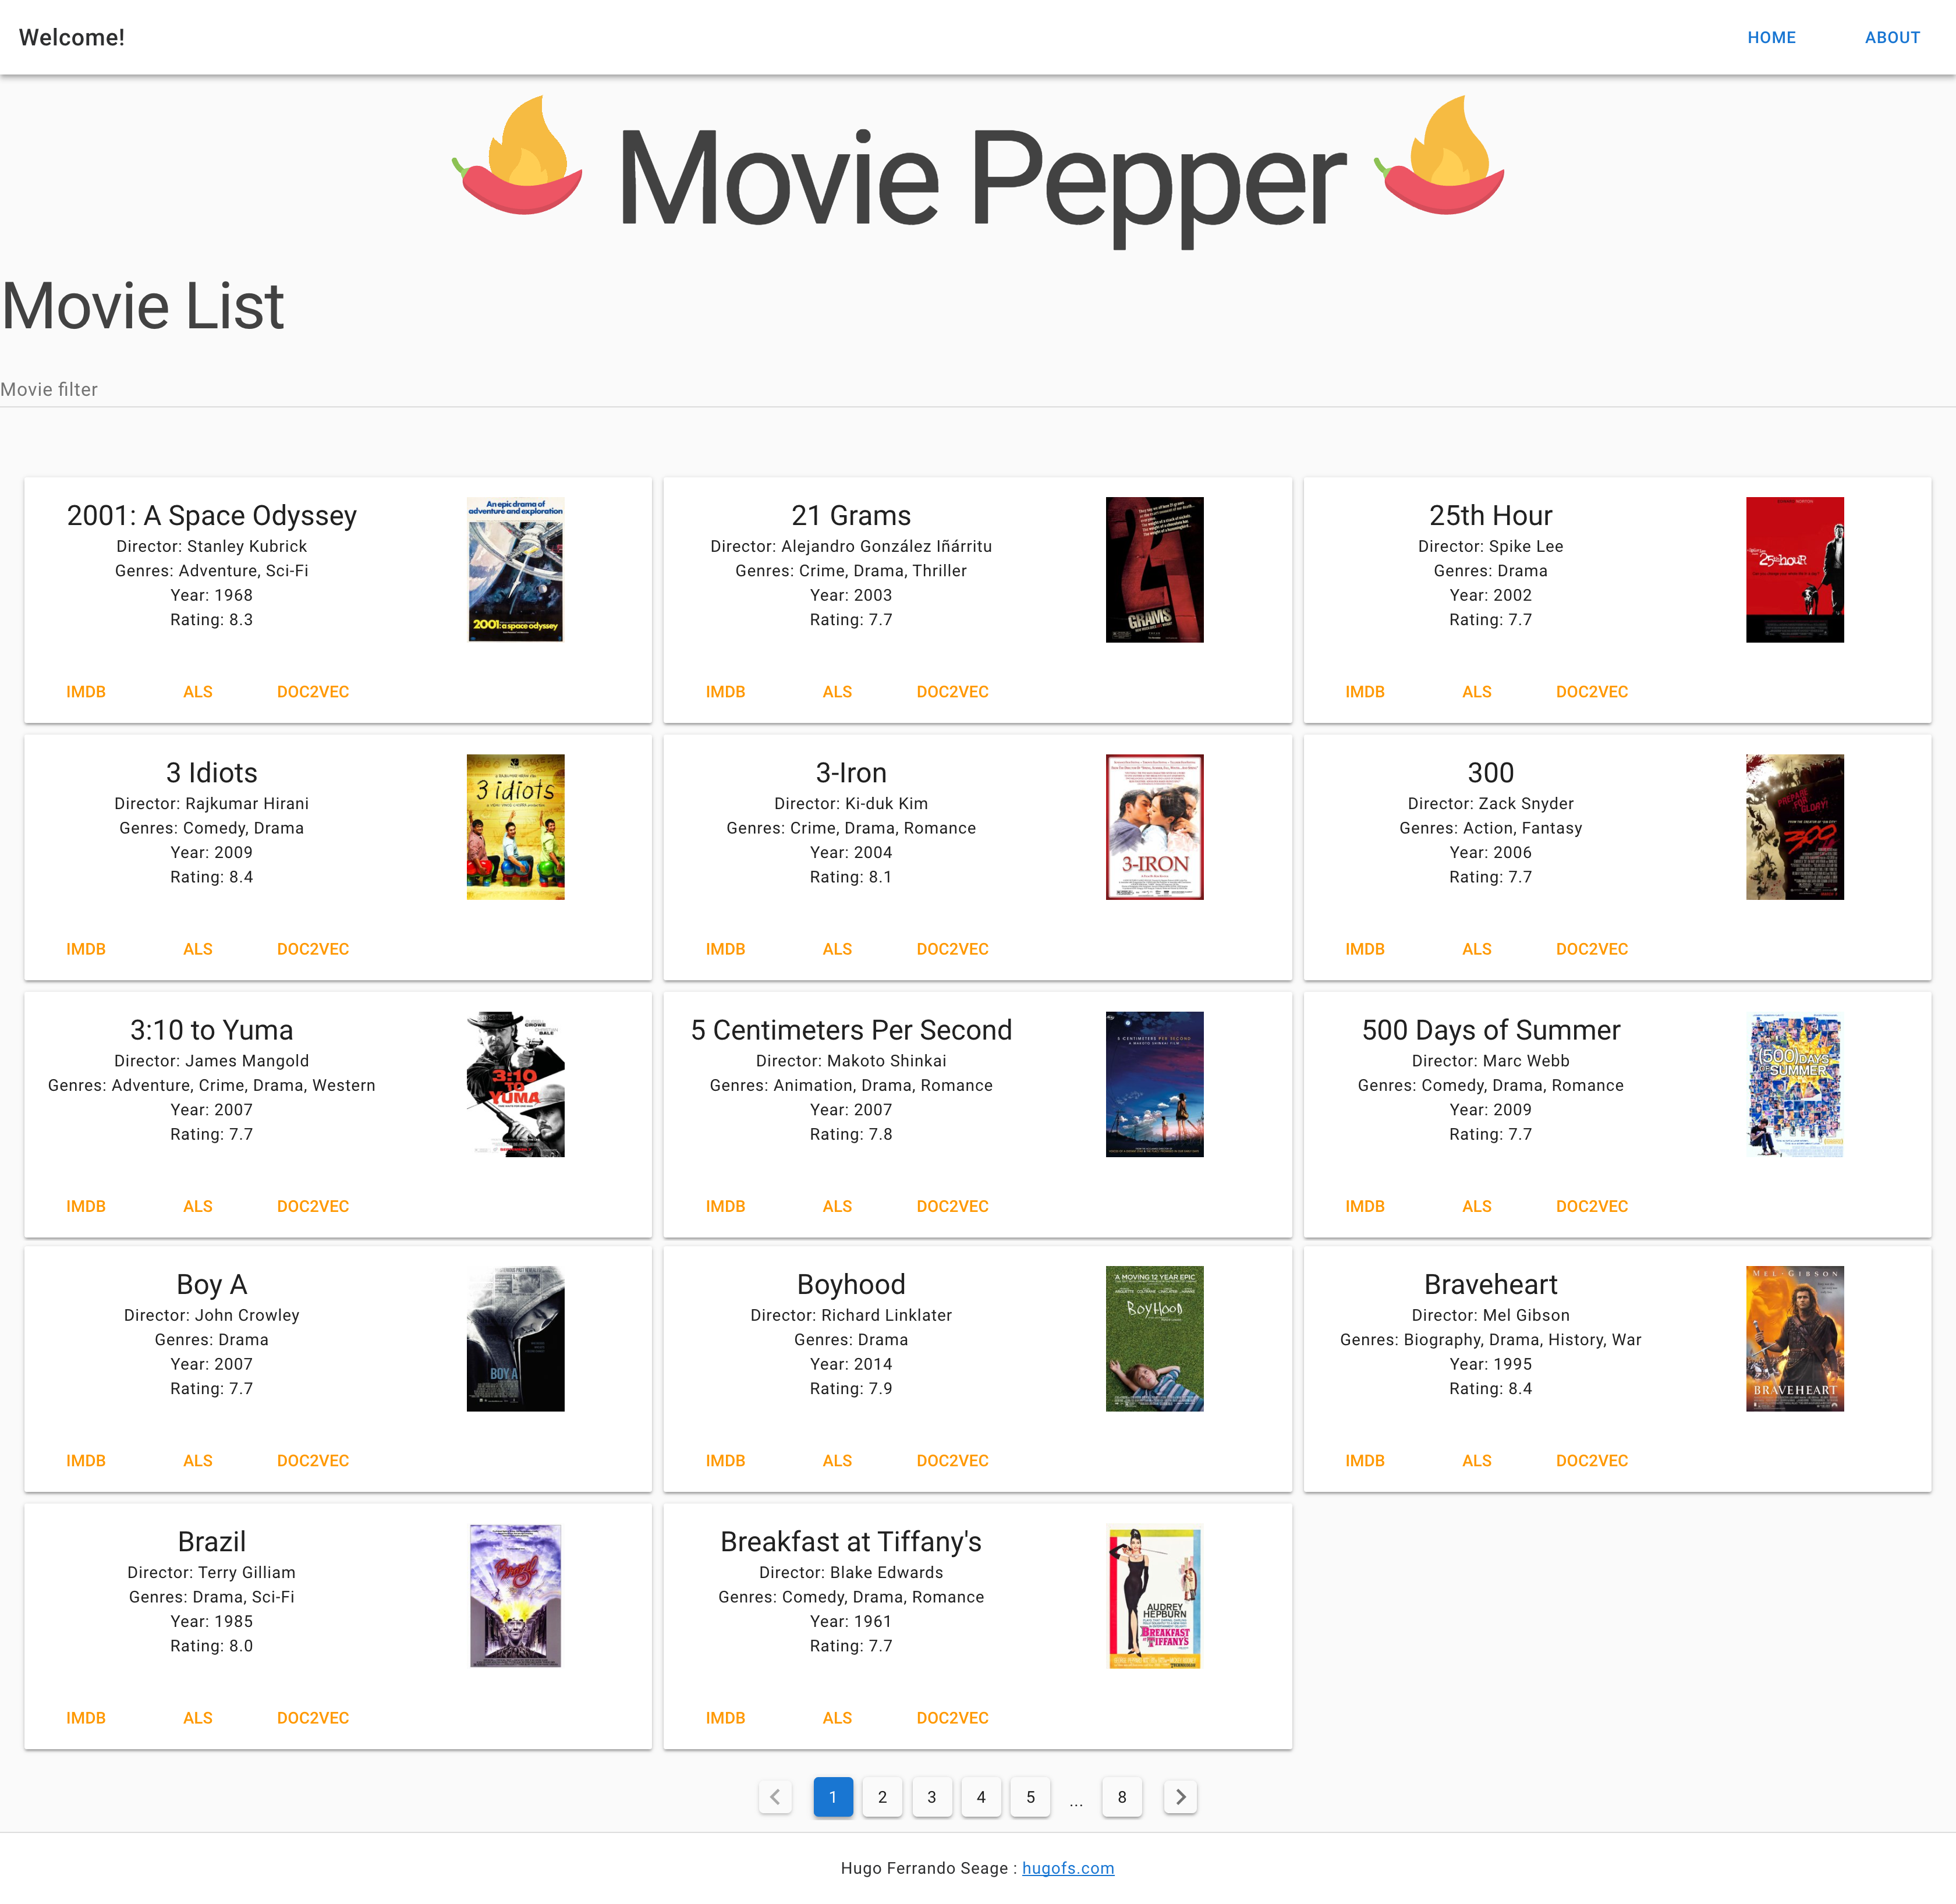
\includegraphics[width=0.7\textwidth]{./figures/int.png}
    \caption{Interfaz de la aplicación}
\end{figure}
\begin{figure}
    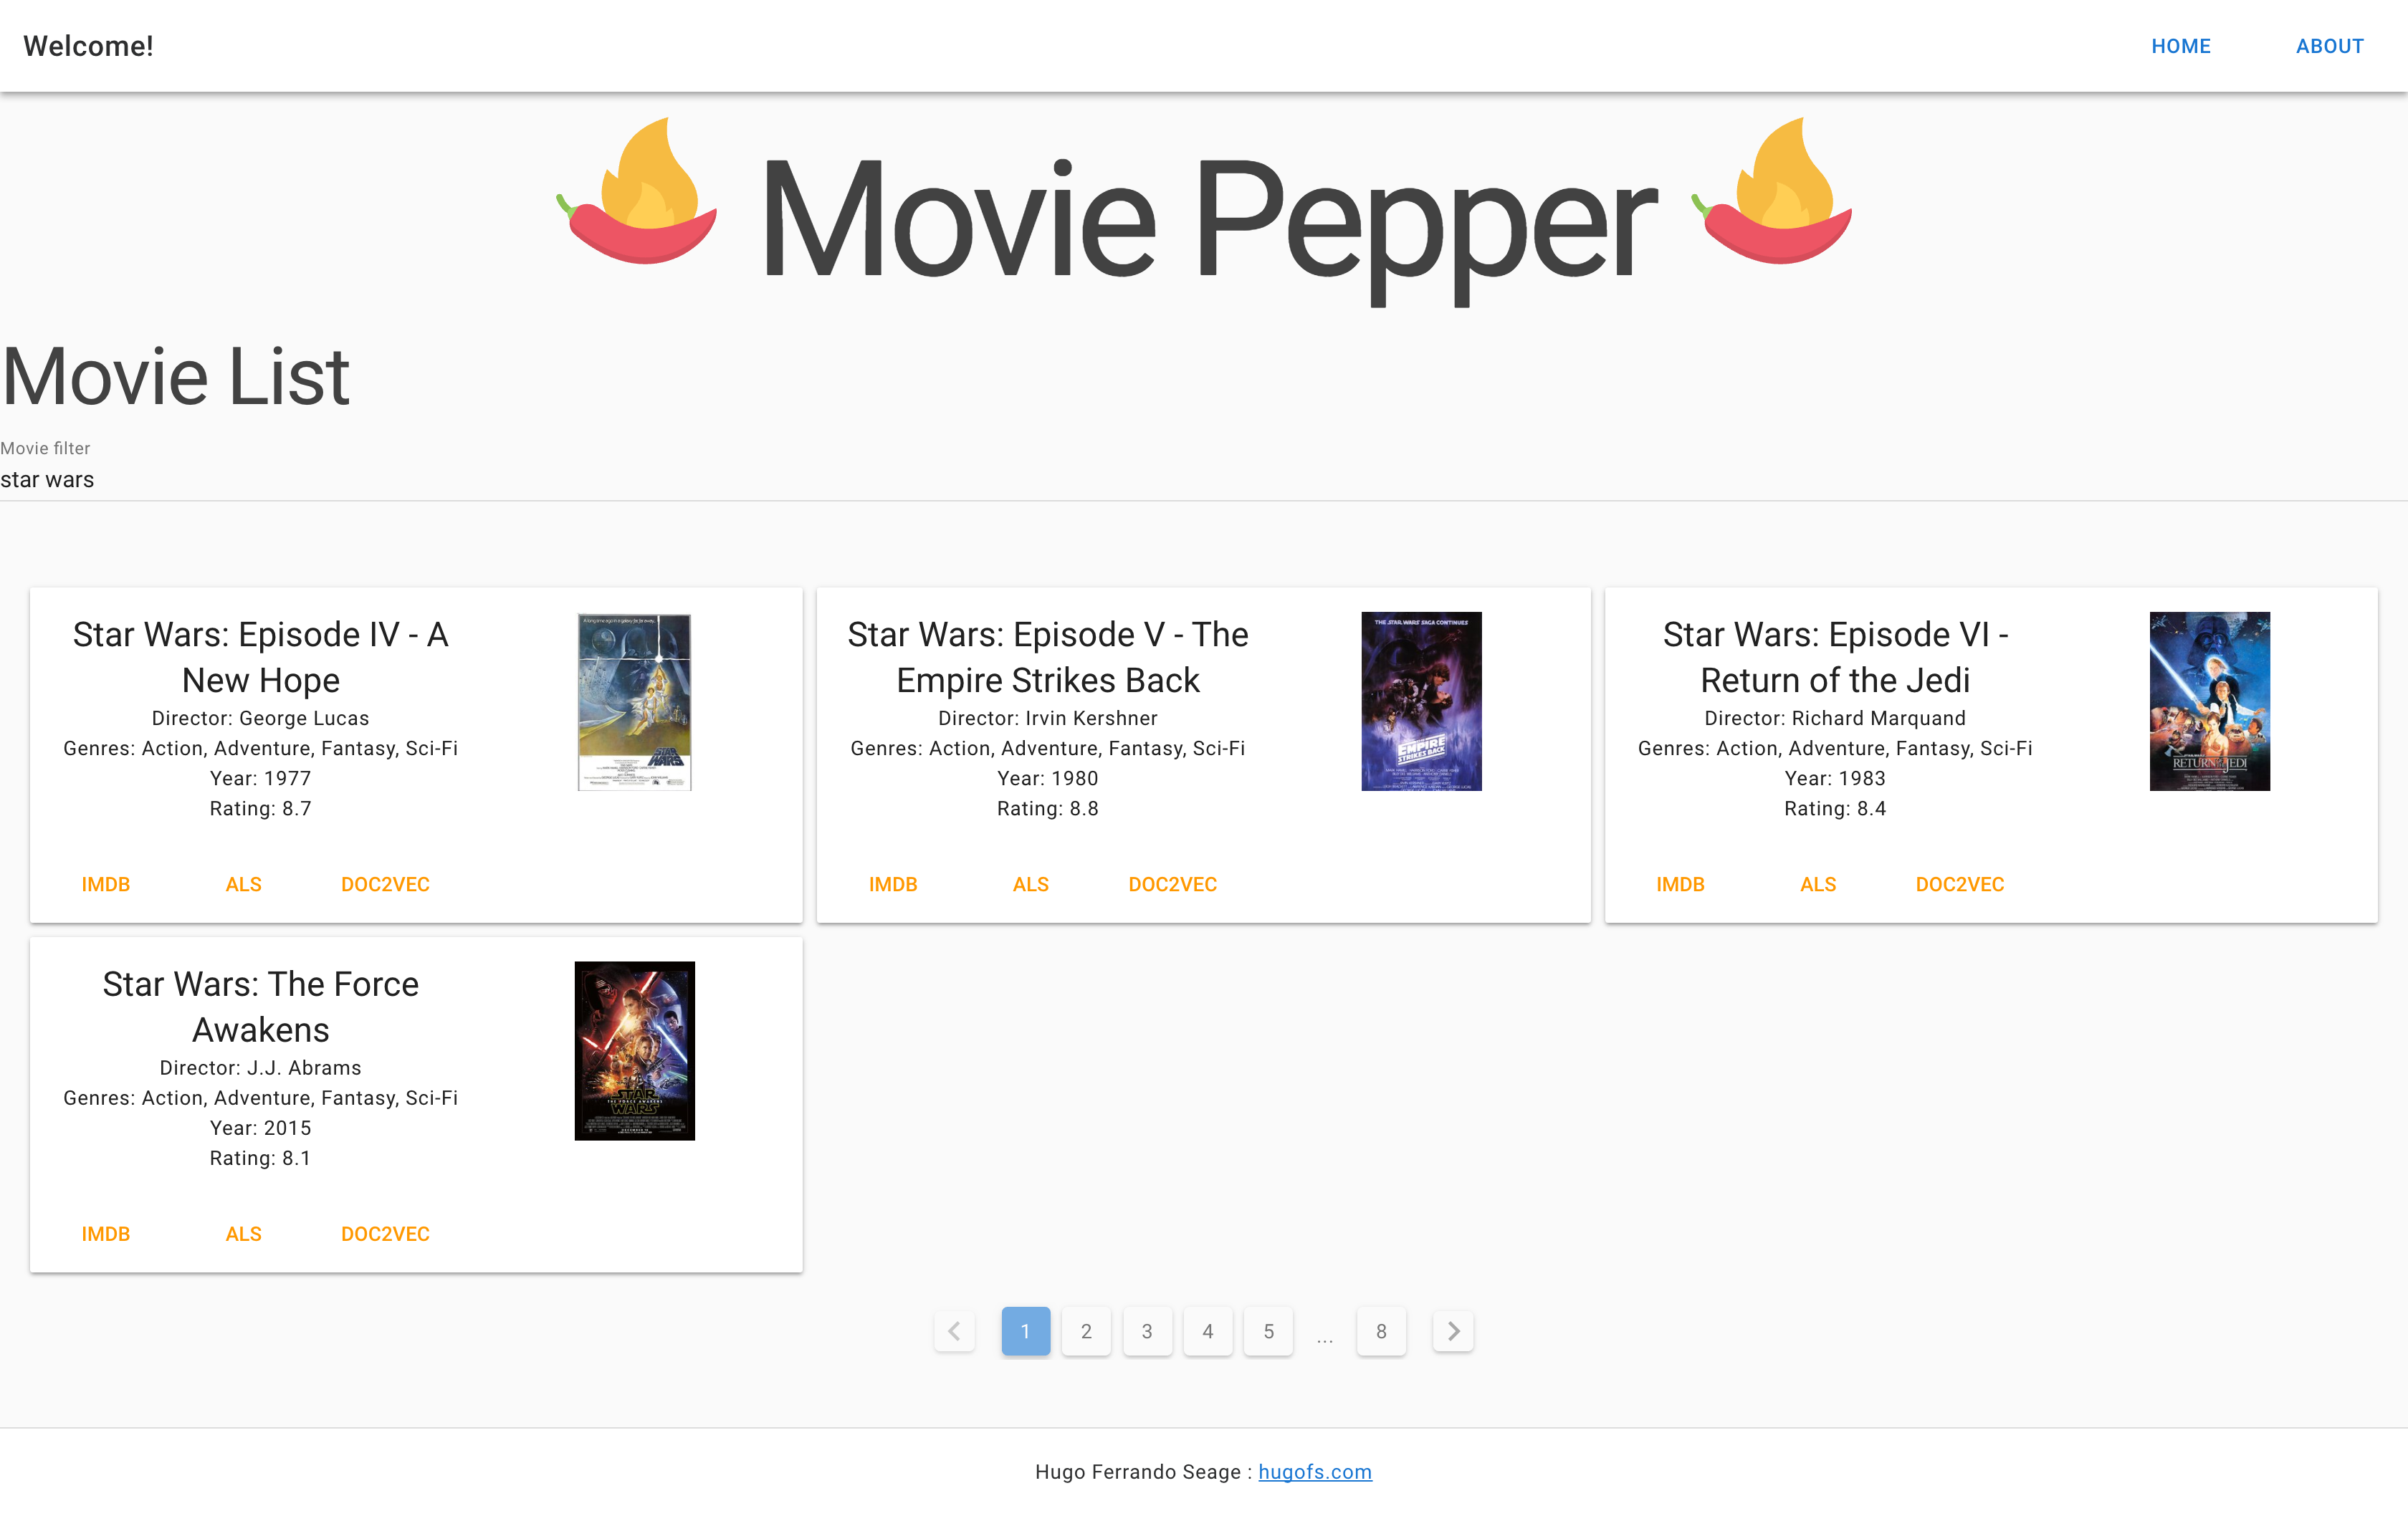
\includegraphics[width=0.7\textwidth]{./figures/int_search.png}
    \caption{Interfaz al buscar}
\end{figure}
\begin{figure}
    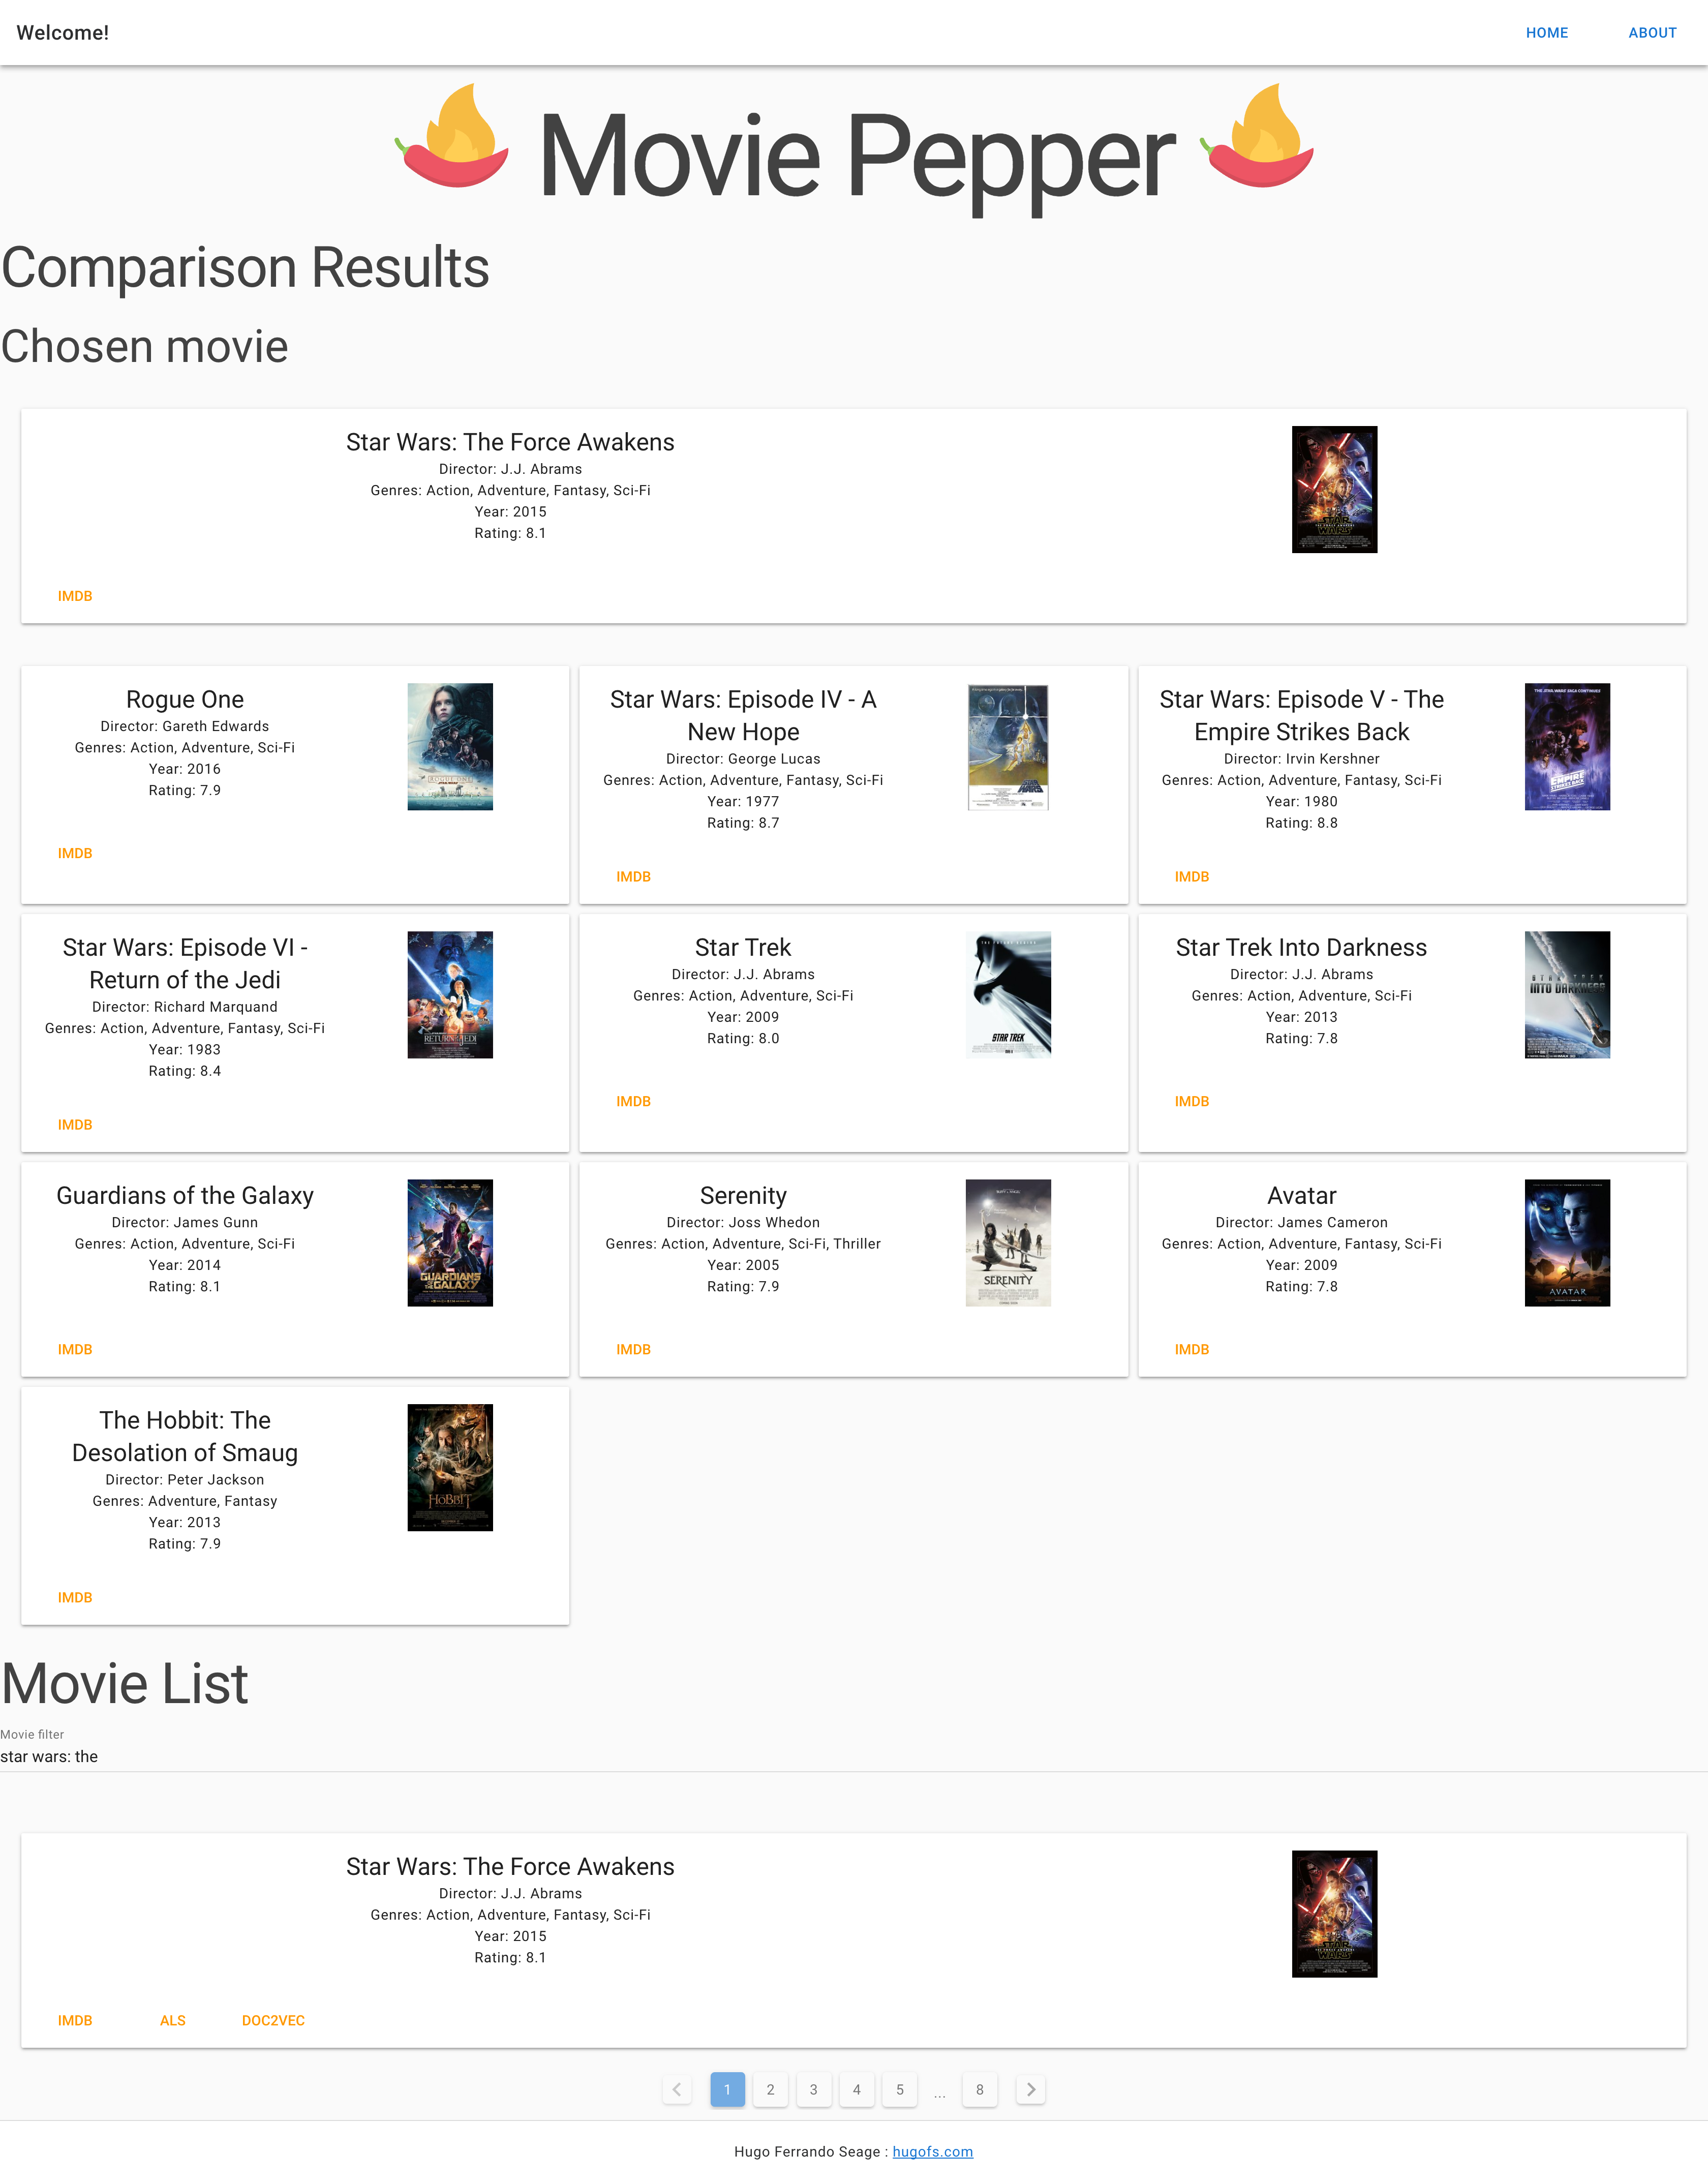
\includegraphics[width=0.7\textwidth]{./figures/int_res.png}
    \caption{Interfaz al mostrar unos resultados}
\end{figure}

\begin{figure}[!htbp]
    \centering
    \begin{tikzpicture}[node distance=2cm]
        \node (moviepepper) [process] {Movie Pepper};
        \node (rest) [process, below of=moviepepper] {REST API};
        \node (movies) [process, right of=moviepepper, xshift=2cm] {/movies};
        \node (lsarec) [process, below of=movies] {/recommend/title};
        \node (d2vrec) [process, below of=lsarec] {/recommend-d2v/title};
        \node (lsamodel) [process, right of=lsarec, xshift=2cm] {\acrshort{lsa}\index{LSA} model};
        \node (d2vmodel) [process, below of=lsamodel] {Doc2Vec model};
        \node (database) [database, right of=movies, xshift=2cm] {Movie store};
        \node (crawl) [process, above of=database] {IMDb crawler};

        \begin{scope}[on background layer]
            \node (bbox) [rectangle,draw,minimum width=2cm] [fit = (movies) (lsarec) (d2vrec),fill=yellow!30,label=above:Endpoints] {};
        \end{scope}

        \draw [arrow] (moviepepper) -- (rest);
        \draw [line] (rest.east) -- (bbox);
        \draw [line] (movies) -- (database);
        \draw [line] (lsarec) -- (lsamodel);
        \draw [line] (d2vrec) -- (d2vmodel);
        \draw [line] (crawl) -- (database);
        \draw [line] (database.east) to [bend left] (lsamodel.east);
        \draw [line] (database.east) to [bend left=50] node[anchor=west] {entrenamiento} (d2vmodel.east);
    \end{tikzpicture}
    \caption{Arquitectura del sistema}\label{arch}
\end{figure}

\chapter{Conclusión}
Completar este proyecto me ha dado una nueva perspectiva en el potencial del procesamiento del lenguaje natural. Modelos como los usados aquí demuestran que es posible para una máquina extraer suficiente información de textos para que se puedan usar en varias aplicaciones.

Estoy más que satisfecho de los resultados que se muestran aquí, pudiendo competir fácilmente con recomendadores usados en servicios comerciales o servicios que llevan operando durante varios años en la industria.

Son herramientas útiles, con un impacto real en los usuarios de los servicios ya que mejora la experiencia y usabilidad. Sin duda, el filtrado colaborativo es una técnica indispensable a la hora de desplegar un servicio de este estilo, pero pienso que estas técnicas son un buen complemento a las recomendaciones personalizadas. Se puede usar para recomendar al terminar de ver contenidos, para nuevos usuarios que aún no han usado la plataforma lo suficiente como para poder hacer recomendaciones personalizadas de manera robusta o incluso son una buena alternativa para usuarios que desean que se respeta su privacidad.

También estoy muy contento del trabajo realizado en el E-Modelo\index{E-Modelo}. Aunque no se haya podido mostrar aquí creo que tiene una potencia enorme, ya que añade toda una nueva dimensión al filtrado colaborativo clásico. Una de las causas de que sus resultados no me hayan convencido como para incluirlo es posiblemente que necesite más una cantidad de datos más grande que los que estaba usando (alrededor de 100.000 textos).

Creo que otro aspecto importante es que el código sea libre para que otras personas puedan probarlo y extenderlo. Por ahora no es posible compartir el código del E-Modelo\index{E-Modelo}, pero es posible que en el futuro sea publicado por el grupo de Big Data Lab de la UEM\@.

\section{Mejoras}
Este proyecto se podría ampliar para incluir otros algoritmos de recomendación basados en distintas técnicas como \acrshort{lda}, cadenas de Markov o clustering. La interfaz podría ser más pulida y ofrecer más información sobre las recomendaciones. Faltan tests unitarios y la habilidad de agregar contenidos fácilmente con el crawler. Las recomendaciones se hacen en tiempo real y no se incluye ningún tipo de cache. Precalcular las recomendaciones o usar algún sistema de cacheado como Service Workers o Redis sería conveniente.

Por supuesto el modelo tiene amplio margen de mejora, ya que algunos resultados son un tanto extraños. También sería una buena opción poder ajustar los parámetros desde la página web. Esto supondría un nivel de complejidad en la arquitectura más alto, ya que el proceso de entrenamiento lleva unos minutos y consume todos los recursos disponibles de la máquina donde se ejecuta. Además habría que guardar cada modelo por separado para evitar recalcular modelos ya entrenados, pero no ocupan poco espacio, y la máquina donde se ejecutan tiene un cantidad muy limitada (20 GB) de espacio de disco.

% Bibliography:
\nocite{*}
\printbibliography{}

\listoffigures
\listoftables

% Index
\printthesisindex{}

\end{document}
